\documentclass[11pt,a4paper]{article}
\usepackage[inline]{enumitem}
\usepackage{amsfonts}
\usepackage{amsmath,amssymb,amsthm}
\usepackage{mathtools}
\usepackage{graphicx,subfigure}
\usepackage[margin=1in,a4paper]{geometry}
\usepackage{algorithm}
\usepackage{algorithmic}
% \usepackage[font= scriptsize]{subcaption}
\usepackage{xcolor}
\usepackage{natbib}
\usepackage{tabu}
\usepackage{multirow} 
\usepackage[colorlinks,citecolor=blue,urlcolor=blue,bookmarks=false,hypertexnames=true]{hyperref} 
%\usepackage[utf8]{inputenc}
\usepackage{newunicodechar}
\providecommand{\keywords}[1]{\noindent\textbf{{Keywords:}} #1}
\usepackage{float}
\usepackage{mathtools}
\usepackage{setspace}
\mathtoolsset{showonlyrefs=true}
\newtheorem{proposition}{Proposition}
\newtheorem{corollary}{Corollary}
\newtheorem{lemma}{Lemma}
\newtheorem{definition}{Definition}
\newtheorem{assumption}{Assumption}
\newtheorem{theorem}{Theorem}
\theoremstyle{remark}
\newtheorem{remark}{Remark}
\newtheorem{example}{Example}
\setlength{\bibsep}{0.0pt}
\allowdisplaybreaks[4]


\graphicspath{{../figures}}


\title{Pricing Financial Derivatives with Operator Network} 

\author{Wenyong Zhang, Chak Wong}

\begin{document}
	
	\maketitle
	
	\begin{abstract}
		Pricing financial derivatives is often done by a computational method under fixed model and contract coefficients. However, understanding the dependence of the derivative price on these coefficients is also important in practice. In this paper, we propose a deep learning method to learn the mapping from the space of time, states, and coefficients to the derivative price. We develop a neural network model in the operator network framework and construct a loss function to train it by solving the backward stochastic differential equation associated with the pricing problem. We test our method in several representative models on both European and path-dependent products. Numerical results demonstrate the ability of our method in learning the complete pricing map.       
	\end{abstract}
	
	\section{Introductions}
	Over the past decades, extensive research results have been developed for pricing financial derivatives. While there exist various analytically tractable cases, numerical methods are generally required for pricing, especially for path-dependent and multi-asset derivatives. A plethora of numerical methods are available, which can be classified into several basic approaches: solving the pricing partial differential equation (PDE) by the finite difference method (\cite{duffy2013finite}) and the finite element method (\cite{hilber2013computational}), Markov chain approximation (\cite{mijatovic2013continuously}, \cite{zhang2019analysis}), Monte Carlo simulation (\cite{glasserman2004monte}), and deep learning.
	
	In recent years, the deep learning approach has become increasingly popular for derivative pricing due to its capability in approximating highly nonlinear functions even in high-dimensional problems. \cite{sirignano2018dgm} develop a deep Galerkin method to solve high-dimensional PDEs arising from option pricing and \cite{gu2021selectnet} introduce a self-paced learning framework to improve convergence. Other papers exploit the connection between nonlinear parabolic PDEs and backward stochastic differential equations (BSDEs) and use deep learning to solve the latter. \cite{han2017deep} and \cite{han2018solving} propose a forward scheme to solve BSDEs by minimizing the error with the terminal condition. 
	\cite{hure2020deep} develop a backward scheme to solve BSDEs by decomposing the global problem into a sequence of smaller learning problems. \cite{beck2021deep} introduce a numerical method that combines operator splitting with deep learning. Various papers price path-dependent derivatives by deep learning; see \cite{jacquier2019deep}, \cite{sabate2020solving}, \cite{feng2021deep}, and \cite{liang2021deep}.
	
	With few exceptions, almost all numerical methods for derivative pricing are developed by assuming coefficients in the model (e.g., interest rate, volatility) and contract (e.g., moneyness) are fixed. In other words, if we want to price the derivative by changing the value of a coefficient, we have to run the numerical method again, which can be time consuming. In practice, pricing a derivative under different coefficient values is required. As an example, sensitivity analysis is often used by derivative traders to understand the impact of changing one coefficient on the derivative price. In addition, a trader may want to know the derivative price in different market scenarios as represented by varying coefficient values. Moreover, financial firms need a derivative price simulator to generate data to learn trading and hedging strategies through reinforcement learning. To achieve computational efficiency in all these applications requires that we obtain the complete mapping from the space of time, states, and coefficients to the derivative price, rather than the partial mapping from the space of time and states to the derivative price with fixed coefficients. 
	
	There is a lack of research in how to obtain the complete pricing map numerically. This problem can be much more challenging than obtaining the partial pricing map with fixed coefficients, as there is significantly more information to learn. Furthermore, some coefficients can be functions instead of real-valued constants, e.g., the risk-free rate and volatility can be time dependent and hence functions of time. This would further complicate the learning problem.
	
	In a recent work, \cite{berner2020numerically} solve parametric Kolmogorov PDEs on a whole space-time region by approximating the PDE solution using a multilevel neural network. They express the PDE solution via the Feynman-Kac formula, which enable them to use supervised learning. However, their network only takes constant coefficients as inputs, and they do not consider coefficient functions. Additionally, they only test their approach on European options under the Black-Scholes model. In another work, \cite{glau2022deep} employ a variant of the highway network to approximate the solution of a family of PDEs for pricing European options under the Black-Scholes model. The neural network is designed to produce the option price as a function of time, state, and model coefficients. Similar to \cite{sirignano2018dgm}, they construct the loss function by directly solving the pricing PDE, where the partial derivatives are computed by automatic differentiation. Like in \cite{berner2020numerically}, only constant coefficients are considered and it is unclear how to deal with coefficients that are functions. The success of their method in pricing European options relies on the decomposition of the option price into an no-arbitrage bound, which is known analytically, and a residual part, which is approximated by the neural network. However, for derivatives with more complex payoffs, this decomposition approach may be inapplicable. 
	
	In this paper, we take an operator perspective to characterize the complete pricing map. Specifically, any coefficient vector gives a pricing function with time and states as its variables. Thus, we have an operator that maps from the coefficient space, which is generally a function space, to the space of pricing functions. The problem then becomes how to learn this operator. Our method is based on the operator network framework, which is proposed in \cite{lu2021learning} based on the universal approximation theorem for nonlinear continuous operators developed in \cite{chen1995universal}. An operator network consists of two critical components: the branch net that models the effect of coefficients and the trunk net that models the effect of time and states. The outputs from these two nets are combined via inner product to yield the final output, which is the derivative price in our problem. We introduce another two components into the operator network framework for derivative pricing. The first one is a neural network called embedding net. As some coefficients are functions, we can end up with a high-dimensional representation of them. The embedding net serves the purpose of dimension reduction by obtaining a lower-dimensional latent representation of these coefficient functions, which is input into the branch net. The second component is a neural network called PI net. The prices of many derivatives are invariant after permuting the assets. The PI net is introduced to capture the property of permutation invariance, which can facilitate convergence for multi-asset derivatives as our experiment shows. 
	
	To train the proposed deep learning model, we consider the BSDE formulation of the derivative pricing problem. BSDEs provide a powerful and unified tool for pricing all kinds of derivatives under general asset price dynamics. We construct a loss function for training that better fits the purpose of our research, and it is different from the loss functions in the literature.
	
	Compared with \cite{berner2020numerically} and \cite{glau2022deep},  our approach is mainly different in two respects. First, we adopt an operator perspective to characterize the complete pricing map, which leads to a network structure that separates the effects of coefficients and $(t,x)$. In comparison, a single network is used in \cite{berner2020numerically} and \cite{glau2022deep} to learn their effects jointly. Second, our adoption of the BSDE formulation is more flexible for dealing with complex path-dependent derivatives, and it can also be extended to incorporate realistic constraints and issues into the pricing problem, such as different borrowing and lending rates and counterparty default risk. 
	
	The rest of the report is organized as follows. Section \ref{sec:OperatorNetwork} introduces the operator network framework for derivative pricing. Section \ref{sec:pricing} presents our design of the pricing operator network and discusses how to construct the loss function by solving the pricing BSDE. Section \ref{sec:numerics} presents numerical results for various derivatives under some standard models. Finally, Section \ref{sec:conclusion} concludes the paper with remarks for future research. 
	
	\section{Operator Network}\label{sec:OperatorNetwork}
    Mapping approximation is a crucial problem in machine learning. Typically, we approximate a function that often maps from a vector space to a real value space. However, there are situations where functions are included as part of the input space. This type of mapping, which incorporates additional functions as inputs, holds significant value, particularly in the context of financial engineering problems such as derivative pricing problem. 
    
    Derivative pricing involves a stochastic model that describes the dynamics of the underlying assets (such as stocks, rates, indices, etc.). The derivative price is typically viewed as a function (pricing function) of time and state of the underlying with a fixed set of coefficients that are related to the model and product (e.g. yield curve, volatility rate, mean reverting rate for models; strike price, barrier level for products, etc.) . To find the relationship between the derivative price and coefficients, this pricing function needs to be extended to a pricing functional which includes the coefficients as an additional variable (This map is called functional since coefficients includes functions). It is important to consider this extended pricing functional for various tasks in the derivative business.  
    
    We formalize this perspective mathematically. Let $u(t,x; a)$ denote a pricing function of time $t$ and state $x \in \mathbb{R}^m$ parametrized by coefficient vector $a = (a_1,\cdots,a_p)$ where each entry of this vector can either be real value (e.g. parameters of the dynamics of underlying assets or product such as mean reverting rate, volatility rate or strike price) or real function (e.g. yield curve or volatility curve). We assume $a\in \mathcal{A}$, which is a space containing functions and real values related to parameters of the pricing function. Therefore, $\mathcal{A}$ is a function space since the components of $a$ can be functions (e.g., the risk-free rate is often described by a curve, which is a function of time ). Then, if we introduce $a$ into the input space of the pricing function, we have the extended pricing functional which is a mapping from  $\mathbb{R}^+ \times \mathbb{R}^m \times \mathcal{A}$ to $\mathbb{R}$ . From another perspective, we can characterize this map by introducing an operator that maps coefficients vector $a$ to pricing functions $u$. Suppose that given $a$, we have a $u(t,x; a)\in \mathcal{U}$, which is a Banach space containing all pricing functions. We consider an operator $\mathcal{G}: \mathcal{A} \rightarrow \mathcal{U}$, which is defined by
    \begin{equation}
    	(\mathcal{G}a)(t, x) := u(t,x; a). \label{eq:operator}
    \end{equation}
    Thus, the problem of pricing the derivative under different coefficients becomes learning the operator $\mathcal{G}$.  Since the component of $a$ consists of functions that are infinite dimensional, we would like to consider how to represent them. Let $\tilde{a} = (\tilde{a}_1,\cdots,\tilde{a}_p)$ be a suitable representation of $a$ (We suppose all entries of $a$ are functions without loss of generality.), which we refer to as function embedding. There are generally two ideas to represent coefficient functions. 
    \begin{itemize}
        \item (\textbf{Basic DeepONet}) The first one is proposed in \cite{lu2021learning} which is using the value of the function $[a(x_1),..., a(x_m)]$ on a specified grid $[x_1,...x_m]$ . However, if variables of this function have a high dimension, this approach would suffer from the curse of dimensionality. 
        \item (\textbf{Add Kernel Operator}) The other idea is expanding the function using a set of basis functions and representing it by the vector of expansion coefficients. For better seeking the expansion coefficients, the more general method is to forward the function into a kernel operator and use some of its outputs as a representation of the input function. The kernel function is denoted as $\psi(x, y) \in C(\mathbb{R}^d \times \mathbb{R}^{\tilde{d}}, \mathbb{R})$ where $\tilde{d} \leq d$ typically. Then for the input function $a(x)$, the kernel operator is defined as:
         \begin{align*}
        	\tilde{a}(y)= \int_{D} \psi(x, y)a(x) dx
        \end{align*}
        Where $D$ is a subset of $ \mathbb{R}^{\tilde{d}}$ and we then choose $[y_1, y_2,...,y_k]$ from the frequency domain and plug into $u(y)$. Then $\tilde{a} = [\tilde{a}(y_1), \tilde{a}(y_2), ..., \tilde{a}(y_k)]$ is the abstract vector which can better represent the function $a(x)$ in a lower dimension.   For choosing of $\psi(x, y)$. We can propose at least two methods:
        \begin{enumerate}
        	\item We can use Fourier transform and output some Fourier modes as the latent representation with the Fourier kernel $\psi(x, y) = e^{-i\pi x^{\top} y}$. This approach is equivalent to projecting the functions onto a set of Fourier basis functions, and selecting only a few dominant Fourier modes can yield a low-dimensional representation of the functions that captures their essential features. This approach can be  computationally more efficient than the grid approach, especially when the input functions have periodic or quasi-periodic behavior. However, selecting appropriate Fourier modes can be challenging and may require some trial and error or domain knowledge. 
        	
        	\item We can use convolution layers to map the original functions to another domain, resulting in a low-dimensional latent representation. We can then concatenate this latent vector with the constant coefficients and input the resulting vector into an FNN to obtain the output of the branch net. This approach can be computationally more efficient than inputting discretized function values directly into the FNN when the number of grid points is large. In this approach, the kernel function is a trainable network or layers (convolution kernel with trainable parameters) which can be represented as: $\psi(x, y) = \psi(x - y; \theta_{\text{CNN}})$. Then $\theta_{\text{CNN}}$ can be involved into trainable variables of the deep operator network.
        	
        \end{enumerate}
        
    \end{itemize}
    
    We introduce the operator network framework proposed by \cite{lu2021learning}. Motivated by the universal approximation theorem for continuous nonlinear operators developed in \cite{chen1995universal} (This will be shown in appendix part), \cite{lu2021learning} approximate $(\mathcal{G}a)(t, x)$ as
    \begin{equation}
    	(\mathcal{G}a)(t, x) \approx G_{\theta}(\tilde{a}, t, x) = \sum_{n=1}^{q} B_n(\tilde{a})\cdot K_n(t, x),\label{eq:G-rep-approx}
    \end{equation}
    where $B_n(\tilde{a})$ and $K_n(t, x)$ are neural networks, and $\theta$ is the vector of parameters in the operator network. This approximation separates the effects of $(t,x)$ and $a$ on the derivative price, so we can build separate models for them.  
    
    In practice, building $2q$ separate neural networks for learning leads to a sophisticated model, which can be difficult to train and is prone to overfitting. We consider the so-called DeepONet, which is proposed in \cite{lu2021learning} and enhanced by \cite{tan2022enhanced}. Figure \ref{fig:deeponet} illustrates its architecture, which consists of two sub-networks named as \emph{branch net} $B(\tilde{a})$ (whose output is in $\mathbb{R}^q$) and \emph{trunk net}  $K(t, x)$ (whose output is in $\mathbb{R}^q$). The branch net outputs the  expansion coefficients for given $\tilde{a}$ while the trunk net outputs values of the basis functions for given $(t,x)$. We then take the inner product of these two output vectors to obtain $G_{\theta}(\tilde{a}, t, x)$. Denote $<\cdot, \cdot>$ as the innerproduct of two vectors, then we approximate $(\mathcal{G}a)(t, x)$ as:
    
    \begin{equation}
    (\mathcal{G}a)(t, x) \approx G_{\theta}(\tilde{a}, t, x) =  <B(\tilde{a}), K(t, x)>,\label{eq:G-rep}
    \end{equation}
    
    For the derivative pricing problem, we further add two components to this framework and will discuss the details of our design in the next section. 
    
    \begin{figure}[htbp!]
    	\centering
    	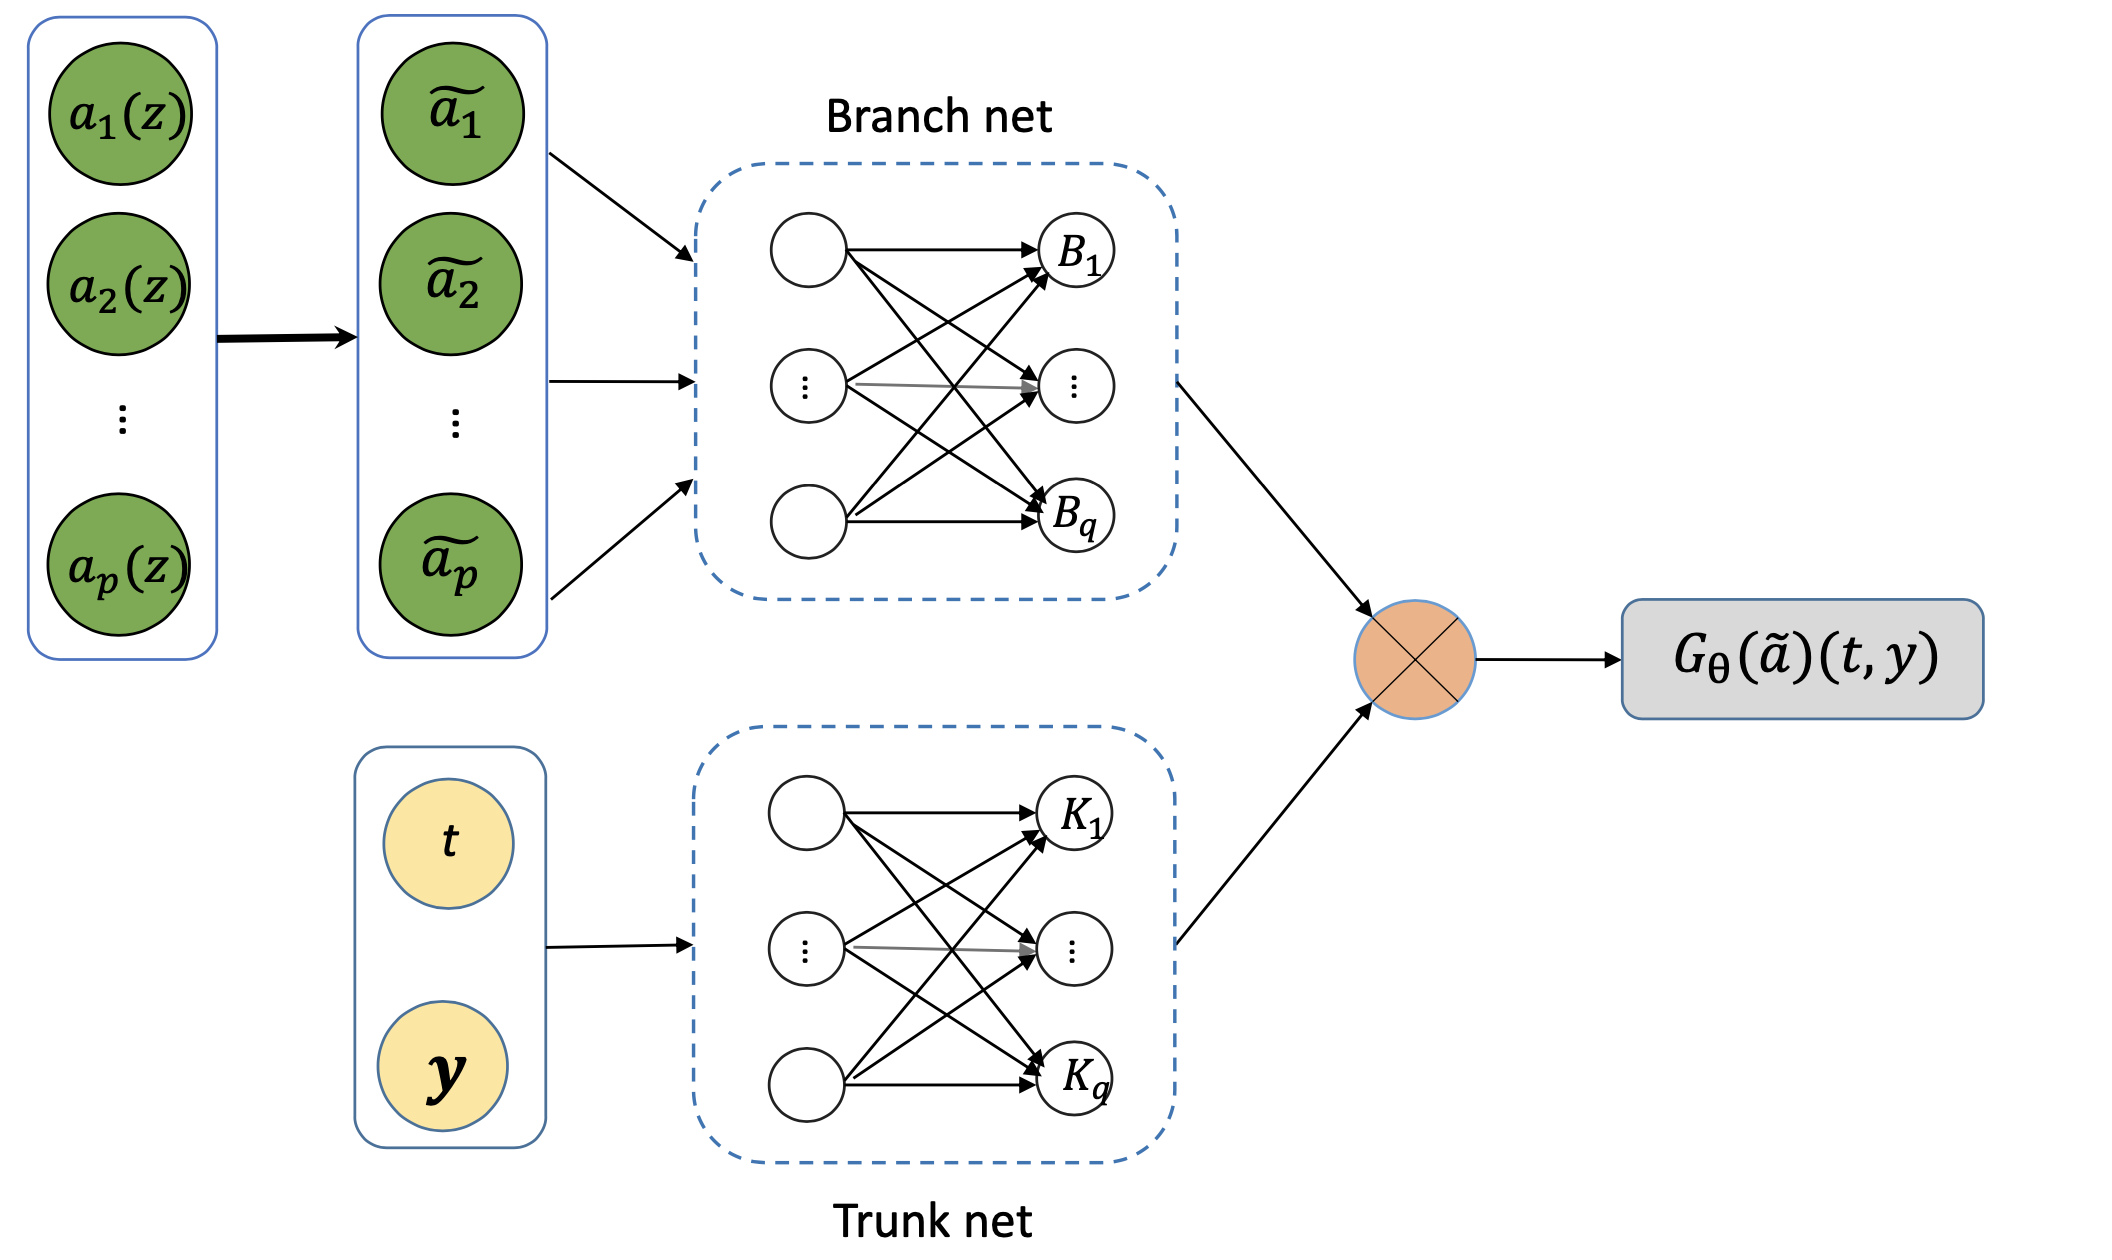
\includegraphics[scale=0.22]{rough_deeponet.png}
    	\caption{Architecture of DeepONet: This figure illustrate the basic structure of the operator network which is composed by branch net and trunk net. For branch net, we do function representation of $a = (a_1,...,a_p)$ by methods provided before (sample on grid or kernel operator) and the send the representation $ (\tilde{a}_1,\cdots,\tilde{a}_p)$ into the branch network and the output a vector of $\mathbb{R}^q$; For trunk net, we can do some processing on $t$ or $y$ (where $y$ in the picture is exactly $x$.) and then input them into a neural network and output a vector of $\mathbb{R}^q$. Finally, we do the innerproduct of outputs from both networks and then obtain the price value given $(t, x; a)$.}
    	\label{fig:deeponet}
    \end{figure}
   

	




	
	\section{Training of Pricing Operator Network}\label{sec:pricing}
	
	We first formulate the derivative pricing problem using BSDEs \footnote{In our problem, we deal with FBSDE, which is Forward-Backward Stochastic Differential Equation. In FBSDEs, we consider two stochastic processes evolving simultaneously: One forward in time and the other backward in time. The forward process (SDE) represents the state of underlying assets and related Markovian variables, while the backward process (BSDE) represents a dual process associated with the pricing function. } , which we will solve by deep learning to obtain the pricing function. We then present our detailed design of the trunk nets in the DeepONet, and develop a loss function for training.  
	
	\subsection{BSDE for Derivative Pricing}
	
	Without loss of generality, we discuss derivative pricing under the time-dependent geometric Brownian motion (GBM) model \footnote{The most general case is the SDE: $\mathrm{d} S_t  = \mu(t, S_t) \mathrm{d} t + \sigma(t, S_t) \mathrm{d} W_t$. Where $a = (\mu, \sigma, \rho, \kappa)$} \footnote{The most general BSDE is $-\mathrm{d} Y_t = -f(t, S_t, Y_t, Z_t) \mathrm{d} t + Z_t dW_t$. Where $f(t,s,y,z)$ is a driver function depends on the product and SDE itself, which is illustrated by Ito formula.}. Our method is applicable to more sophisticated models such as stochastic volatility (SV) and local volatility models. An example considering the Heston's SV model will be presented in experiment section and the example of stochastic local volatilty model (SLV) will be discussed in the extension section. 
	
	On a filtered probability space $(\Omega, \mathcal{F}, \mathbb{P}, \{\mathcal{F}_t, t\ge 0\})$ satisfying the usual hypothesis, consider $d$ underlying assets $S_t = (S^1_t, S^2_t,..., S^d_t)$ with the following dynamics under the risk-neutral measure:
	\begin{align}
		&\mathrm{d} S_t^i  = r(t) S_t^i \mathrm{d} t+\sigma^i(t) S_t^i\mathrm{d} W_t^{i},\quad i=1,\cdots,d, \label{eq:GBM}\\
		& dW^i_tdW^j_t  = \rho_{ij} \mathrm{d}t,
	\end{align}
	where $W_t=(W^1_t,\cdots,W^d_t)$ is a correlated $d$-dimensional Brownian motion with respect to $\{\mathcal{F}_t, t\ge 0\}$, 
	$r(t)$ is the forward rate function, and $\sigma^i(t)$ is the volatility function of asset $i$. We set $\sigma(t)=(\sigma^1(t),\cdots,\sigma^d(t))$, and $\rho=(\rho_{ij})$.
	We assume that $r(t)$ and every $\sigma^i(t)$ are deterministic functions of time. 
	
	The derivative under consideration matures at time $T$ with payoff $G_T$, which can be path dependent. Let $X_t$ be the vector of all related states at time $t$ to determine the derivative price, which may contain more information than the asset prices at $t$. By choosing $X_t$ appropriately, we can write $G_T=g(X_T;a)$ and each product is corresponded to a $g(X_T;a)$. The risk-neutral pricing function is given by
	\begin{equation}
		u(t, x; a) =\mathbb{E}\left[  e^{-\int_t^T r(s) \mathrm{d} s} \left. g(X_T;a) \right| X_t=x\right].\label{eq:price-function}
	\end{equation}
	
	We present three examples of derivative products below. We denote moneyness of an option by $\kappa$, which is defined as the strike divided by the initial asset price (it becomes the average of the initial prices of all assets in the multi-asset case).
	Let $m^i_t=\min_{u\in [0,t]}S^i_u$, which is the running minimum price of asset $i$, and set $m_t=(m^1_t,\cdots,m^d_t)$. We also consider $A^i_t = \exp\left\{\frac{1}{t}\log\left(\int_0^t S^i_s \mathrm{d} s\right)\right\}$, the geometric average price of asset $i$, and set $A_t=(A^1_t,\cdots,A^d_t)$.
	
	\begin{itemize}
		\item European geometric basket call option: $X_t=S_t$, $a=(r(t), \sigma(t), \rho, \kappa)$, and 
		\begin{equation}
			g(X_T;a)=\left(\left(\prod_{i=1}^d S^i_T\right)^{1/d} - \left(\prod_{i=1}^d S^i_0\right)^{1/d}\kappa\right)^+.
		\end{equation}
		
		\item Floating-strike lookback call option: $X_t=(S_t, m_t)$, $a=(r(t),\sigma(t),\rho)$, and 
		\begin{equation}
			g(X_T;a) = \frac{1}{d}\sum_{i=1}^d (S^i_T - m^j_T).
		\end{equation}
		
		\item Geometric Asian call option: $X_t=(S_t, A_t)$, $a=(r(t), \sigma(t), \rho, \kappa)$, and 
		\begin{equation}
			g(X_T;a) = \left(\frac{1}{d}\sum_{i=1}^d A^i_T - \frac{\kappa}{d}\sum_{i=1}^d S^i_0 \right)^+.
		\end{equation}
	\end{itemize}
	
	It is well known that there is a deep connection between derivative prices and solutions to BSDEs. Consider the following BSDE:
	\begin{align}\label{eq:BSDE}
		-\mathrm{d} Y_t &=-r(t) Y_t \mathrm{~d} t- {Z_t}^{\top} \mathrm{~d} W_t, \\
		Y_T &= g(X_T;a),  
	\end{align}
	where $W_t$ is the Brownian motion in \eqref{eq:GBM}. A solution to this BSDE is a pair of processes $(Y_t,Z_t)$ adapted to $\{\mathcal{F}_t,\ t\ge 0\}$. In the solution of the BSDE, $Y_t = u(t, X_t; a)$, which is the derivatives price at time $t$. 
	
	It is important to bear in mind that $X_t, W_t, Y_t,$ and $Z_t$ all depend on the coefficient vector $a$ in our problem. However, to ease notations, we do not explicitly reflect their dependence on $a$ in their notations. 
	
	\begin{remark}
		For path-dependent products, as the previous examples illustrate, additional information must be included in the state vector to determine their prices. While in the examples given, such information can be easily found, more generally one can consider using some representation of the path as a state. See \cite{sabate2020solving}, \cite{jacquier2019deep}, \cite{feng2021deep}, and \cite{bayraktar2022deep} for using path signature and \cite{saporito2020pdgm} for using LSTM to solve the pricing problem in various settings.
	\end{remark}
	
	
	
	
	\subsection{Trunk Network Design-Adding Permutation Invariant Layers}
	We discuss further design of the  trunk net.  For single asset option pricing, it is sufficient to input the time and state variables into an FNN, as shown in \cite{lu2021learning}. However, for multi-dimensional tasks, inputting high-dimensional states directly into the FNN leads to a significant increase in the number of parameters to train, which can cause various convergence issues. Fortunately, payoffs of multi-asset options often have a symmetric structure, meaning that the asset price variables of their pricing functions are exchangeable. Below are three common European-style multi-dimensional payoff functions (Where $I$ is the strike price which is predetermined):
	\begin{equation}
		g(X_T; a)= \begin{cases}\left(\max \left(S^1_T, \ldots, S^d_T\right)-I\right)_{+}, & \text {(basket call on max), } \\ \left(\frac{1}{d}\sum_{i=1}^d S^i_T-I\right)_{+}, & \text {(basket call on sum), } \\ \sum_{i=1}^d 1_{\{S^i_T \geq I\}}, & \text {(basket sum of binary options).}\end{cases}
	\end{equation}
	In the above payoff functions, if we permute the underlying assets, the option's payoff and price remain unchanged. We call this property permutation invariant (PI). 
	
	\cite{germain2022deepsets} proposed a symmetric neural network to parameterize PI functions, which we employ in our problem. We call it as \emph{PI net} and explain its structure. Let $x_i$ denote the state variable vector of asset $i$ with length $n_x$, and we set $x = (x_1,...,x_d)$. For each $x_i$, we input it into an FNN $\varphi$, which is shared among all the assets. This network maps $x_i\in\mathbb{R}^{n_x}$ to $\varphi(x_i)\in\mathbb{R}^k$. Set $\varphi(x)=(\varphi(x_1),\cdots,\varphi(x_d))$, which is a latent representation of $x$. We output from the PI net
	\begin{equation}
		\Phi(x)= \mathfrak{s}\left(\varphi\left(x\right)\right),
	\end{equation}
	where $\mathfrak{s}$ is a symmetric function in its variables. Below are some examples of symmetric functions and all of them operate component-wise. 
	\begin{itemize}
		\item Max-pooling: $\mathfrak{s}(x)=\max \left(x_1,...,x_d\right)$.
		\item Sum: $\mathfrak{s}(x)=\sum_{i=1}^d x_i$.
		\item Average: $ \mathfrak{s}(x)=\frac{1}{d}\sum_{i=1}^d x_i$.
	\end{itemize}
	The choice of the symmetric function is clearly determined by the product's payoff. For example,  we use the max-pooling function for the basket call on max, and the sum function for the basket call on sum. The architecture of the PI net is illustrated in Figure \ref{fig:sym}.
	  	\begin{figure}[h!]
	  	\centering
	  	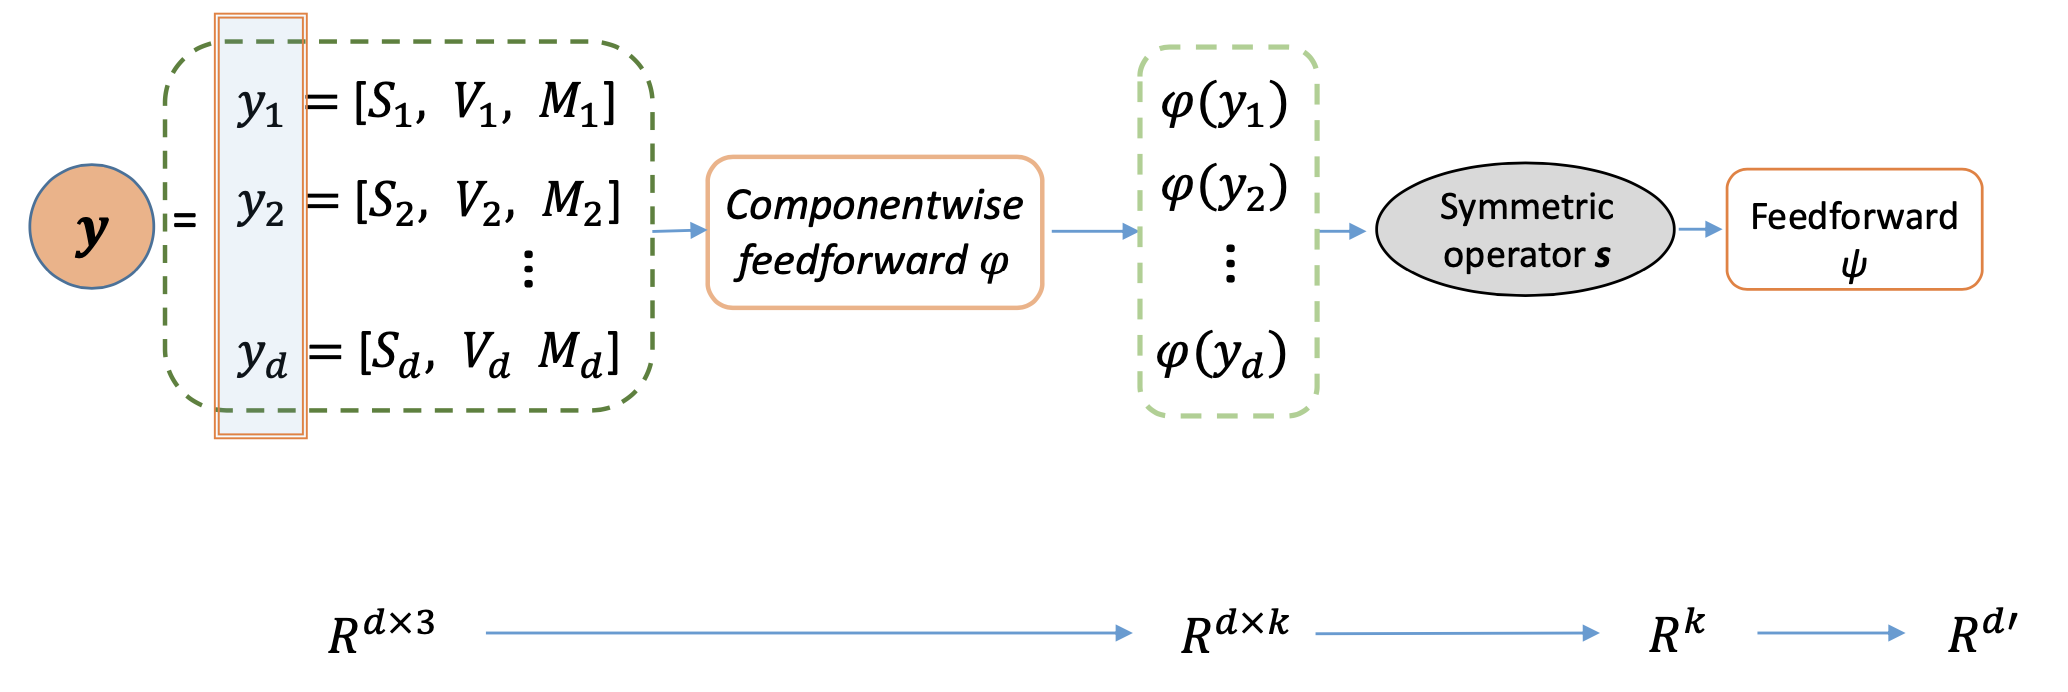
\includegraphics[scale=0.20]{pi_net.png}
	  	\caption{Architecture of the PI net: First we seperate the state of each assets and the forward the state of each asset into a neural network $\varphi(\cdot)$ seprately and the we get a matrix in $\mathbb{R}^{dxk}$. Then we pass this matrix into the symmetric operator (e.g. we calculate the average on the dimension of $d$). Finally we forward the output into a ordinary FNN and we have the output which is invariant of the permutation of underlying assets.}
	  	\label{fig:sym}
	  \end{figure}
	After the propagation of the PI net, we combine its output $\Phi(x)$ with the time variable $t$ and feed them into the trunk net, whose architecture is shown in Figure \ref{fig:detailed_deeponet}. As the output of the PI net is invariant by permutation, the output of the trunk net also has this property. This allows the operator network to capture the PI property of the derivative price. 
	
	We call the operator network designed for our problem pricing operator network (PONet).
	
	\begin{figure}[htbp!]
		\centering
		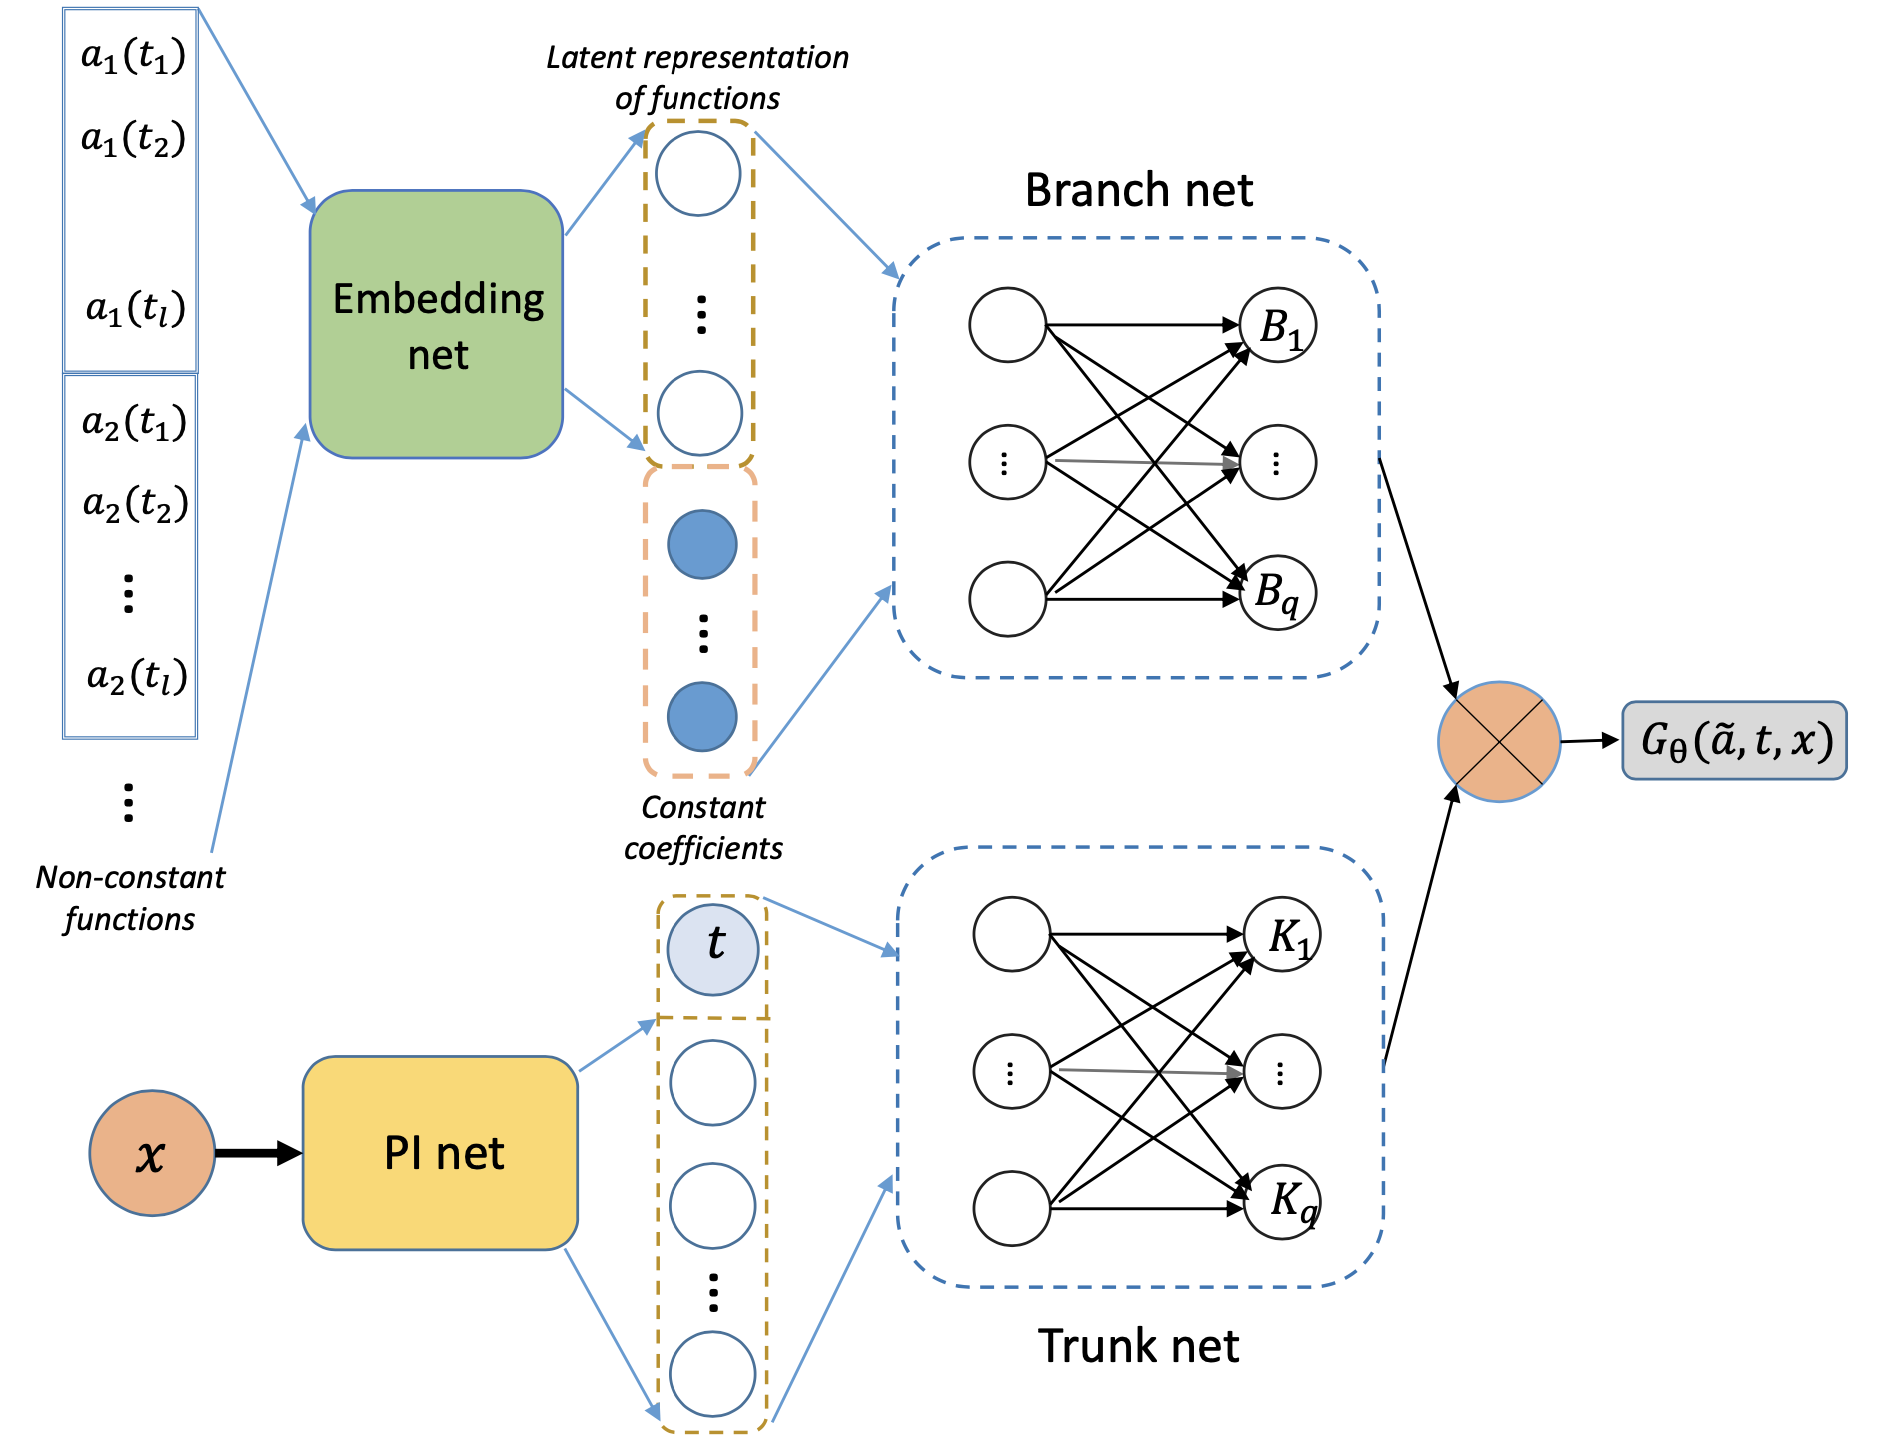
\includegraphics[scale=0.22]{detailed_deeponet2.png}
		\caption{Architecture of the pricing operator network (PONet): This is the detailed forward propagation of out network. For branch network: we first forward the functions into a embedding net which plays a role on function representation and it can be parametrized and unparameterized based on the kernel operator we have chosen then we concatencate the representation and real valued coefficients to a unified tensor and send it into the branch network; For trunk network: we first forward state variables into the permutation invariant network and concatencate the output with the time variable and finally send them into the trunk network.}
		\label{fig:detailed_deeponet}
	\end{figure}
	
	\subsection{Loss Function}
	
	In the literature, the BSDE \eqref{eq:BSDE} is solved for fixed $a$ . We discuss the loss function under SDE with and without jump diffusion (We discuss loss function without jump in this section, things with jump is leaved in the extension section.). For simplicity, for non-jump case, we use time-dependent GBM as the example to discuss the loss. We also need to obtain the dependence of the BSDE's solution on $a$. The entire mapping from $(a,t,x)$ to the derivative price is approximated by the PONet $G_{\theta}(\tilde{a},t,x)$. To learn the optimal $\theta$, we need a loss function for training. 
	
	Given $a$, we construct a loss function $\mathcal{L}(\theta;a)$ based on the discretized BSDE. Then we take expectation over a distribution $\mu$ from which we sample the coefficient vector $a$. This yields the following loss function for the PONet:
	\begin{equation}
		\mathcal{J}(\theta)=\mathbb{E}_{a \sim \mu}\left[\mathcal{L}(\theta;a)\right].
	\end{equation}   
	
	\subsubsection{Loss Function under Diffusion Processes}
	In this report, we discuss the construction of the loss function in the context of diffusion processes (non-jump processes). To simplify the explanation, we utilize a time-dependent Geometric Brownian Motion (GBM) process as an example (Other underlying assets follow the same routine of loss function construction.). This choice allows us to better illustrate the formulation of the loss function. However, it's important to note that for processes involving jump diffusion, the corresponding Backward Stochastic Differential Equation (BSDE) and loss function differ slightly but pose a greater challenge. Therefore, we will address pricing under jump processes in the extension section.
	We next explain how to construct $\mathcal{L}(\theta;a)$ for given $a$ under GBM model. Recall the BSDE in intergal form:
	\begin{equation}
		Y_t = g(X_T; a) - \int_t^T r(s) Y_s \mathrm{~d} s  - \int_t^{\top} {Z_s}^{\top} \mathrm{~d} W_s,\quad t\in[t_0,T].
	\end{equation}
	We consider a time grid: $0 = t_0 < t_1 < ... < t_{N}=T$ which is indexed by $\left\{0, 1, \cdots, N\right\}$. For simplicity, we assume the time points are equally spaced with time step $\Delta t$. Let $\Delta W_{t_n}:=W_{t_{n+1}}-W_{t_n}$. We discretize the SDE \eqref{eq:GBM} using the Euler scheme as
	\begin{equation}
		S_{t_{n+1}}^i \approx S_{t_n}^i + r(t_n) S_{t_n}^i \Delta t + \sigma^i(t_n) S_{t_n}^i\Delta W_{t_n},\quad i=1,\cdots,d, \label{eq:GBM-dist}
	\end{equation}
	For the BSDE, we discretize it as 
	\begin{align}\label{eq:dist-BSDE}
		Y_{t_N} & = g(X_{t_N}; a),  \\
		Y_{t_n} &\approx Y_{t_{n+1}} - r(t_{n+1}) Y_{t_{n+1}}\Delta t  -  Z_{t_n}^\top \Delta W_{t_n},\ \ n=N-1,\cdots,0. 
	\end{align}
	The output from the PONet, $G_\theta(\tilde{a},t_n,x)$ approximates $Y_{t_n}$ given $X_{t_n}=x$.  Then we construct the loss function. The loss function is seperated into two parts. The one is interior loss, which is to minimize the square error of the residual part of the BSDE \ref{eq:BSDE} (The first line of the equation); the other is the terminal loss, which is to minize the distance between the value yield from the network and the exact terminal payoff (The second line of the equation). Then we sum them up to form the loss given $a$. We give the formulation of these two loss functions:
	\begin{itemize}
		\item  The interior loss which is to optimize the interior condition is:
		 \begin{align}
		 	\mathcal{L}_{\text{interior}}(\theta; a) =\frac{1}{M}\sum_{m=1}^M \sum_{n=0}^{N}\left(g(X^m_{t_N}; a) - G_{\theta}(\tilde{a}, t_n, X^m_{t_n}) - \sum_{k=n}^{N-1}r(t)G_{\theta}(\tilde{a}, t_k, X^m_{t_k}) \Delta t + (Z^m_{t_k})^{\top}\Delta W^m_{t_k}\right)^2
		\end{align}
		which means that we need to enforce the approximated value match all the ground truth value at each time step stemed from the terminal payoff through the BSDE \ref{eq:BSDE}. In this function, $X_{t_n}^{i,m}$ denotes the state vector at time $t_n$ of asset $i$ on path $m$ (In GBM case, $X^m_{t_n} = S^m_{t_n} $; in stochastic volatility case, $X^m_{t_n} = (S^m_{t_n}, V^m_{t_n})$; In Asian option case, $X^m_{t_n} = (S^m_{t_n}, A^m_{t_n})$ etc.) and $\Delta W^m_{t_k}$ denotes the Brownian increment in the time interval $[t_k, t_{k+1}]$ of the $m$-th path. The control term $Z^m_{t_n}$ for $n=0,...,N-1$ and $m=1,...,M$ is given as:
		\begin{equation}\label{eq:Z}
			Z_{t_n}^m = \sigma(t)\circ S_{t_{n}}\circ\nabla_X G_{\theta}(a, t_{n}, X_{t_n}^{m}),	
		\end{equation}
		\item The terminal loss function is given as:
		\begin{align}
				\mathcal{L}_{\text{terminal}}(\theta; a)  = \frac{1}{M}\sum_{m=1}^M\left(G_{\theta}(\tilde{a}, t_{N}, X_{t_N}^m) - g(X_{t_N}^m; a)\right)^2.	
		\end{align}
		This loss enforce the value given at the terminal date match the exact terminal payoff $g(X^m_{t_n}, a)$.
	\end{itemize}
	Then the loss function $\mathcal{L}(\theta;a)$ is given by:
	\begin{equation}\label{eq:loss-a}
		\mathcal{L}(\theta;a) =  \mathcal{L}_{\text{interior}}(\theta; a) + 	\mathcal{L}_{\text{terminal}}(\theta; a) 
	\end{equation}
	
	\iffalse
	\begin{itemize}
		\item Step 1: For $m=1,\cdots, M$, generate a path of the price process for each asset using \eqref{eq:GBM-dist}. On each path, calculate the related states at each time point. We denote the state vector at time $t_n$ of asset $i$ on path $m$ by $X_{t_n}^{i,m}$ and $X_{t_n}^{m}$ is the collection of all $X_{t_n}^{i,m}$. We also keep the generated Brownian increment path $\{\Delta W_{t_n}^m: n=0,\cdots, N-1\}$.
		
		\item Step 2: For $n=0,...,N-1$ and $m=1,...,M$, calculate 
		\begin{equation}\label{eq:Z1}
			Z_{t_n}^m = \sigma(t)\circ S_{t_{n}}\circ\nabla_X G_{\theta}(a, t_{n}, X_{t_n}^{m}),	
		\end{equation}
		where $\circ$ denotes Hadamard product. The gradient calculation is accomplished by automatic differentiation of a neural network with respect to its input. 
		
		\item Step 3: Set $Y_{t_N}^m = g(X_{t_N}^m; a)$ for $m = 1, 2,...,M$. At $t_{N}$, set 
		\begin{equation}
			L = \frac{1}{M}\sum_{m=1}^M\left(G_{\theta}(\tilde{a}, t_{N}, X_{t_N}^m) - g(X_{t_N}^m; a)\right)^2.	
		\end{equation}
		
		
		\item Step 4: For $n= N-1, ..., 0$, we calculate
		\begin{equation}
			Y_{t_n}^m  = Y_{t_{n+1}}^m - r(t_{n+1})Y_{t_{n+1}}^m \Delta t - (Z^{m}_{t_n})^{\top}\Delta W_{t_n}^m,\quad m = 1, 2,...,M. \label{eq:Y-recursion}
		\end{equation}
		We update $L$ as 
		\begin{equation}
			L = L + \frac{1}{M}\sum_{m=1}^M\left(G_{\theta}(\tilde{a}, t_{n}, X_{t_n}^m) - Y_{t_n}^m \right)^2.
		\end{equation}
	\end{itemize}
	The loss function $\mathcal{L}(\theta;a)$ is given by the output from step 4, i.e., 
	\begin{equation}\label{eq:loss-a}
		\mathcal{L}(\theta;a)=\frac{1}{M}\sum_{m=1}^M\sum_{n=0}^N\left(G_{\theta}(\tilde{a}, t_{n}, X_{t_n}^m) - Y_{t_n}^m \right)^2.
	\end{equation}
	\fi
	
	\noindent To obtain $\mathcal{J}(\theta)$, we need to sample $a$ from distribution $\mu$. Suppose that we have a batch of sampled coefficients $\left\{a_1,\cdots,a_B\right\}$. We calculate $\mathcal{J}\left(\theta\right)$ by 
	\begin{equation}\label{eq:total-loss}
		\mathcal{J}\left(\theta\right) = \frac{1}{B}\sum_{j=1}^B \mathcal{L}(\theta; a_j).
	\end{equation}
	To learn $\theta$, we minimize $\mathcal{J}\left(\theta\right)$ by stochastic gradient descent. In each iteration, a batch of $B$ coefficients are sampled and for each sampled coefficient vector $a_j$, $M$ price paths are generated to calculate $\mathcal{L}(\theta; a_j)$. A summary of the training algorithm is presented in  \ref{sec:euro}.
	
	\noindent \textbf{Testing Design}: One method to test the loss function is to plug the analytical solution into the loss function to check whether the loss function value is close to zero. For BSDE under GBM, we use the Black-Scholes formula as the operator network and calculate the loss function on this model.
	
	
	
	\subsubsection{Algorithm of European Style Products} \label{sec:euro}
	We summarize the training framework of European style problem on a certain time interval $[T_1, T_2]$. In this framework, the initial time $t_0$ is corresponded to $T_1$ and terminal time $T$ is corresponded to $T_2$. The algorithm is states as \ref{alg:euro_algo}:	
	\begin{algorithm} [htbp!]
		%\caption{Training of the PONet}
		\begin{algorithmic}[htbp!] 
			\caption{Training of the Pricing Operator Network on $[T_1, T_2]$}\label{alg:euro_algo}
			\STATE Specify the sampling distribution $\mu$ and initialize $\theta$.
			\FOR{$i= 1, 2,...$}{ 
				\STATE Sample a batch of coefficients  $\left\{a_j,\ j=1,\cdots, B\right\}$ from $\mu$.
				\STATE For each $j$, generate $M$ asset price paths on $[T_1, T_2]$ under $a_j$ and calculate $\mathcal{L}(\theta; a_j)$. .
				\STATE Calculate $\mathcal{J}(\theta)$. 
				\STATE Update $\theta$ by gradient descent. 
			}
			\ENDFOR
			\RETURN  The well trained operator network $u_{\theta}(t, x; a)$ defined on $[T_1, T_2]$.
		\end{algorithmic}
	\end{algorithm}
	
	\noindent For a specific product, we need to clarify several issues:
	\begin{itemize}
		\item The coefficients $a$ from underlying SDE (e.g. rate curve, volatility curve, correlation coefficients, etc.) and  product (e.g. barrier level, strike price, etc.); 
		\item The terminal payoff $g(X_{\tau_N}; a)$ which can be path dependent; 
		\item The Markovian variables for path-dependent product.
	\end{itemize}
	
	\subsection{Framework with Early Exercise Features}
	The most common type of early exercise derivatives is Bermudan options, one can exercise the product at a series of early exercise times. Denote $\mathcal{T}:=\left\{\tau_0=0, \tau_1, \ldots, \tau_k,\cdots,\tau_N=T\right\}$. be a collection
	of pre-determined time stamps on $[0, T]$. For Bermudan type options, the buyer has the right to exercise
	the option and obtain payoff $g(\tau, X_{\tau}; a), \tau \in \mathcal{T}$. Consequently, the fair price at time $t$ can be written as:
	\begin{equation*}
		u(t, x; a)=\sup _{\tau \in \mathcal{T}, \tau \geq t} \mathbb{E}\left[e^{-\int_{\tau}^T r(s) ds} g\left(\tau, X_\tau; a\right) \mid X_t = x\right]
	\end{equation*}
	Fortunately, from the method in \cite{gao2022convergence} and \cite{wang2018deep}, we have the formulation of the BSDE of Bermudan derivatives. We express the BSDE with integral form::
	\begin{equation} \label{bsde: amc}
		\left\{\begin{array}{l}
			Y_T=g\left(T, X_T; a\right) \\
			Y_t=Y_{\tau_{k+1}}-\int_t^{\tau_{k+1}} r(s)Y_s \mathrm{d} s-\int_t^{\tau_{k+1}} {Z_s}^{T} \mathrm{~d} W_s, \quad t \in\left(\tau_k, \tau_{k+1}\right), k=N-1, \ldots, 0, \\
			Y_{\tau_k}=\max \left(g\left(\tau_k, X_{\tau_k}; a\right), Y_{\tau_{k+1}}-\int_{\tau_k}^{\tau_{k+1}} r(s)Y^a_s \mathrm{d} s-\int_{\tau_k}^{\tau_{k+1}} {Z_s}^{T} \mathrm{~d} W_s\right) .
		\end{array}\right.
	\end{equation}
	Then this kind of problem can be decomposed into several sub-problem while each problem is corresponded to an European pricing problem.. Then the problem can be solved by a recursive procedure:
	\begin{itemize}
		\item When $t \in(\tau_{N-1}, \tau_{N}]$, solve the BSDE problem:
		\begin{align*} 
			Y_{\tau_N}&=g\left(\tau_N, X_{\tau_N}; a\right) \\
			Y_t &=Y_{\tau_{N}}-\int_t^{\tau_{N}} r(s)Y_s \mathrm{d} s-\int_t^{\tau_{N}} {Z_s}^{T} \mathrm{~d} W_s, \quad t \in (\tau_{N-1}, \tau_{N}]		
		\end{align*}
		Then we have the solution $u(t, X_t; a) \approx Y_t$ on the time interval $(\tau_{N-1}, \tau_{N}]$. We denote this sub solution as $u^{N}(t,x; a)$. 
		\item When $t \in(\tau_{k-1}, \tau_{k}]$, where $k = 1,..., N-1$. Solve the BSDE problem:
		\begin{align*} 
			Y_{\tau_k}&= \max\left\{ g\left(\tau_k, X_{\tau_k}; a\right) , u^{k+1}(\tau_k, X_{\tau_k}; a)\right\}\\
			Y_t &=Y_{\tau_{k}} - \int_t^{\tau_{k}} r(s)Y_s \mathrm{d} s-\int_t^{\tau_{k}} {Z_s}^{T} \mathrm{~d} W_s, \quad t \in (\tau_{k-1}, \tau_{k}]	
			% Y_t &= Y_{\tau_{k}} - \int_t^{\tau_{k}} r(s) Y_s \mathrm{d} s - \int_t^{\tau_{k}} Z_s^{\top}  \mathrm{d} W_s - \int_t^{\tau_{k}} \int_{\mathbb{R}}U(s,z) \tilde{N}\left(\mathrm{d} z, \mathrm{d} s\right) , w.jump
		\end{align*}
		Then we have the solution $u(t, X_t; a) \approx Y_t$ on the time interval $(\tau_{k-1}, \tau_{k}]$. We denote this sub solution as $u^{k}(t,x; a)$. .
		\item We finally interpolate the solution as a unified solution as:
		\begin{align*}
			u(t, x; a) = \sum_{k=1}^N u^{k}(t,x; a) \mathbb{I}_{\left\{\tau_{k-1}\leq t \leq \tau_{k}\right\}}
		\end{align*}
	\end{itemize}
	\subsubsection{General Algorithm of Early Exercise Products} \label{sec:algo2}
	We translate the above recursic=ve procedure into operator network training, see \ref{alg:euro_bermudan}.
	
		\begin{algorithm} [htbp!]
		%\caption{Training of the PONet}
		\begin{algorithmic}[htbp!] 
			\caption{Training of the Operator Network with Early Exercise Feature} \label{alg:euro_bermudan}
			\STATE \textbf{1}: (Sampling) Sample $B$ input functions $\left\{a_j\right\}_{j=1}^B$ from a distribution. Then sample $M$ paths for each $a$ on the time horizon $[\tau_0, \tau_N]$. 
			\STATE \textbf{2}: (Slicing) Slice the data corresponded to $[\tau_{N-1}, \tau_{N}]$ and train the operator network $u_{\theta^{N}}(t,x;a)$ with terminal condition $g(\tau_{N}, X_{\tau_N}; a)$ by algorithm \ref{sec:euro} with $T_1 = \tau_{N-1}$ and $T_2 = \tau_{N}$.
			\STATE \textbf{3}: (Training European Operators Recursively) For $k$ in $1,\cdots,N-1$. Slice the data corresponded to $[\tau_{k-1}, \tau_{k}]$ and train the operator network $u_{\theta^{k}}(t,x;a)$ with terminal condition $\max\left\{g(\tau_k, X_{\tau_k};a), u_{\theta^{k+1}}(\tau_k,X_{\tau_k};a) \right\}$ by algorithm  \ref{sec:euro} with $T_1 = \tau_{k-1}$ and $T_2 = \tau_{k}$.
			\STATE  \textbf{4}: Finally obtain the operator network by:
			\begin{align*}
				u_{\theta}(t, x; a) = \sum_{k=1}^N u_{\theta^{k}}(t,x; a) \mathbb{I}_{\left\{\tau_{k-1}\leq t \leq \tau_{k}\right\}}
			\end{align*}
			Where $\theta$ is the parameter for the unified network which is  composed by $\left\{\theta^1, \cdots, \theta^N \right\}$ and each $\theta^k$ is corresponded for each time interval between two consecutive early exercise dates $\tau_{k-1}$ and $\tau_k$.
		\end{algorithmic}
	\end{algorithm}
	For a specific product, we need to clarify several issues:
	\begin{itemize}
		\item The coefficients $a$ from underlying SDE and  product (e.g. barrier level, strike price, etc.); 
		\item The terminal payoff $g(\tau_N, X_{\tau_N}; a)$ which can be path dependent; 
		\item The early exercise payoff $g(\tau_k, X_{\tau_k}; a)$ which can be path dependent; 
		\item The Markovian variables for path-dependent product.
	\end{itemize}
	The most representative products are Bermudan swaption and callable yield note (CYN), which will be introduced and things to be clarified will also be presented in following subsubsections.
	For discussion of each specific product, we will discuss with the following procedure:
	\begin{enumerate}
		\item The stochastic differential equations (SDE) of the underlyings.
		\item The payoff structure of the product of interest.
		\item The recursive procedure of the product and clarified issues of the problem.
		\item several unit tests.
	\end{enumerate}
	
	\noindent \textbf{Test Design For Bermudan Algorithm}:
	Since the Bermudan algorithm is a combination of European algorithm on different time intervals. We can set the early exercise payoff be zero. Then we check whether the result is consistent to the corresponded European product on the entire time interval. For example. We can do this test with analytical solution: Under GBM, we just price the Bermudan put with only one early exercise date and then at the exercise date $\tau$. The terminal value is $\max\left\{K - S, BS(S, K, \tau, T, r, \sigma)\right\}$. And we can check two things:
	\begin{itemize}
		\item Whether the Bermudan with exxercise payoff being zero is close to European product.
		\item Whether the product under GBM with one exercise date is close to the European with terminal payoff as $\max\left\{K - S, BS(S, K, \tau, T, r, \sigma)\right\}$.
	\end{itemize}
	
	\subsubsection{A Typical Case: Bermudan Swaption under Hull-White Model}
	\noindent \textbf{Hull-White Model}
	Hull and White explored extensions of the Vasicek model that provide an exact fit to the initial term structure. We denote $W_t$ as a Brownian motion under risk neutral measure $\mathbb{Q}$. One version of the extended Vasicek model that they consider is:
	\begin{align} \label{sde: HW}
		d R_t & = (\theta(t) - a R_t) dt + \sigma dW_t
	\end{align}
	where $a$ and $\sigma$ are constants. $\sigma$ is the instantaneous standard devation of the short rate. $\theta(t)$ is a function of time chosen to ensure that the model fits the initial term structure. At time $t$, the short rate reverts to $\theta(t)/a$ at
	rate $a$. We always interested in the zero coupon bond value which is defined as:
	\begin{align} 
		P(t, T) = \mathbb{E}\left[  \left. e^{-\int_t^T R_s \mathrm{d} s} \right| R_t\right].
	\end{align}
	
	\noindent Given the forward rate curve as $F(t, T)$ which is defined as $F(t, T) = -\partial \ln P(t, T)/\partial T$ . The mean reversion function $\theta(t)$ can be shown as:
	\begin{align} 
		\theta(t)=F_t(0, t)+a F(0, t)+\frac{\sigma^2}{2 a}\left(1-e^{-2 a t}\right)
	\end{align}
	The last term in this equation is usually fairly small. If we ignore it, the equation implies that the drift of the process for $R$ at time $t$ is $F_t(0, t)+a (F(0, t) - R_t)$. This shows that, on average, $R$  follows the slope of the initial instantaneous forward rate curve. When it deviates from that curve, it reverts back to it at rate $a$.  Under Hull-White model, the price of zero coupon bond is given by an analytical affine model:
	\begin{align} \label{zcb}
	   P(t, T)=A(t, T) e^{-B(t, T) R_t}
	\end{align}
	$P(t, T)$ is a function of $(t, T, R_t)$ where
	\begin{align*}
		B(t, T)=\frac{1-e^{-a(T-t)}}{a}
	\end{align*}
	and
	\begin{align*}
		\ln A(t, T)=\ln \frac{P(0, T)}{P(0, t)}+B(t, T) F(0, t)-\frac{1}{4 a^3} \sigma^2\left(e^{-a T}-e^{-a t}\right)^2\left(e^{2 a t}-1\right)
	\end{align*}
	
	
	\noindent \textbf{Interest Rate Swap}
	Before we introduce the payoff structure of interest rate swap, we define forward-looking reference rate whose term is $[t_s, t_e]$ and which is observed ar $t$ where $t \leq t_s \leq t_e$:
	\begin{align}
		L_t(t_s,t_e) = \frac{1}{t_e - t_s}\left( \frac{P(t, t_s)}{P(t, t_e)} - 1\right).
	\end{align}

	According to \cite{yamakami2022pricing}. We can express the value of swap as a portfolio of discounted bonds. For example, let $T_0$ be the beginning of the swap period, and $T_1, \cdots, T_M$ is the interest payment date of the swap. We express the time $t$ value of the swap starting at the nearest time stamp after $t$  as $g(t, R_t; a)$ and The valuation of the swap which receives a fixed interest rate $K$ with the same frequency on the fixed and floating legs is:
	\begin{align}
		g(t, R_t; a)= & \sum_{i=1}^{M} K\left(T_{i}-T_{i-1}\right) P\left(t, T_i\right)-\sum_{i=1}^{M} L_t\left(T_{i-1}, T_{i}\right)\left(T_i-T_{i-1}\right) P\left(t, T_{i}\right) \\
		= & \sum_{i=1}^{M-1}K\left(T_i-T_{i-1}\right) P\left(t, T_{i}\right) \\
		& +\left\{1+K\left(T_i-T_{i-1}\right)\right\} P\left(t, T_M\right)-P\left(t, T_0\right) .
	\end{align}
	Therefore, in Hull-White model,  we have $a = (\theta(t), a, \sigma, K)$. We can also find that $P(t, T)$ is also related with $a$.
	
	\noindent \textbf{Bermudan Swaption}
	A swaption is an option on a swap. A Bermudan swaption allows multiple times at which the holder can exercise the option and enter into the underlying swap. With $T_M$ the maturity and $T_0$ expiry date of the option, we let $T_r$ be the reset date with $0 < r \leq M$. The holder of the option may exercise it at any tenor between $T_r$ and $T_M$, but may not exercise it before time $T_r$. To value a Bermudan swaption, we need to find the optimal stopping time $\tau$ taking values in $\mathcal{T}:=\left\{r, r+1, \ldots, M\right\}$ which maximises the option value:
	\begin{align}
		u\left(T_0, R_{T_0}; a\right)=\max _{\tau \in \mathcal{T}} \mathbb{E}\left[e^{-\int_{T}^{T_{\tau}}R_s ds} max\left\{g(T_{\tau},R_{T_{\tau}}; a) ,0\right\}\right]
	\end{align}
	Then the value $u\left(T_0,R_{T_0}; a\right)$ can be obtained from the following recurrent formula:
	\begin{align}
		u(T_M, R_{T_M}; a) &= g(T_M, R_{T_M}; a) = 0\\
		v(T_n, R_{T_n}; a) &=\underbrace{ \mathbb{E}\left[e^{-\int_{T_n}^{T_{n+1}}R_s ds}u\left(T_{n+1}, R_{T_{n+1}}; a\right) \mid R_{T_{n}} \right]}_{\text{European operator training on $[T_n, T_{n+1}]$}} (n = 0,\cdots, M-1),\\
		u(T_n, R_{T_n}; a) &= \max \left\{g(T_n, R_{T_n}; a),  v(T_n, R_{T_n}; a)\right\}
	\end{align}
	
	\noindent \textbf{BSDE} The BSDE under Hull White model is given by:
	\begin{align*}\label{bsde: hw}
		-\mathrm{d} Y_{t} &= -R_t Y_t \mathrm{d} t - {Z_t}^{\top} \mathrm{d}W_t
	\end{align*}
	Then the product can be priced and hedged with the algorithm \ref{sec:algo2}.
	The clarified issue is:
	\begin{enumerate}
		\item Coefficients: $a = (\theta(t), a, \sigma, K)$.
		\item The terminal payoff is $0$.
		\item The early exercise payoff is:
		\begin{align}
			g(t,  R_t; a) = & \sum_{i=1}^{M-1}K\left(T_i-T_{i-1}\right) P\left(t, T_{i}\right) \\
			& +\left\{1+K\left(T_i-T_{i-1}\right)\right\} P\left(t, T_M\right)-P\left(t, T_0\right) .
		\end{align}
		\item no Markovian Variable.
	\end{enumerate}
	\noindent \textbf{Test Design}
	In this product, we introduce two classes \texttt{HullWhiteModel} and \texttt{Swaption}. We write unit test as follows:
	For \texttt{HullWhiteModel}, we intend to give following test method:
	\begin{itemize}
		\item  \texttt{test\_drift}: This is to test the correctness of the drift function, we test the consistence of output shape and value of the function and the ground truth.
		\item  \texttt{test\_diffusion}: This is to test the correctness of the diffusion function, we test the consistence of output shape and value of the function and the ground truth.
		
		\item  \texttt{test\_correlation\_matrix}: This is to test the correctness of the correlation matrix of multi-dimensional Brownian motion, we test the consistence of output shape and value of the function and the ground truth. We also test the property of positive-difinite.
		
		\item  \texttt{test\_martingale}: This is to test the martingale property for the SDE under risk-neutral measure via Monte Carlo simulation.
	\end{itemize}
	For \texttt{Swaption}, we intend to give following test method:
	\begin{itemize}
		\item  \texttt{test\_payoff} This function is to test the payoff at each certain time point. We just need to test the shape and the output value
		
		\item \texttt{test\_martingale} This is to test whether the MC price given by the class is close to the analytical solution given by HW model.
	\end{itemize}
	
	
	
	
	
	\section{Experiments}\label{sec:numerics}
	Thanks to \cite{tensorflow2015-whitepaper}, we can implement our idea with deep learning framework in tensorflow.  We evaluate the performance of our algorithm in several cases. 
	\begin{itemize}
		\item (Equity product)Time-dependent GBM model: single-asset European call, floating-strike lookback call, geometric Asian options; multi-asset European geometric basket call option. 
		
		\item (Equity product) Heston's SV model: forward.
		
		\item (Fix-income product)Hull-White model: zero coupon bond, Bermudan swaption (with early exercise)
	\end{itemize}
	We consider such cases because they allow us to obtain accurate benchmarks from closed-form formulas of derivative prices, which are reviewed in the appendix  
	
	
	\subsection{Experiment Specifications}
	
	In problems of equity products, we fix the maturity time $T=1$, and use $N=100$ time steps to discretize the asset price SDE. 
	In problems of fix-income products, things are divided as: 1. For,zero coupon bond, we fix the  maturity time $T=1$; 2. For interest rate swap and swaption, we let $T_m = 3$ ($T_m$ is the maturity date). 3. For Bermudan swaption, we let $T_m = 3$ too. For all products, we set  $N=10$ time steps per year to discretize the short rate process.
	To sample the coeffcients, we use two types of distributions. $U(a,b)$ refers to the uniform distribution over $[a,b]$ and $N(\mu,\sigma)$ refers to the normal distribution with mean $\mu$ and standard deviation $\sigma$. We always sample the initial asset price from $N(1, 0.2)$ and truncate them at $0.05$ and $3$ if the generated price falls outside this range.
	
	\smallskip
	\noindent\textbf{Representation of coefficients}. In our implementation,  for example,  we represent $r(t)$ and $\sigma_i(t), i=1,\cdots,d$ by their values on a time grid with 20 uniform time steps over $[0,T]$, the lifetime of the derivative. In the time-homogeneous models, although $r(t)$ and $\sigma_i(t)$ for GBM and $\theta(t)$ for HW model are constant coefficients, we still treat them as if they were functions of $t$. 
	
	\smallskip
	\noindent\textbf{Design of PONet}. For the PONet, we summarize the width of the layers (hidden and output) in Table \ref{tab:PONet}. For example, when $d=1$, the branch net has two hidden hidden layers and one output layer and there are 15 neurons on each layer. We increase the number of hidden layers in the branch and trunk nets as the dimension $d$ becomes greater. In all the cases, we use the ReLU function defined by $\max\left\{x, 0\right\}$ as the activation function of each layer with only one exception for the forward value under the Heston model. In that case, as the forward value can become negative, we use the identity function for activation in the output layers of the branch and trunk nets. 
	
	\smallskip
	\noindent\textbf{Training}. We summarize the training setting in Table \ref{tab:train-test}. We use the popular Adam optimizer (\cite{kingma2014adam}) to minimize the loss function $\mathcal{J}(\theta)$. For every component network, we initialize its parameters using Xavier initialization (\cite{glorot2010understanding}), which can prevent the initial weights in a deep network from being either too large or too small. This method sets the weight of the $j$-th layer to follow the uniform distribution over $[-1/\sqrt{n_{j}}, 1/\sqrt{n_{j}}]$, where $n_j$ is the number of neurons on the $j$-th layer. We also apply batch normalization to the input of the branch and trunk nets. In all the problems, we observe convergent behavior after running $1000$ iterations. For training data, we sample $B$ (batch size) coefficients from a coefficient distribution $\mu$ and for each sampled coefficient, we generate $M$ (sample size) asset price paths. See Table \ref{tab:train-test} for the values of $B$ and $M$ for training. 
	
	
	\smallskip
	\noindent\textbf{Testing and Diagnosting}. We discuss the testing for European style products at this section and leave the Bermudan products to the following sub-section. For testing data, we sample $B$ (batch size) coefficients from a coefficient distribution $\mu$ and for each sampled coefficient, we generate $M$ (sample size) asset price paths. See Table \ref{tab:train-test} for the values of $B$ and $M$ for testing. For each triplet $(a_j,t_n,X_{t_n}^m)$ ($j=1,\cdots, B$, $m=1,\cdots,M$, $n=0,1,\cdots, N$ (time steps on the time horizon)), we calculate the percentage error defined in \cite{berner2020numerically} of the price from our PONet by using the price from the closed-form formula as the benchmark. The error of each triplet is given as $|u_{\theta}(a_j,t_n,X_{t_n}^m) - u(a_j,t_n,X_{t_n}^m)|/|1 + u(a_j,t_n,X_{t_n}^m)|$. The motivation to use this error is that since when it comes close to zero price price, it is sufficed to use absolute error to evaluate the convergency and when the value of price is positive enough, we can just use the traditional percentage error. We report the mean and standard deviation of the percentage error over all the triplets. It should be noted that in our testing, we have sampled paths on the distribution same as what is from training data. 
	
	\begin{table}[htbp!]
		\centering
		\begin{tabular}{ccc}
			\hline 
			Network  & $d=1$ & $d=10$ \\
			\hline  
			Branch net &  $[15, 15, 15]$  & $[15, 15, 15, 15]$  \\
			Trunk net& $[15, 15, 15]$  & $[15, 15, 15, 15]$  \\
			
			Embedding net& $[20, 20]$ & $[20, 20]$  \\
			PI net& $[10, 10]$  & $[15, 15]$  \\
			\hline
		\end{tabular}
		\caption{Structure of PONet: Each list corresponded to the structure of a feed forward neural network, for example $[15, 15, 15]$ means that this FNN has three layers and each layer has 15 neurons and so on so forth.}
		\label{tab:PONet}
	\end{table}
	
	\begin{table}[htbp!]
		\centering
		\begin{tabular}{cc}
			\hline 
			name & value \\
			\hline   optimizer &Adam \\
			no. of iterations & 1000\\
			learning rate & 0.005\\
			sample size($M$)  & 200\\
			sample size($M$)  & 100\\
			\hline
		\end{tabular}
		\caption{Setting of training and testing: $B$ is the number of batches which is same as that in the loss function given from last section; $M$ is the number of sample paths generated from a single set of input coefficient vectors.}
		\label{tab:train-test}
	\end{table}
	
	
	
	\subsection{Equity Products under Time-dependent GBM and Heston Model}
	\subsubsection{Time-dependent GBM Model}
	We parametrize $r(t)$ as:
	\begin{equation}
		r(t) =r_0 + r_1 t + r_2 t^2,\quad r_0, r_1, r_2>0,
	\end{equation}
	This is the parametric form of the interest rate function $r(t)$ where $r_0$ means the average level of the rate curve while $r_1$ and $r_2$ represents the linear and quadratic coefficients of calendar time. 
	
	\noindent We parametrize $\sigma_i(t)$ as:
	\begin{equation}
		\sigma_i(t) = \bar{\sigma}_i e^{-\beta_i (T - t)},\quad \bar{\sigma}_i, \beta_i>0,\quad i=1,\cdots,d
	\end{equation}
	This class of functions shows exponential decay with respect of time to maturity and $\bar{\sigma}_i$ is the initial volatility rate of the $i$-th asset and $\beta_i$ is the decay rate. 
	We sample the coefficient functions by sampling their parameters. For simplicity, we assume that the assets have the same $\bar{\sigma}_i$ and $\beta_i$ and they also share the same correlation. To represent these coefficient functions, we discretize $r(t)$ and $\sigma_i(t)$ on a time grid with $20$ equal time steps. See Table \ref{tab:dist-TDGBM} for distributionsof the parameters. For European vanilla options, we parameterize the rate and volatility as a time dependent function and for the path dependent oprion, we parameterize functions as a constant function which is determined by the constant $r_0$ and  $\bar{\sigma}_i, i=1\cdots,d$ (This is because there is lack of analytical solution for path dependent options under time-dependent GBM.).
	\begin{table}[htbp!]
		\centering
		\begin{tabular}{ccc}
			\hline
			$\text{parameter}$    &   distribution \\
			\hline
			$r_0$     &  $U(0.025, 0.65)$\\
			$r_1$     &  $U(0.0015, 0.0035)$\\
			$r_2$     &  $U(0.001, 0.008)$\\
			$\bar{\sigma}_i, i=1\cdots,d$     &  $U(0.3, 0.7)$\\
			$\beta_i, i=1\cdots,d$    &  $U(0.02, 0.03)$\\
			$\rho_S$  & $U(-\frac{1}{d}+0.1, 0.6)$  \\
			$\kappa$  & $N(1.0, 0.2)$\\
			\hline		
		\end{tabular}%
		\caption{Sampling distributions of coefficients under the time-dependent GBM model: The 1st column denotes the symbol of each coefficient of the time-dependent geometric Brownian motion (GBM) model; The 2nd colume denotes the distribution of coefficients.}
		\label{tab:dist-TDGBM}%
	\end{table}%
	
  \subsubsection{Heston Model}
  We consider the Heston SV model (\cite{heston1993closed}) for $d$ assets, whose dynamics under the risk-neural measure is given by
  \begin{align}
  	\mathrm{d} S_t^i & = r S_t^i \mathrm{d} t + \sqrt{V^i_t} S_t^i\mathrm{d} W_t^{i,S},\quad i=1,\cdots,d, \\
  	\mathrm{d} V_t^i & = \alpha_i (\theta_i -  V_t^i) \mathrm{d} t + \sigma_i \sqrt{V_t^i}\mathrm{d} W_t^{i,V},\quad i=1,\cdots,d, \\
  	\mathrm{d}W^{i,S}_t\mathrm{d}W^{j,S}_t &= \rho^{S}_{ij} \mathrm{d}t,\  \mathrm{d}W^{i,S}_t\mathrm{d}W^{i,V}_t = \rho^{S,V}_i \mathrm{d}t,\ \mathrm{d}W^{i,V}_t\mathrm{d}W^{j,V}_t = 1_{\{i=j\}}\mathrm{d}t. 
  \end{align}
  For simplicity, we assume that the Brownian motions that drive the variance rates of different assets are uncorrelated. In this model, $V_t=(V^1_t,\cdots,V^d_t)$ is a new state variable and should be added to the state vector and then $X_t = (S^1_t,\cdots,S^d_t, V^1_t,\cdots,V^d_t)$.
  
  We consider a forward contract on the portfolio of these  assets. Suppose that $F$ is the forward price determined before time $0$, and let $\kappa$ equal $F$ divided by the simple average of the initial asset prices. The fair value of the forward contract at time $t$ is given by 
  \begin{equation}
  	u(t, S_t, V_t; a) = \frac{1}{d}\sum_{i=1}^d S^i_t - \kappa e^{-r(T-t)}\frac{1}{d}\sum_{i=1}^d S^i_0.
  \end{equation}
  
  In our experiment, we assume $\theta_i$, $\kappa_i$, and $\sigma_i$ are the same among the assets. We also let $\rho^S_{ij}=\rho_S$ for all pairs of $(i,j)$ and $\rho_i^{S,V}=\rho_{S,V}$ for all $i$. See Table \ref{tab:dist-Heston} for the distribution of the parameters.
  
  \begin{table}[htbp!]
  	\centering
  	\begin{tabular}{ccc}
  		\hline
  		$\text{parameter}$    &   distribution  \\
  		\hline
  		$r$     &  $U(0.025, 0.65)$\\
  		$\theta_i, i=1\cdots,d$   & $U(0.3, 0.9)$\\
  		$\alpha_i, i=1\cdots,d$   & $U(0.1, 0.15)$\\
  		$\sigma_i, i=1\cdots,d$   & $U(0.015, 0.02)$\\
  		$\rho_S$  & $U(-\frac{1}{d}+0.1, 0.6)$  \\
  		$\rho_{S,V}$   & $U(-0.5, 0.01)$ \\
  		$\kappa$ & $N(1.0, 0.2)$ \\
  		\hline
  	\end{tabular}%
  	\caption{Sampling distributions of coefficients under the Heston model: The 1st column denotes the symbol of each coefficient of the Heston model; The 2nd colume denotes the distribution of coefficients.}
  	\label{tab:dist-Heston}%
  \end{table}%
	
  \subsubsection{Numerical Results}
  We report the test errors in Table \ref{tab:test-GBM&SV} on both wide and narrow distribution. We also plot the simulated option price paths from the PONet and the closed-form benchmark in \ref{fig:simul-GBM}. In each plot, we give detailed description.
  
  \iffalse
\begin{table}[htbp!]
	\centering
	\begin{tabular}{cccccc}
		\hline Derivative & iteration & $\begin{array}{c}\text{Error (wide)} \\
			\text{mean (stdev)} \end{array}$   & $\begin{array}{c}\text{Error (narrow)} \\
			\text{mean (stdev)} \end{array}$  \\
		\hline \multirow{4}{*}{GBM European ($d=1$)} & 100 & 0.3631 (0.1980) & 0.2893 (0.2473) \\
		& 200 & 0.0386  (0.0477) & 0.0438 (0.0371) \\
		& 500 & 0.0272 (0.0237) & 0.0199 (0.0201) \\
		& 1000 & 0.0213 (0.0207) & \textbf{0.0167  (0.0114)} \\
		
		\hline \multirow{4}{*}{GBM European ($d=10$)} & 100 & 0.2182 (0.1928) & 0.1776 (0.1065) \\
		& 200 & 0.0486 (0.0414) & 0.0277 (0.0273) \\
		& 500 & 0.0255 (0.0249) & 0.0217 (0.0193) \\
		& 1000 & 0.0228 (0.0214) & \textbf{0.0188 (0.0129)} \\
		
		\hline \multirow{4}{*}{GBM Lookback ($d=1$)} & 100 & 0.2586 (0.2006) & 0.1726 (0.2473) \\
		& 200 & 0.0364 (0.0418) & 0.0289 (0.0247) \\
		& 500 & 0.0295 (0.0236)  & 0.0218 (0.0191) \\
		& 1000 & 0.0195 (0.0177) & \textbf{0.0112 (0.0110)} \\
		
		\hline \multirow{4}{*}{GBM Geometric Asian ($d=1$)} & 100 & 0.3081 (0.1736) & 0.2812 (0.1635) \\
		& 200 & 0.0563 (0.0426) & 0.0322 (0.0314) \\
		& 500 & 0.0417 (0.0398) & 0.0279 (0.0288) \\
		& 1000 & 0.0368 (0.0355) & \textbf{0.0211 (0.0193)} \\
		
		\hline \multirow{4}{*}{Heston forward ($d=1$)} & 100 & 0.3115 (0.2673) & 0.2956 (0.2473) \\
		& 200 & 0.0386 (0.0358) & 0.0238 (0.0271) \\
		& 500 & 0.0261 (0.0207) & 0.0191 (0.0200) \\
		& 1000 & 0.0122 (0.0105) & \textbf{0.0069 (0.0057)} \\
		\hline \multirow{4}{*}{Heston forward ($d=10$)} & 100 & 0.2459 (0.1333) & 0.1868 (0.1144) \\
		& 200 & 0.0347 (0.0313) & 0.0227 (0.0210) \\
		& 500 & 0.0215 (0.0189) & 0.0184 (0.0160) \\
		& 1000 & 0.0114 (0.0120) & \textbf{0.0075 (0.0061)} \\
		\hline
		
	
	\end{tabular}
	\caption{Test errors of some options under the time-dependent GBM model and Heston stochastic volatility model. The 3rd column shows the percentage error corresponded to asset paths sampled from the wide distribution given in the table \ref{tab:dist-TDGBM} and \ref{tab:dist-Heston} while the 4th column shows the percentage error corresponded to asset paths sampled from the narrow distribution given in the same table. For each product, we illustrate the test percentage error for different numbers of iterations where we can see a rapid decrease for first 100 to 200 iterations. We also note the standard deviation of the test error and we can find that the standard deviation also converge to a low level. First four blocks notes the results under time-dependent GBM for vanilla European options, basket options, lookback options and geometric Asian options and the last two blocks shows the results of forward under 1 dimension and 10 dimensions. Furthermore, we can observe that compressing the distribution of input function parameters enhances the accuracy of the pricing functional approximation. This observation aligns with the fact that as the distribution converges to a point, the problem converges to the pricing function approximation with fixed coefficients which can show best performance under same volumn of sample points.}
	\label{tab:test-GBM&SV}
\end{table}
\fi

\begin{table}[htbp!]
	\centering
	\begin{tabular}{cccccc}
		\hline Derivative & iteration  & $\begin{array}{c}\text{Error} \\
			\text{mean (stdev)} \end{array}$  \\
		\hline \multirow{4}{*}{GBM European ($d=1$)} & 100 & 0.2893 (0.2473) \\
		& 500  & 0.0432 (0.0418) \\
		& 1000 & 0.0263  (0.0202) \\
		
		\hline \multirow{4}{*}{GBM European ($d=10$)} & 100 & 0.1776 (0.1065) \\
		& 500 & 0.0459 (0.0443) \\
		& 1000  &0.0278 (0.0235) \\
		
		\hline \multirow{4}{*}{GBM Lookback ($d=1$)} & 100 & 0.1726 (0.2473) \\
		& 500   & 0.0486 (0.0403) \\
		& 1000 & 0.0330 (0.0262) \\
		
		\hline \multirow{4}{*}{GBM Geometric Asian ($d=1$)} & 100 & 0.2812 (0.1635) \\
		& 500 & 0.0556 (0.0461) \\
		& 1000  & 0.0463 (0.0388) \\
		
		\hline \multirow{4}{*}{Heston forward ($d=1$)} & 100 & 0.2956 (0.2473) \\
		& 500  & 0.0191 (0.0200) \\
		& 1000 & 0.0119 (0.0097) \\
		\hline \multirow{4}{*}{Heston forward ($d=10$)} & 100  & 0.1868 (0.1144) \\
		& 500 & 0.0184 (0.0160) \\
		& 1000  & 0.0135 (0.0121) \\
		\hline
		
		
	\end{tabular}
	\caption{Test errors of some options under the time-dependent GBM model and Heston stochastic volatility model. The 3rd column shows the percentage error corresponded to asset paths sampled from the distribution given in the table \ref{tab:dist-TDGBM} and \ref{tab:dist-Heston} (distribution for both training and testing). For each product, we illustrate the test percentage error for different numbers of iterations where we can see a rapid decrease for first 100  iterations. We also note the standard deviation of the test error and we can find that the standard deviation also converge to a low level. First four blocks notes the results under time-dependent GBM for vanilla European options, basket options, lookback options and geometric Asian options and the last two blocks shows the results of forward under 1 dimension and 10 dimensions. }
	\label{tab:test-GBM&SV}
\end{table}


	
	\begin{figure}[htbp!]
		\centering
     	\subfigure[GBM European $d=1$]{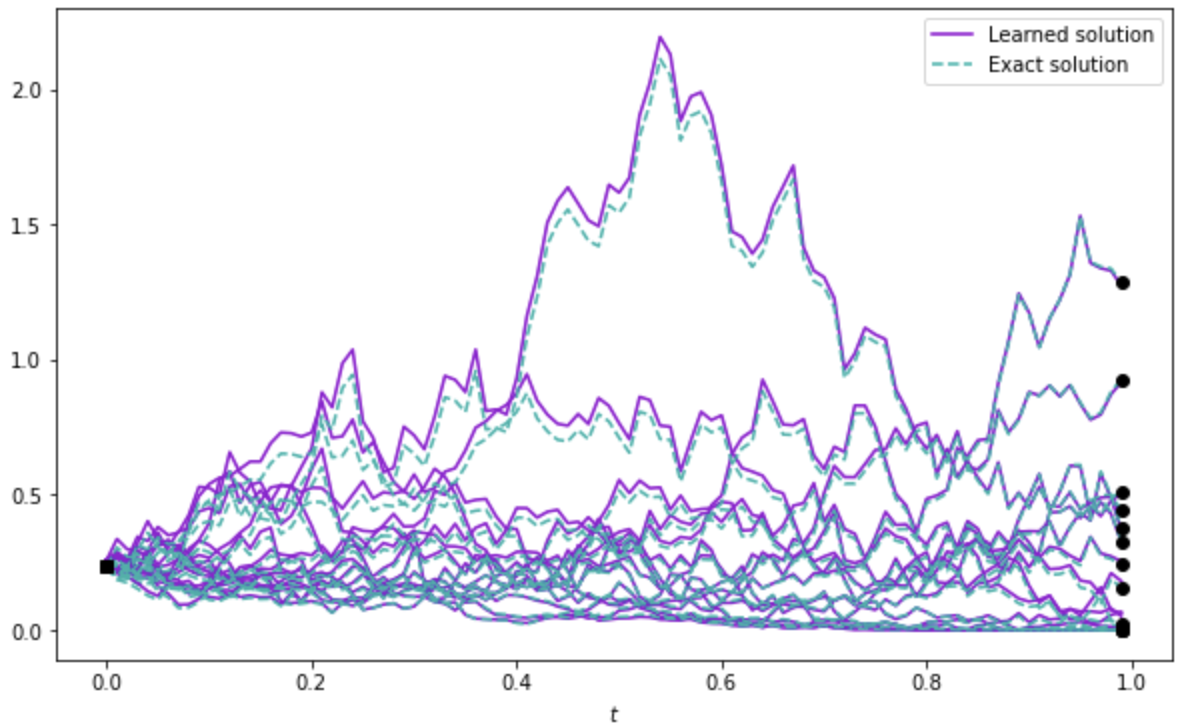
\includegraphics[width = 0.43\textwidth]{GBM_European_price.png}}
	   \quad
    	\subfigure[GBM European  $d=10$]{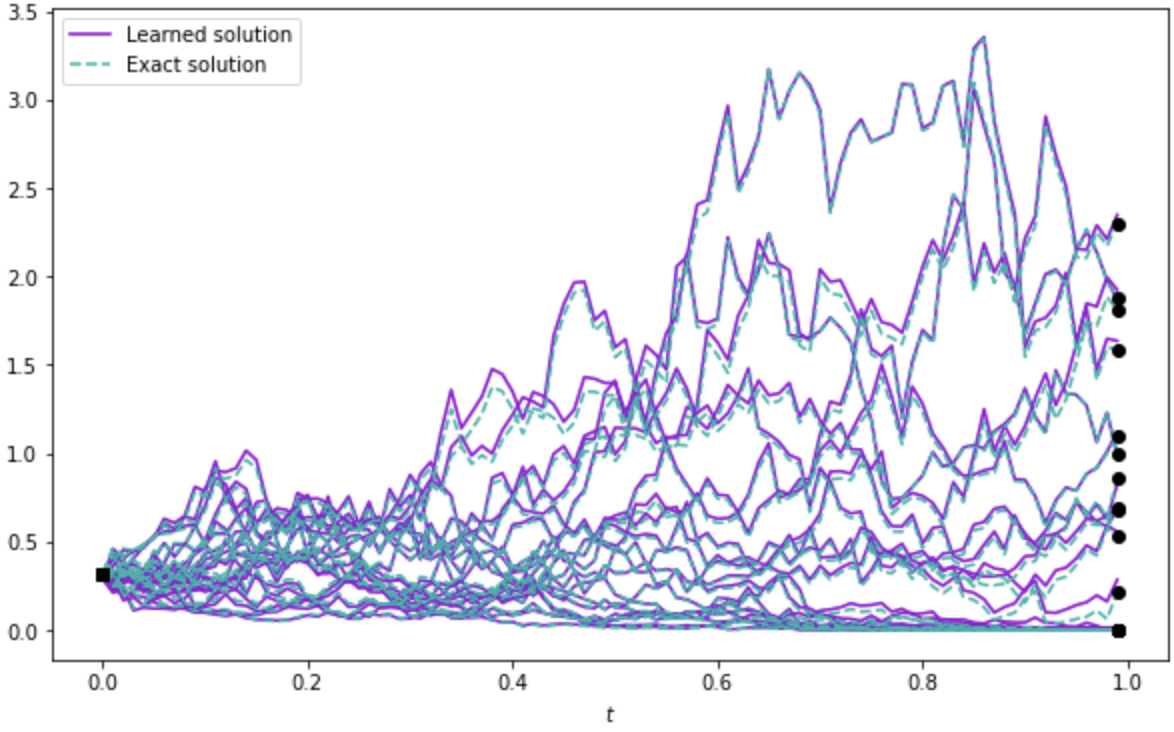
\includegraphics[width = 0.43\textwidth]{GBM_Basket_10.png}}
	    \\
		\subfigure[GBM Lookback ]{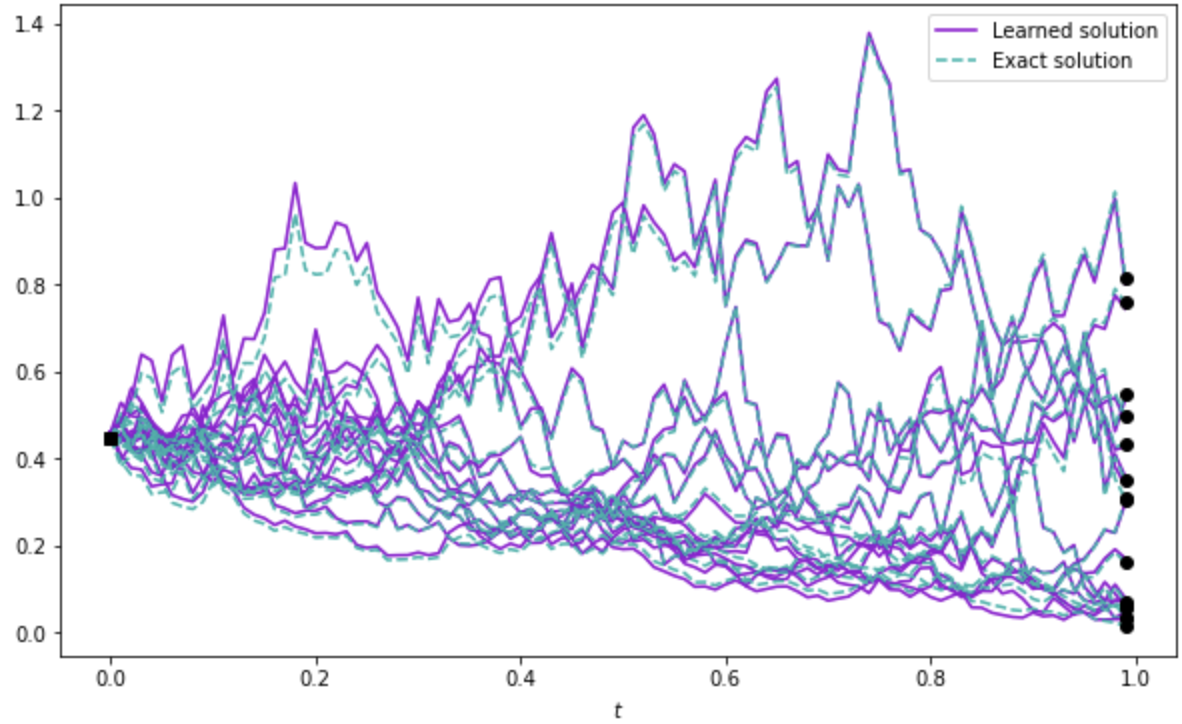
\includegraphics[width = 0.43\textwidth]{GBM_lookback_price.png}}
		\quad
		\subfigure[GBM Asian ($d=1$)]{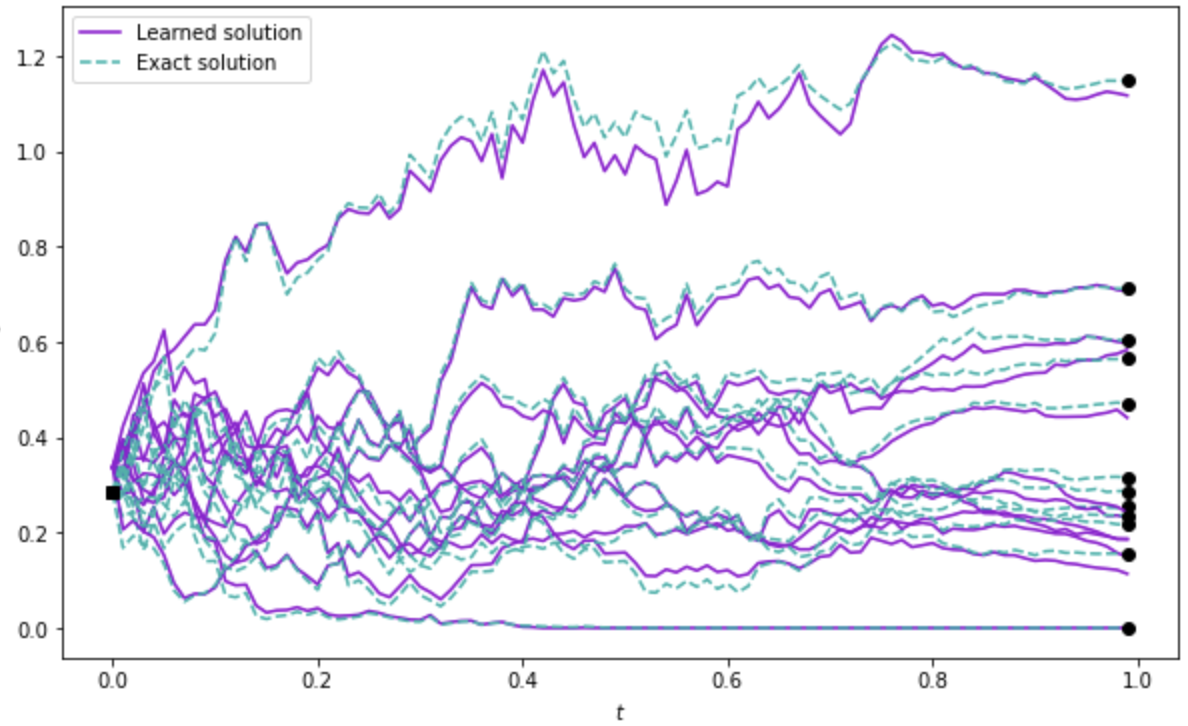
\includegraphics[width = 0.43\textwidth]{GBM_Asian_price.png}}
		\\
		\subfigure[Heston forward $d=1$]{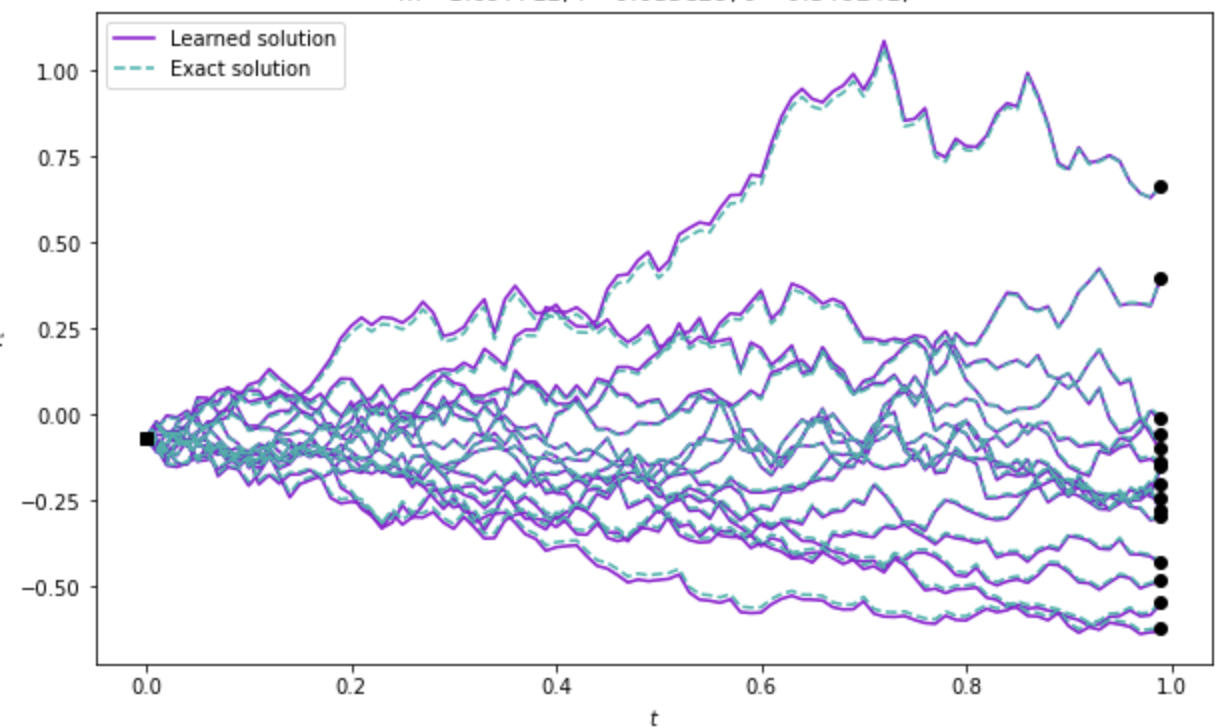
\includegraphics[width = 0.43\textwidth]{SV_forward_price.png}}
		\quad
		\subfigure[Heston forward $d=10$]{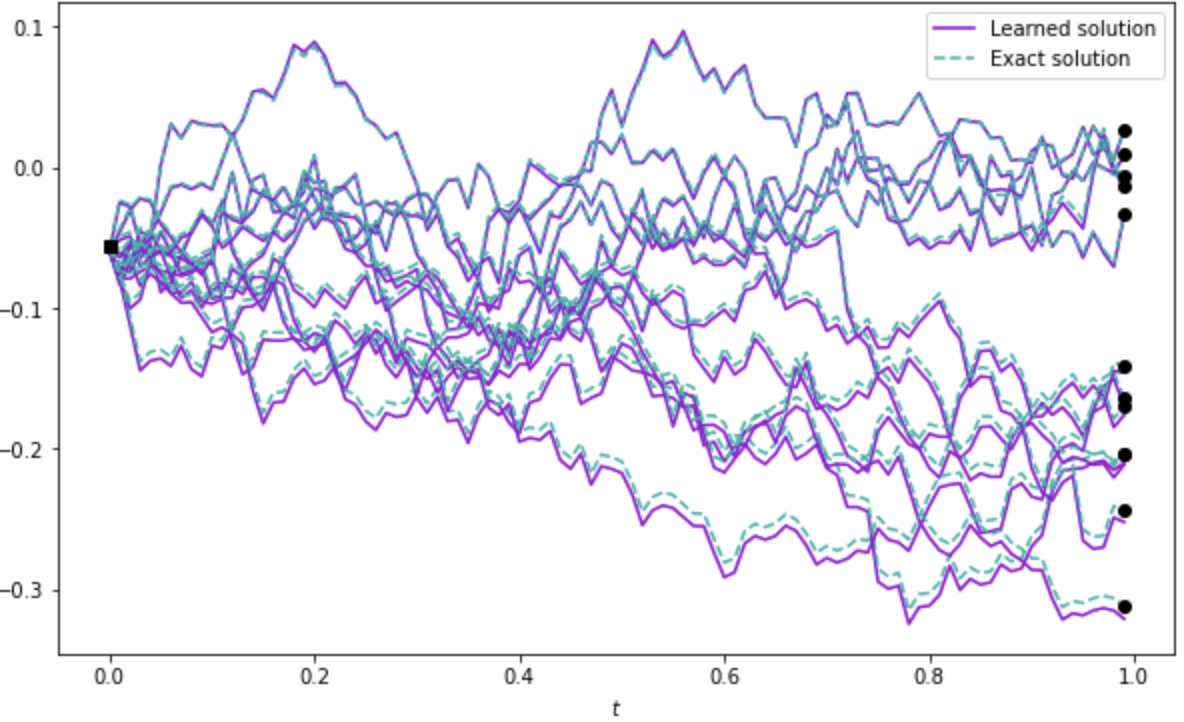
\includegraphics[width = 0.43\textwidth]{SV_forward_10.png}}
		\\
		\caption{Analytical price and predicted price by PONet under the time dependent GBM model and Heston stochastic volatility model. For each subplot, the purple curves are simulated derivative paths from the learned operator network and we legend this as learned solution while the light blue curves are corresponded to analytical solutions.}
		\label{fig:simul-GBM}
	\end{figure}
	\iffalse
	For time-dependent GBM, we set $r_0 = 0.04$, $r_1 = 0.002$, $r_2 = 0.006$, $\bar{\sigma}=0.55$, $\beta=0.03$, $\kappa=0.95$, and $\rho_S=0.14$ for simulation. For Heston stochastic volatility model,  we set $r=0.04$, $\theta = 0.55$, $\alpha_i = 0.13$, $\sigma_i=0.017$, $\rho_S=0.3$, and $\rho_{S,V} = -0.47$ for simulation
	
	\fi
	
	
	
	
	
	
	
	
	
	
	
	
	
	
	
	
	
	
	\iffalse
	
	Thanks to \cite{tensorflow2015-whitepaper}, we can implement our idea with deep learning framework in tensorflow. Our experiments are conducted in two parts. In the first part, we price financial derivatives under the Geometric Brownian Motion (GBM) model and Heston model for both single and multiple dimensions. For time-dependent GBM model, we discretize the time-dependent function and input it into a time grid with 20 uniform sensors on the time horizon of $[0, T]$. We also input the interest rate, $r(t)$, and volatility, $\sigma_i(t), i=1,\cdots,d$, into the branch network with discretization (We also try inputing functions into CNN operator and we also illustrate the results.). To test the model against analytical solutions, we set these functions as constant functions, but they are also discretized to follow the rule of inputting time-varying functions. For the functions input, we first generate a batch of parameters related to functions and then calculate the values on the grid of the domain and input them into branch net. We also use some other approches to input functions such as convolutions and Fourier transformations. In the second part of the experiment, we discuss pricing under the stochastic volatility model using the time-dependent Heston model. The relevant functions here are $r(t)$ and $\theta_i(t), i=1,\cdots,d$. We also use some flat functions to test the result with some basic analytical solutions. We compare the numerical solution with the true solution and calculate the error using absolute error (AE) calculated as $|\mathcal{G}(a_i)(t_n, X_{t_n}) - G_{\theta}(\Tilde{a}_i)(t_n, X_{t_n})|$: at each $(t, x)$ pair and each input function $a_i$. Then we care about the mean and standard deviation.
	
	
	Before delving into the specifics of our experiments, we will first provide an overview of our network structure. Our network consists of two parts: the branch net and the trunk net. For both nets, we specify the width and number of layers for the feedforward neural network (FNN) component. Additionally, for the branch net, we provide the hyperparameters of filters and strides for the convolutional layers. For the trunk net, we specify the width and depth of the componentwise feed forward network of the permutation invariant layer. The details of feed forward layers in DNN of branch and trunk nets as scheduled as follows:
	\begin{itemize}
		\item We initialize the parameters using Xavier initialization (\cite{glorot2010understanding}), which can prevent initial weights in a deep network from being either too large or too small. This method sets the weight of the $j$-th layer to follow a uniform distribution given by 
		\begin{equation}	
			W^{j} \sim U\left[-\frac{1}{\sqrt{n_{j}}}, \frac{1}{\sqrt{n_{j}}}\right], 
		\end{equation}
		where $n_j$ is the number of neurons on the $j$-th layer. 
		
		\item We use the Adam optimizer (\cite{kingma2014adam}) to minimize the loss function.  Calculating the gradient of the loss function using all the samples can be computationally expensive. Therefore, in each iteration, we only use a batch of samples for the gradient evaluation. The shape of a batch of data is $[B, M, N, d+1]$, where $B$ is the batch size of sampled coefficients, $M$ is the number of paths generated under each scenario, $N$ is the time steps on the time horizon, $d$ is the number of assets while another one dimension is for time. The Adam optimizer is a popular gradient-descent algorithm, which utilizes the exponentially weighted average of the gradients to accelerate convergence to the minimum. 
		
		\item We apply batch normalization to the inputs of the neural network (\cite{ioffe2015batch}). For all the samples in a batch, we first estimate the mean and standard deviation of each input in this batch. Then, we normalize the input by subtracting its estimated mean and dividing by its estimated standard deviation. 
		
	\end{itemize}
	
	\begin{table}[htbp]
		\centering
		\begin{tabular}{ccc}
			\hline
			network  & single dimension & multi-dimension \\
			\hline  
			Branch net &  $[15, 15, 15]$  & $[15, 15, 15, 15]$  \\
			Trunk net& $[15, 15, 15]$  & $[15, 15, 15, 15]$  \\
			
			Embedding net& $[20, 20]$ & $[20, 20]$  \\
			PI net& $[10, 10]$  & $[15, 15]$  \\
			\hline
		\end{tabular}
		\caption{Structure of PONet in single and multi-dimensional cases}
		\label{tab:structure1}
	\end{table}
	
	Next, we provide an overview of our training settings for the experiments. We use the Adam optimizer with a learning rate of 0.005 and iterate for 1000 steps for each experiment. For each step, we draw a batch of coefficients from a distribution, which will be discussed later.
	
	For each batch of coefficients, we simulate several sample paths, denoted by the sample size. The sample size is shown in the table below:
	\begin{table}[htbp]
		\centering
		\begin{tabular}{cc}
			\hline		
			hyper-parameter & value \\
			\hline   optimizer &Adam \\
			learning rate & 0.005\\
			$B$ (train) & 200\\
			$B$ (test) & 100\\
			$M$ (train) & 50\\
			$M$ (test) & 30\\
			\hline
			
			
		\end{tabular}
		\caption{Setting of training and testing}
		\label{tab:training setting}
	\end{table}
	
	To test the accuracy of our model, we sample a smaller batch of coefficients from a distribution with a range half as narrow as that used in the training process. The details of this distribution will be discussed later. We select the midpoint of the interval and generate a series of paths, from which we derive the option value and corresponding coefficients. For better accuracy of the option prices conditioned on the coefficients which live in the desired parameter range, we train the operator by sampling parameters related to functions in a distribution wider range. Then we make comparisons between the MAE over the whole region and MAE error over the central region.
	\subsection{European and Exotics under Time Dependent GBM}
	we test the case under time dependent GBM again on non constant functions. The interest rate functions $r(t)$ is parameterized by:
	\begin{equation*}
		r(t) =r_0 + r_1 t + r_2 t^2
	\end{equation*}
	The volatility function is parameterized by 
	\begin{equation*}
		\sigma_i(t) = (\sigma_0)_i e^{-\beta_i (T - t)}, i=1,\cdots,d
	\end{equation*}
	Then we train the operator network with input of this time-dependent interest rate function. Before that, we show several analytical solutions under time dependent GBM (strike price is expressed as $K =S_0 \cdot k$).
	
	
	\noindent Details about the product payoffs are provided in Section 3.1. In this section, we train a European call option operator under multiple dimensions. For the path simulation under multi-dimensional case, we let the correlations between any two of assets are same and we denote this as $\rho_S$. The coefficients used for training and validation are sampled as follows:
	\begin{table}[H]
		\centering
		\caption{input function parameter sampling under Heston model}
		\begin{tabular}{ccc}
			\hline
			$\text{parameter}$    &   dist. (whole) & dist. (central) \\
			\hline
			$r_0$   & $U(0.005, 0.08)$  &  $U(0.025, 0.65)$\\
			$r_1$   & $U(0.001, 0.004)$  &  $U(0.0015, 0.0035)$\\
			$r_2$   & $U(0, 0.01)$  &  $U(0.001, 0.008)$\\
			$(\sigma_0)_i, i=1\cdots,d$   & $U(0.2, 0.8)$  &  $U(0.3, 0.7)$\\
			$(\beta)_i, i=1\cdots,d$   & $U(0.01, 0.04)$  &  $U(0.02, 0.03)$\\
			$\rho_S$  & $U(-\frac{1}{d}, 0.8)$ & $U(-\frac{1}{d}+0.1, 0.6)$  \\
			$\textit{k}$ & $N(1.0, 0.2)$ & $N(1.0, 0.1)$\\
			\hline
			
		\end{tabular}%
		\label{tab:dists}%
	\end{table}%
	Then we show the mean and standard deviation of absolute error (AE) under whole region and central region as following table:
	\begin{table}[H]
		\centering
		\begin{tabular}{cccccc}
			\hline$d$ & iteration & $\begin{array}{c}\text{AE(whole)} \\
				\text{mean (std.)} \end{array}$   & $\begin{array}{c}\text{AE(central)} \\
				\text{mean (std.)} \end{array}$  \\
			\hline \multirow{4}{*}{1} & 100 & 0.3631 (0.1980) & 0.2893 (0.2473) \\
			& 200 & 0.0386  (0.0477) & 0.0438 (0.0371) \\
			& 500 & 0.0272 (0.0237) & 0.0199 (0.0201) \\
			& 1000 & 0.0213 (0.0207) & 0.0167  (0.0114) \\
			
			\hline \multirow{4}{*}{5} & 100 & 0.3128 (0.1736) & 0.1829 (0.1900) \\
			& 200 & 0.0575 (0.0426) & 0.0483 (0.0390) \\
			& 500 & 0.0355 (0.0350) & 0.0211 (0.0183) \\
			& 1000 & 0.0331 (0.0336) & 0.0202 (0.0176) \\
			
			\hline \multirow{4}{*}{10} & 100 & 0.2182 (0.1928) & 0.1776 (0.1065) \\
			& 200 & 0.0486 (0.0414) & 0.0477 (0.0273) \\
			& 500 & 0.0355 (0.0249) & 0.0417 (0.0193) \\
			& 1000 & 0.0278 (0.0214) & 0.0218 (0.0169) \\
			
			% \hline \multirow{4}{*}{20} & 100 & 0.4776 & 0.2817 & 0.4288 & 0.2736 \\
			%                         & 200 & 0.0759 & 0.0663 & 0.0528 & 0.0433 \\
			%                         & 500 & 0.0472 & 0.0359 & 0.0277 & 0.0230 \\
			%                         & 1000 & 0.0327 & 0.0304 & 0.0209 & 0.0167 \\
			\hline \multirow{4}{*}{GBM-Lookback} & 100 & 0.2586 (0.2006) & 0.1726 (0.2473) \\
			& 200 & 0.0364 (0.0418) & 0.0289 (0.0247) \\
			& 500 & 0.0295 (0.0236)  & 0.0218 (0.0191) \\
			& 1000 & 0.0235 (0.0207) & 0.0212 (0.0210) \\
			
			\hline \multirow{4}{*}{GBM-Asian} & 100 & 0.3081 (0.1736) & 0.2812 (0.1635) \\
			& 200 & 0.0563 (0.0426) & 0.0322 (0.0314) \\
			& 500 & 0.0417 (0.0398) & 0.0279 (0.0288) \\
			& 1000 & 0.0368 (0.0355) & 0.0211 (0.0193) \\
			
			\hline
		\end{tabular}
		\caption{results of Time dependent GBM European options: Compare the error sampling from whole function domain and central domain. While first three sub-tables shows the result of European options and last two tables show the look back and Asian}
		\label{tab:my_label}
	\end{table}
	We also give the result table on arithmetric basket call option but we just compare the result at the initial time since nest Monte Carlo is time consuming. The result is as follows:
	\begin{table}[H]
		\centering
		\begin{tabular}{cccccc}
			\hline$\text{SDE-product}$ & iteration & $\begin{array}{c}\text{AE(whole)} \\
				\text{mean (std.)} \end{array}$   & $\begin{array}{c}\text{AE(central)} \\
				\text{mean (std.)} \end{array}$  \\
			\hline \multirow{4}{*}{GBM-Arithmetic Basket} & 100 & 0.2586 (0.2006) & 0.1726 (0.2473) \\
			& 200 & 0.0364 (0.0418) & 0.0289 (0.0247) \\
			& 500 & 0.0295 (0.0236)  & 0.0238 (0.0191) \\
			& 1000 & 0.0248 (0.0202) & 0.0211 (0.0179) \\
			
			
			\hline
		\end{tabular}
		
		\caption{results of time-dependent GBM arithmetric basket options}
		\label{tab:my_label}
	\end{table}
	Then We give the curve comparison between the learned values and values yield from analytical solution
	\begin{figure}[H]
		\centering
		\subfigure[BS price $d=1$]{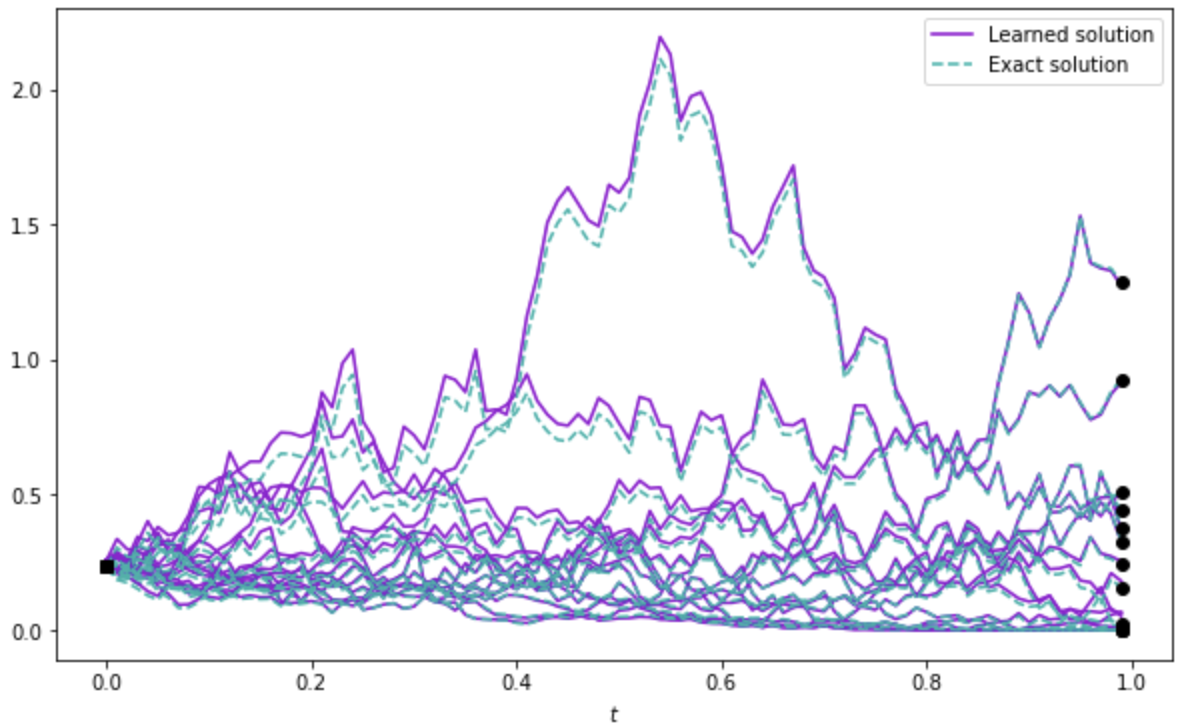
\includegraphics[width = 0.4\textwidth]{GBM_European_price.png}}
		\quad
		\subfigure[BS price $d=10$]{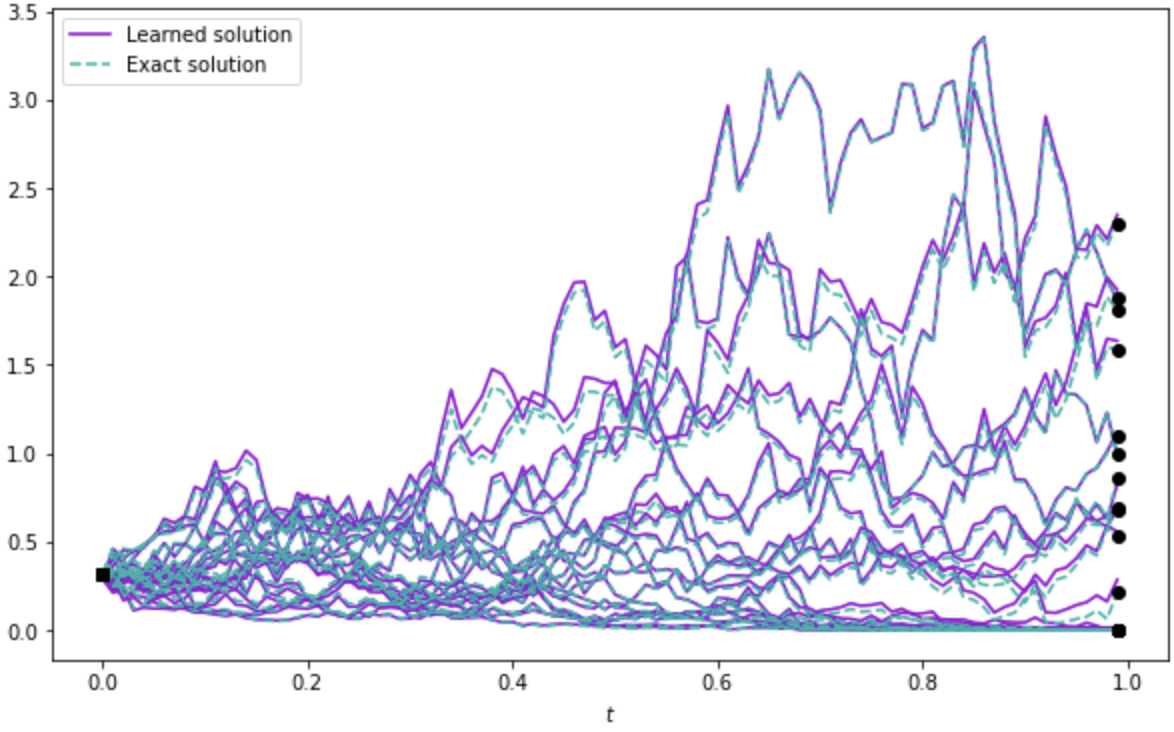
\includegraphics[width = 0.4\textwidth]{GBM_Basket_10.png}}
		\\
		\subfigure[Lookback price]{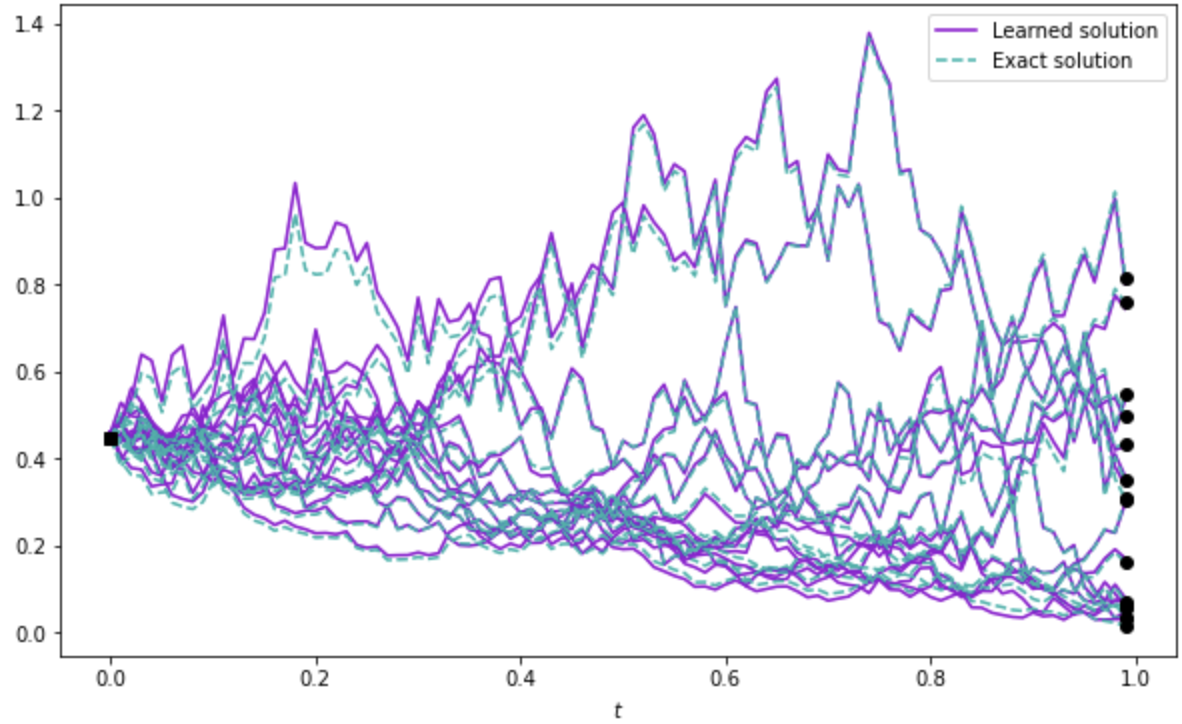
\includegraphics[width = 0.4\textwidth]{GBM_lookback_price.png}}
		\quad
		\subfigure[Asian price]{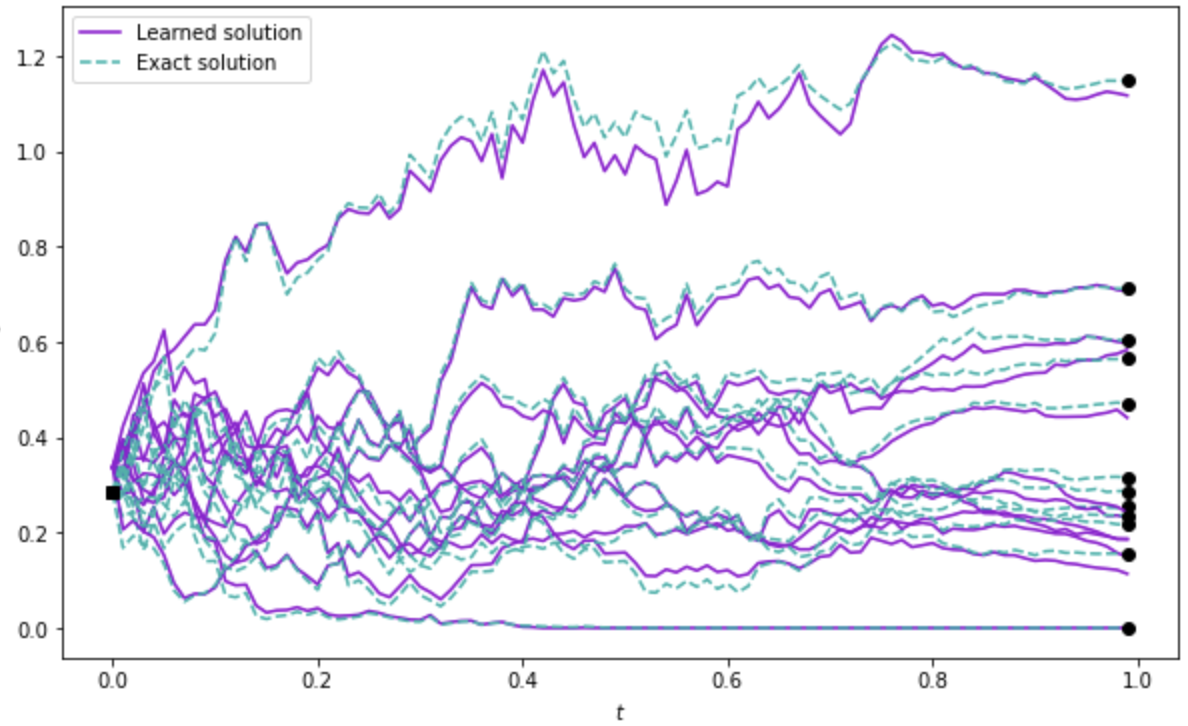
\includegraphics[width = 0.4\textwidth]{GBM_Asian_price.png}}
		
		\caption{Analytical price and predicted price under GBM, the asset price is generated with $r = 0.04$, $\sigma_i = 0.5$ and $k = 1.01$. (a) and (b) shows the comparison under $d=1$ and $d=10$ European options while (c) shows the lookback option and (d) shows Asian option.}
		\label{fig:GBM call}
	\end{figure}
	In the GBM cases table, we observe that the absolute error consistently converges under different dimensions. The loss function and absolute error reach a relatively low level after the first 500 steps. When we compare results horizontally, we find that the operator achieves a lower mean error and standard deviation when we sample from the central part of the distribution $\mu$. This suggests that inferring on a domain with denser density of distribution can enhance accuracy. For path dependent options, the results are similar. For the Asian option, the error is slightly larger than in the European cases. However, we see from the curve that the operator converges to the analytical solution. Due to the complexity of the payoff structure (without the state variable), the delta is not explicit enough for the value network to learn as time approaches maturity. Thus, we need to consider the zero-delta constraint at the terminal payoff.
	
	\subsection{Heston Model}
	Under heston model, besides the rate function, we care about the mean reversion function $\theta(t)$ and we parameterize it with:
	\begin{equation*}
		\theta_i(t) = (\theta_0)_i e^{-\gamma_i (T - t)}, i=1,\cdots,d
	\end{equation*}
	This function has the same parameterization with the time dependent GBM case since it is assumed that the volatility under that dynamics has no stochastic noise around the mean level.
	For the convenience of testing with analytical solutions, we choose the forward as the product and the fair value is:
	\begin{equation*}
		u(t, S_t, V_t;a) = \frac{1}{d}\sum_{i=1}^d S^i_t - K e^{-\int_t^T r(s)ds}
	\end{equation*}
	Since it is a delta one product, the hedging ratio is just $\sqrt{V_t}S_t$ and $K = S_0 \cdot k$.
	For multi dimensional Heston model, one issue is the correlation matrix of the vector of assets and their corresponded volatilities. The correlation matrix $\Sigma$ is of the form:
	\begin{equation*}
		\Sigma=\left(\begin{array}{cc}
			\Sigma_S & \Sigma_{S V} \\
			\Sigma_{S V}^{\top} & I_d
		\end{array}\right)
	\end{equation*}
	with $I_d$ the $d \times d$-identity matrix, $\Sigma_S$ the $d \times d$-correlation matrix of the stocks, and $\Sigma_{S V}$ a diagonal matrix of the same size, given by:
	\begin{equation*}
		\Sigma_{S V}=\left(\begin{array}{cccc}
			\rho_V & 0 & \ldots & 0 \\
			0 & \rho_V & \ldots & 0 \\
			\vdots & \vdots & \ddots & 0 \\
			0 & 0 & 0 & \rho_V
		\end{array}\right)
	\end{equation*}
	
	
	\begin{table}[H]
		\centering
		\caption{input function parameter sampling under Heston model}
		\begin{tabular}{ccc}
			\hline
			$\text{parameter}$    &   dist. (whole) & dist. (central) \\
			\hline
			$r$   & $U(0.005, 0.08)$  &  $U(0.025, 0.65)$\\
			$(\theta_0)_i, i=1\cdots,d$   & $U(0.09, 1.20)$ & $(0.3, 0.9)$\\
			$(\gamma_i, i=1\cdots,d$   & $U(0.0001, 0.001)$ & $(0.0003, 0.0009)$\\
			$\kappa_i, i=1\cdots,d$  & $U(0.05, 0.25)$ & $U(0.1, 0.15)$\\
			$\sigma_i, i=1\cdots,d$  & $U(0.001, 0.003)$ & $U(0.015, 0.02)$\\
			$\rho_S$  & $U(-\frac{1}{d}, 0.8)$ & $U(-\frac{1}{d}+0.1, 0.6)$  \\
			$\rho_V$  & $U(-0.8, 0.1)$  & U(-0.5, 0.01) \\
			$\textit{k}$ & $N(1.0, 0.2)$ & $N(1.0, 0.1)$\\
			\hline
			
		\end{tabular}%
		\label{tab:dists}%
	\end{table}%
	Then we have the error table under different dimension
	
	
	\begin{table}[H]
		\centering
		\begin{tabular}{cccccc}
			\hline$d$ & iteration & $\begin{array}{c}\text{AE(whole)} \\
				\text{mean (std.)} \end{array}$   & $\begin{array}{c}\text{AE(central)} \\
				\text{mean (std.)} \end{array}$  \\
			\hline \multirow{4}{*}{1} & 100 & 0.3115 (0.2673) & 0.2956 (0.2473) \\
			& 200 & 0.0386 (0.0358) & 0.0238 (0.0271) \\
			& 500 & 0.0261 (0.0207) & 0.0191 (0.0200) \\
			& 1000 & 0.0122 (0.0105) & 0.0069 (0.0057) \\
			% \hline \multirow{4}{*}{5} & 100 & 0.2658 & 0.1162 & 0.0987 & 0.0896 \\
			%                         & 200 & 0.0348 & 0.0326 & 0.0212 & 0.0209 \\
			%                         & 500 & 0.0211 & 0.0183 & 0.0177 & 0.0126\\
			%                         & 1000 & 0.0103 & 0.0082 & 0.0063 & 0.0048 \\                      
			\hline \multirow{4}{*}{10} & 100 & 0.2459 (0.1333) & 0.1868 (0.1144) \\
			& 200 & 0.0347 (0.0313) & 0.0227 (0.0210) \\
			& 500 & 0.0215 (0.0189) & 0.0184 (0.0160) \\
			& 1000 & 0.0114 (0.0120) & 0.0075 (0.0061) \\
			
			\hline
		\end{tabular}
		\caption{results of SV forward}
		\label{tab:my_label}
	\end{table}
	The the pricing curve for one dimensional and multiple dimensional forward contract and hedge curve for one dimensional forward is given with following figures:
	\begin{figure}[H]
		\centering
		\subfigure[price $d=1$]{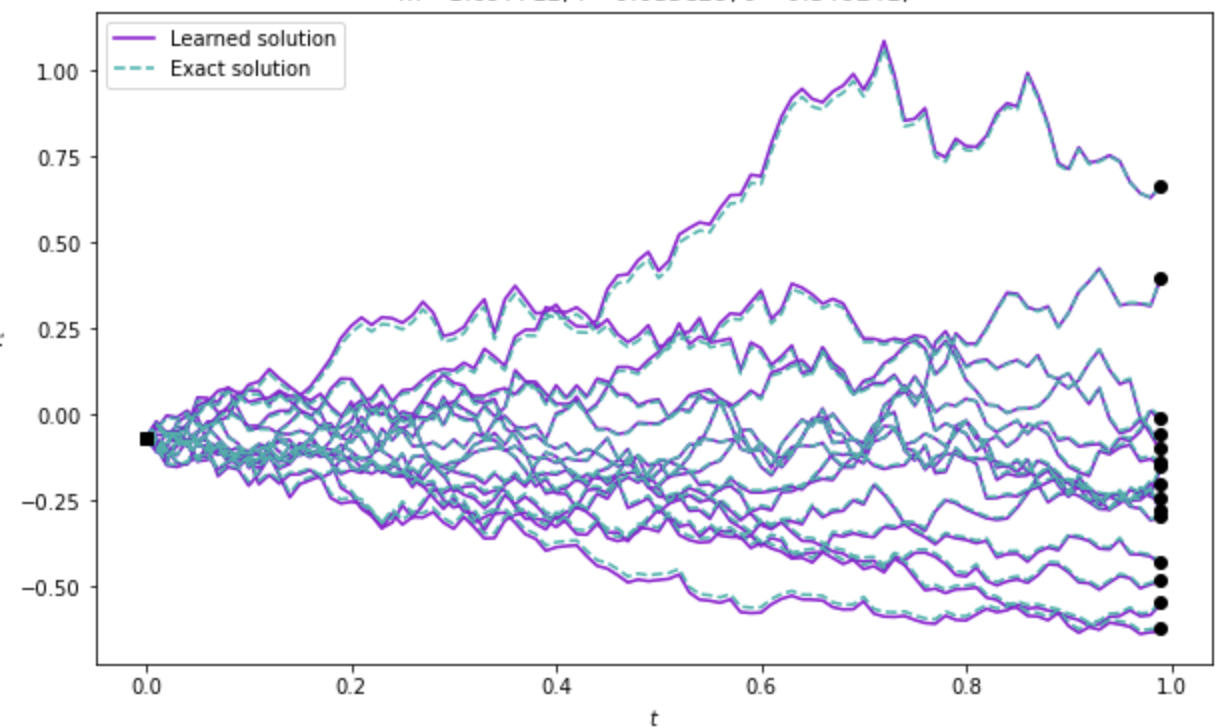
\includegraphics[width = 0.4\textwidth]{SV_forward_price.png}}
		\quad
		\subfigure[price $d=10$]{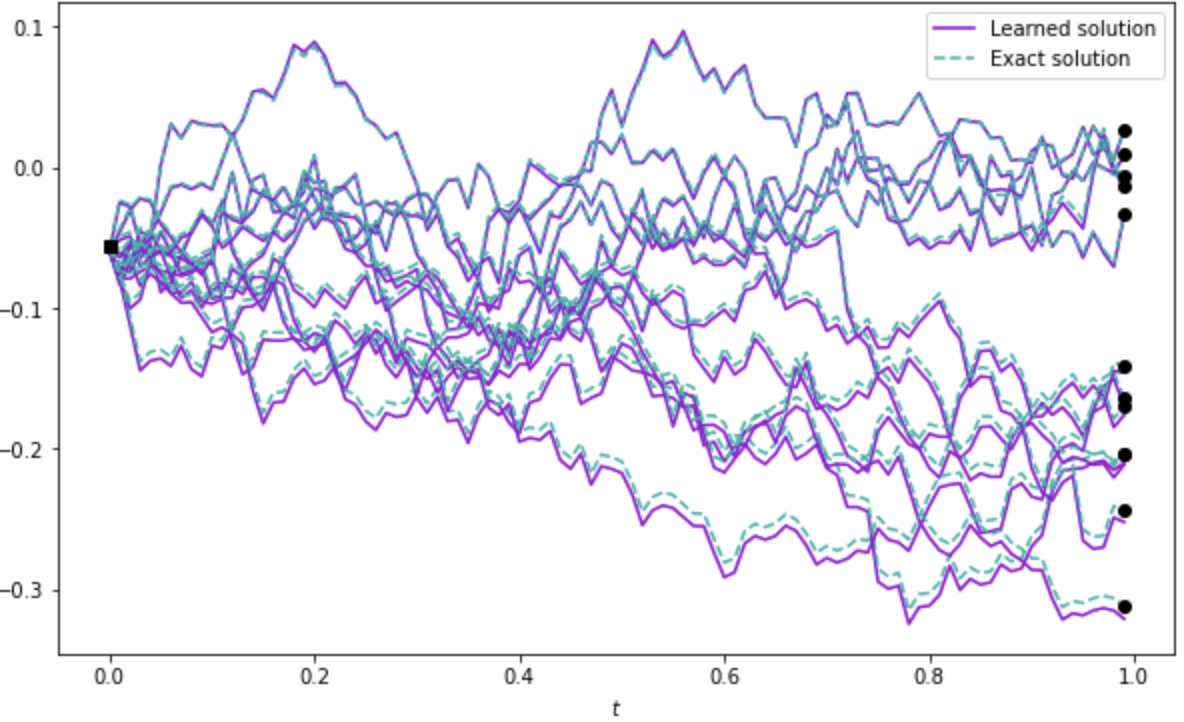
\includegraphics[width = 0.4\textwidth]{SV_forward_10.png}}
		\\
		\caption{price comparison under multiple dimensions comparision under $1-d$ time dependent SV}
		\label{fig:SV forward}
	\end{figure}
	We observe that in the single-dimensional case, the price and hedge process are well-fitted, and in the multi-dimensional case, they are also well-fitted with no significant increase in error. However, training the PricingONet under multi-dimensional cases is more time-consuming, with the time increasing linearly with the dimension. The main reason for this is that, due to the nature of approximating the pricing kernel with only a neural network, the construction of the computational graph is more complex compared to the graph in \cite{han2017deep} and \cite{beck2021deep}, which use only one value network for a single time step with MSE loss as the total loss function. Extending this approach into the operator learning framework will be a topic for future discussion. We also give the result of the arithmetric basket options under time-dependent Heston model in 10 dimensions. Compared with Monte Carlo methods:
	\begin{table}[H]
		\centering
		\begin{tabular}{cccccc}
			\hline$\text{SDE-product}$ & iteration & $\begin{array}{c}\text{AE(whole)} \\
				\text{mean (std.)} \end{array}$   & $\begin{array}{c}\text{AE(central)} \\
				\text{mean (std.)} \end{array}$  \\
			\hline \multirow{4}{*}{SV-Arithmetic Basket} & 100 & 0.6324 (0.3827) & 0.4530 (0.3110) \\
			& 200 & 0.0832 (0.0527) & 0.0677 (0.0499) \\
			& 500 & 0.0492 (0.0332)  & 0.0303 (0.0288) \\
			& 1000 & 0.0315 (0.0233) & 0.0291 (0.0210) \\
			
			
			\hline
		\end{tabular}
		
		\caption{results of arithmetric basket options under time-dependent Heston }
		\label{tab:my_label}
	\end{table}
	\subsection{Permutation Invariant and Different input representation}
	
	\noindent \textbf{PI or without PI}: We compare the PricingONet with and without a permutation invariant ($PI$) layer in a multi-dimensional scenario. For the network without the PI layer, we add two additional feedforward layers with the same width as the trunk net. All training settings remain the same. We then compare the pricing values and summarize the error as following table:
	\begin{table}[htbp!]
		\centering
		\begin{tabular}{cccccc}
			\hline Design & iteration & $\begin{array}{c}\text{AE (whole)} \\
				\text{mean (std.)} \end{array}$   & $\begin{array}{c}\text{AE (central)} \\
				\text{mean (std.)} \end{array}$  \\
			\hline \multirow{4}{*}{With PI ($d=10$)} & 100 & 0.2182 (0.1928) & 0.1776 (0.1065) \\
			& 200 & 0.0486 (0.0414) & 0.0277 (0.0273) \\
			& 500 & 0.0255 (0.0249) & 0.0217 (0.0193) \\
			& 1000 & 0.0228 (0.0214) & 0.0188 (0.0129) \\ 
			\hline \multirow{4}{*}{Without PI ($d=10$)} & 100 & 0.2591 (0.1210) & 0.1972 (0.1107) \\
			& 200 & 0.0476 (0.0408) & 0.0319 (0.0323) \\
			& 500 & 0.0392 (0.0365) & 0.0287 (0.0250) \\
			& 1000 & 0.0345 (0.0264) & 0.0221 (0.0174) \\
			\hline
		\end{tabular}
		\caption{Comparison of two designs under the time-homogeneous GBM model for the European geometric basket call option}
		\label{tab:comp-PI}
	\end{table}
	
	We observe that the network without a PI layer has worse performance, as it takes longer to converge compared to the network with a PI layer. In contrast, the network with a PI layer performs significantly better, and we can clearly see a good fit with the analytical solution. The main reason for this is that the permutation invariant structure ensures that the number of parameters in the first two layers remains the same as in the one-dimensional case, and does not increase as the dimension increases. However, an issue that is not considered in this framework is that the input coefficients related to each asset should also be permutation invariant theoretically. Here are two possible solutions for this issue: Firstly, look for some interactions between the branch net and trunk net. Secondly, do parameterizations on some coefficients, such as correlation matrices, to reduce the dimension to $\mathbb{R}^d$ rather than $\mathbb{R}^{d \times d}$, which can then be inputted into the trunk net as constant values. However, for operator inference, if we do not do extra permutation for multi-assets, it is sufficient to equip only the trunk net with permutation invariant property.
	
	
	\noindent \textbf{different input representation method}: we test the case under time dependent GBM again using different input function embdding methods
	Then we have the following results with figure:
	\begin{figure}[h!]
		\centering
		\subfigure[Fourier]{\includegraphics[width = 0.4\textwidth]{TGBM_TimeEuropean_rs_dense.png}}
		\quad
		\subfigure[conv]{\includegraphics[width = 0.4\textwidth]{TGBM_TimeEuropean_rs_conv.png}}
		\caption{}
		\label{fig:path}
	\end{figure}
	
	We also give the comparison of error on whole input domain and central domain:
	\begin{table}[H]
		\centering
		\begin{tabular}{cccccc}
			\hline$d$ & iteration & $\begin{array}{c}\text{AE(whole)} \\
				\text{mean (std.)} \end{array}$   & $\begin{array}{c}\text{AE(central)} \\
				\text{mean (std.)} \end{array}$  \\
			\hline \multirow{4}{*}{dense} & 100 & 0.3883 (0.2613) & 0.2966 (0.2550) \\
			& 200 & 0.1292 (0.0955) & 0.1001 (0.0821) \\
			& 500 & 0.0600 (0.0431) & 0.0422 (0.0388) \\
			& 1000 & 0.0315 (0.0287) & 0.0284 (0.0205) \\                
			\hline \multirow{4}{*}{conv} & 100 & 0.4261 (0.3551) & 0.4587 (0.3241) \\
			& 200 & 0.1367 (0.0997) & 0.0965 (0.0723) \\
			& 500 & 0.0583 (0.0369) & 0.0514 (0.0377) \\
			& 1000 & 0.0252 (0.0215) & 0.0226 (0.0162) \\
			\hline \multirow{4}{*}{Fourier} & 100 & 0.2283 (0.1982) & 0.1997 (0.1252) \\
			& 200 & 0.0348 (0.0326) & 0.0212 (0.0209) \\
			& 500 & 0.0211 (0.0183) & 0.0177 (0.0126)\\
			& 1000 & 0.0283 (0.0182) & 0.0255 (0.0198) \\ 
			
			\hline
		\end{tabular}
		\caption{results of time dependent GBM: We compare the performance under time dependent GBM under three methods to embedding functions: 1. Straightforwardly input discretized functions into the FNN. 2. Using convolution network to  embed the function into frequency domain. 3. Using Fourier transformation to get Fourier modes}
		\label{tab:my_label}
	\end{table}
	
	
	
	
	
	\fi
	
	
	
	
	
	
	
	
	
	
	
	
	
	
	
	
	\subsection{Fixed-Income Products}
	In Hull-White model, we initialize the forward rate curve with the flatten curve, and there is a constraint that  $\theta_r = R_0$.  We also input the curve into operator network as a function. Then the table \ref{tab:dist-HW} gives the distribution of parameters:
	\begin{table}[htbp!]
		\centering
		\begin{tabular}{ccc}
			\hline
			$\text{parameter}$    &   distribution  \\
			\hline
			$\theta(t) = R_0$   & $U(0.04, 0.06)$ \\
			$\kappa$  & $U(0.3, 0.5)$ \\
			$\sigma$  & $U(0.02, 0.04)$ \\
			\hline
		\end{tabular}%
		\caption{Sampling distributions of coefficients under the Hull White model: The equation $\theta(t) = R_0$ means that there is a constrain in HW model and then we just need to only sample $\theta$ rather than sample both $\theta$ and $R_0$. Since we let the rate curve become flat, we just need to sample $\theta = \theta(t)$ in a uniform distribution.}
		\label{tab:dist-HW}%
	\end{table}%
	\subsubsection{Zero Coupon Bond}
   Since the bond price $P(t, T)$ is the most crucial component in the payoff structure of almost every fixed income instrument. We begin by testing the price of a zero-coupon bond  $P(t, T)$, which can be considered as a special case where the strike of a bond option is zero. In this case, the dynamics of the zero-coupon bond follow the Heath-Jarrow-Morton (HJM) model. For a bond with maturity $T$, we have the following Backward Stochastic Differential Equation (BSDE):
   \begin{align*}
   	d P(t, T) &= R_t P(t, T) dt + \sigma B(t, T)P(t, T) d W_t \\
   	P(T, T) &= 1
   \end{align*}
   where $	B(t, T)=\frac{1-e^{-a(T-t)}}{a}$. Then plug this into our European framework. We can yield the result as following plot, which is a comparison between analytical solution and value given by operator:
   \begin{figure}[h!]
   	\centering
   	\includegraphics[scale=0.16]{zcp.jpg}
   	\caption{result of zero coupon bond. We can find the the learned solution converge to the analytical solution and the initial value and interiors value both come close to the path of analytical solution.}
   	\label{fig:zcp}
   \end{figure}
	
\subsubsection{Bermudan Swaption}
	Building upon the successful results obtained thus far, we proceed with the testing of the Bermudan swaption. For data, we sample coefficients of Hull-White model under the same distribution as in \ref{tab:dist-HW}. Then we list the elements of the Bermudan swaption of interest as following table.
		\begin{table}[htbp]
		\centering
		\begin{tabular}{cc}
			\hline
			item&value  \\
			\hline
			expiry date & 1y \\
			maturity date & 3y \\
			swap increment & 1y \\
			exercise date & 1y, 2y\\
			\hline
			
		\end{tabular}
	\end{table}
	
	
	To establish a benchmark for evaluation, we utilize the numerical solution provided by the \texttt{tf\_quant\_finance} library. We evaluate the initial price of the swaption at various states and parameters, comparing them to the benchmark to assess the level of closeness. For these experiments, we set the fixed rate as zero and the product is equivalent as the swap rate. Then we change the volatility and report the result again.
	\begin{table}[htbp]
		\centering
		\begin{tabular}{cccc}
			\hline
			$\sigma$&$\theta_r = r_0$  & price from operator & benchmark \\
			\hline
			\multirow{5}{*}{0.03} &0.052 & 0.0846  & 0.0901 \\
			&0.053 & 0.0854  & 0.0917 \\
			&0.055 & 0.0872  & 0.0949 \\
			&0.057 & 0.0888  & 0.0982 \\
			&0.058 & 0.0896  & 0.0997 \\
			\hline  
			\multirow{5}{*}{0.05} & 0.052 & 0.0846  & 0.0835 \\
			&0.053 & 0.0854  & 0.0851 \\
			&0.055 & 0.0872  & 0.0885 \\
			&0.057 & 0.0884  & 0.0917 \\
			&0.058 & 0.0897  & 0.0933 \\
			\hline
			
		\end{tabular}
		\caption{Result of the Bermudan Swaption price comparison with $\kappa=0.4$ and $\sigma=[0.03, 0.05]$. The first colume give the level of the flatten forward rate curve at initial time; The second colume (price from operator) gives the price of Bermudan Swaption calculated from the trained operator at initial time; The third colume is the same price given by the benchmark from \texttt{tf\_quant\_finance} library}
		\label{tab:BSwaption1}
	\end{table}
	From \ref{tab:BSwaption1}, We observe that as the input parameter approaches the sample boundary, the magnitude of the error increases significantly. Furthermore, the operator demonstrates the capability to learn the relationship between price and volatility, exhibiting monotonic behavior. 
	
 Another test to assess the Bermudanarity of the swaption involves substituting the analytical solution with the continuation value of the last sub-time interval \footnote{We just substitute the continuation value in the last exercise period into the analytical ones since only in the last time period does it have analytical value which is the European swaption or Bond option}. Since the continuation value of the final time interval corresponds to the European swaption, which possesses a closed-form solution, this approach effectively eliminates the error introduced by the terminal condition. Consequently, we can examine whether the resulting error is smaller than the benchmark or not. The price yield from the analytical continuation value is denoted as price (cont. from ana.) while the price from the last network inference is denoted as  price (cont. from net).
	\begin{table}[htbp]
		\centering
		\begin{tabular}{ccccc}
			\hline
			$\sigma$&$\theta_r = R_0$  & price (cont. from net) & price (cont. from ana.) &benchmark \\
			\hline
			\multirow{5}{*}{0.03} &0.052 & 0.0846 & 0.0875 & 0.0901 \\
			&0.053 & 0.0854 & 0.0883  & 0.0917 \\
			&0.055 & 0.0872  & 0.0901 & 0.0949 \\
			&0.057 & 0.0888  & 0.0920 & 0.0982 \\
			&0.058 & 0.0896  & 0.0927 & 0.0997 \\
			\hline  
			\multirow{5}{*}{0.05} & 0.052 & 0.0846 & 0.0875  & 0.0835 \\
			&0.053 & 0.0854 & 0.0884 & 0.0851 \\
			&0.055 & 0.0872  & 0.0902& 0.0885 \\
			&0.057 & 0.0884  & 0.0919& 0.0917 \\
			&0.058 & 0.0897  & 0.0928& 0.0933 \\
			\hline
			
		\end{tabular}
		\caption{The first colume give the level of the flatten forward rate curve at initial time; The second colume (price from operator) gives the price of  Bermudan Swaption calculated from the trained operator at initial time; The third colume gives the  Bermudan Swaption price when the \textcolor{blue}{continuation value of the last exercise period is calculated by analytical solution rather than the neural operator trained from the last time interval} (We just substitute the continuation value in the last exercise period into the analytical ones since only in the last time period does it have analytical value which is the European swaption or Bond option). The fourth colume is the same price given by the benchmark from \texttt{tf\_quant\_finance} library. }
		\label{tab:BSwaption2}
	\end{table}
	We can find that the main issue of this algorithm is that training a single operator step by step may accumulate error. If the error of the last time step is not tiny enough, the continuation value given by the last step will not be accurate and therefore the final price would be far from the true value. However this issue happens in all numerical schemes and what we need to do is to polish our deep learning algorithm and train more steps with more suitable hyper parameters so that we can price long time period Bermudan products with more accuracy.
	
	
	
	
	
	
	
	
	
	
	
	
	
	
	
	
	
	
	
	
	
	
	
	
	
	
	\iffalse
	
	
	\subsubsection{Bermudan Swaption}
	To align with the Hull-White model, we initialize the forward rate curve as a constant curve, denoted as $f(0, t) = \theta$. This assumption transforms the model into a Vasicek model with $\theta_r = R_0$. For a specific Bermudan swaption, it can be decomposed into a series of European swaptions corresponding to different time intervals. Let's consider the simplest case of a Bermudan swaption with an expiry date of 1 year, a maturity of 3 years, and a fraction time period of 1 year. In this scenario, there are two time points at which the swap occurs:
	\begin{itemize}
		\item At time $T_2 = 2$:
		\begin{align*}
			g(T_2, R_{T_2}) = 1 - (1 + K)P_{T_2}(T_3)
		\end{align*}
		\item At time $T_1 = 1$:
		\begin{align*}
			g(T_1, R_{T_1}) = 1 - KP_{T_1}(T_2) - (1 + K)P_{T_1}(T_3)
		\end{align*}
	\end{itemize}
	n this case, $K$ represents the fixed rate. To begin testing, we focus on two crucial sub-products that form integral components of the swaption. Only if these sub-products pass the test can we proceed with the Bermudan swaption evaluation. Before conducting the tests, let's establish the fundamental experimental setup under the Hull-White (HW) model. First, we generate a sample of the initial constant forward curve from a uniform distribution $U(0.04, 0.06)$. This also determines the distribution of $\theta_r$. Next, we sample the mean reversion rate, $\kappa$, from the uniform distribution $U(0.3, 0.6)$, and the volatility, $\sigma$, from the uniform distribution $U(0.3, 0.6)$. For each set of parameters, we simulate the short rate using the Euler scheme with a time step size of $\Delta t = 0.1$. This implies that we take 10 steps throughout the course of one year.
	We begin by testing the price of a zero-coupon bond, which can be considered as a special case where the strike of a bond option is zero. In this case, the dynamics of the zero-coupon bond follow the Heath-Jarrow-Morton (HJM) model. For a bond with maturity $T$, we have the following Backward Stochastic Differential Equation (BSDE):
	\begin{align*}
		d P(t, T) &= R_t P(t, T) dt + \sigma B(t, T)P(t, T) d W_t \\
		P(T, T) &= 1
	\end{align*}
	Then plug this into our European framework. We can yield the result as following plot, which is a comparison between analytical solution and value given by operator:
	\begin{figure}[h!]
		\centering
		\includegraphics[scale=0.16]{zcp.jpg}
		\caption{result of zero coupon bond}
		\label{fig:zcp}
	\end{figure}
	This plot show that we have successfully trained an operator of zero coupon bond. Then for the swap, we can also do a training like zero coupon bond. We first give the BSDE of the interest rate swap:
	\begin{align*}
		d V_t &= R_t V_t dt + \sigma B(t, T)V_t d W_t \\
		V_{T_1} &= g(T_1, R_{T_1}) = 1 - KP(T_1, T_2) - (1 + K)P(T_1, T_3)
	\end{align*}
	Then we have the result as the following plot:
	\begin{figure}[h!]
		\centering
		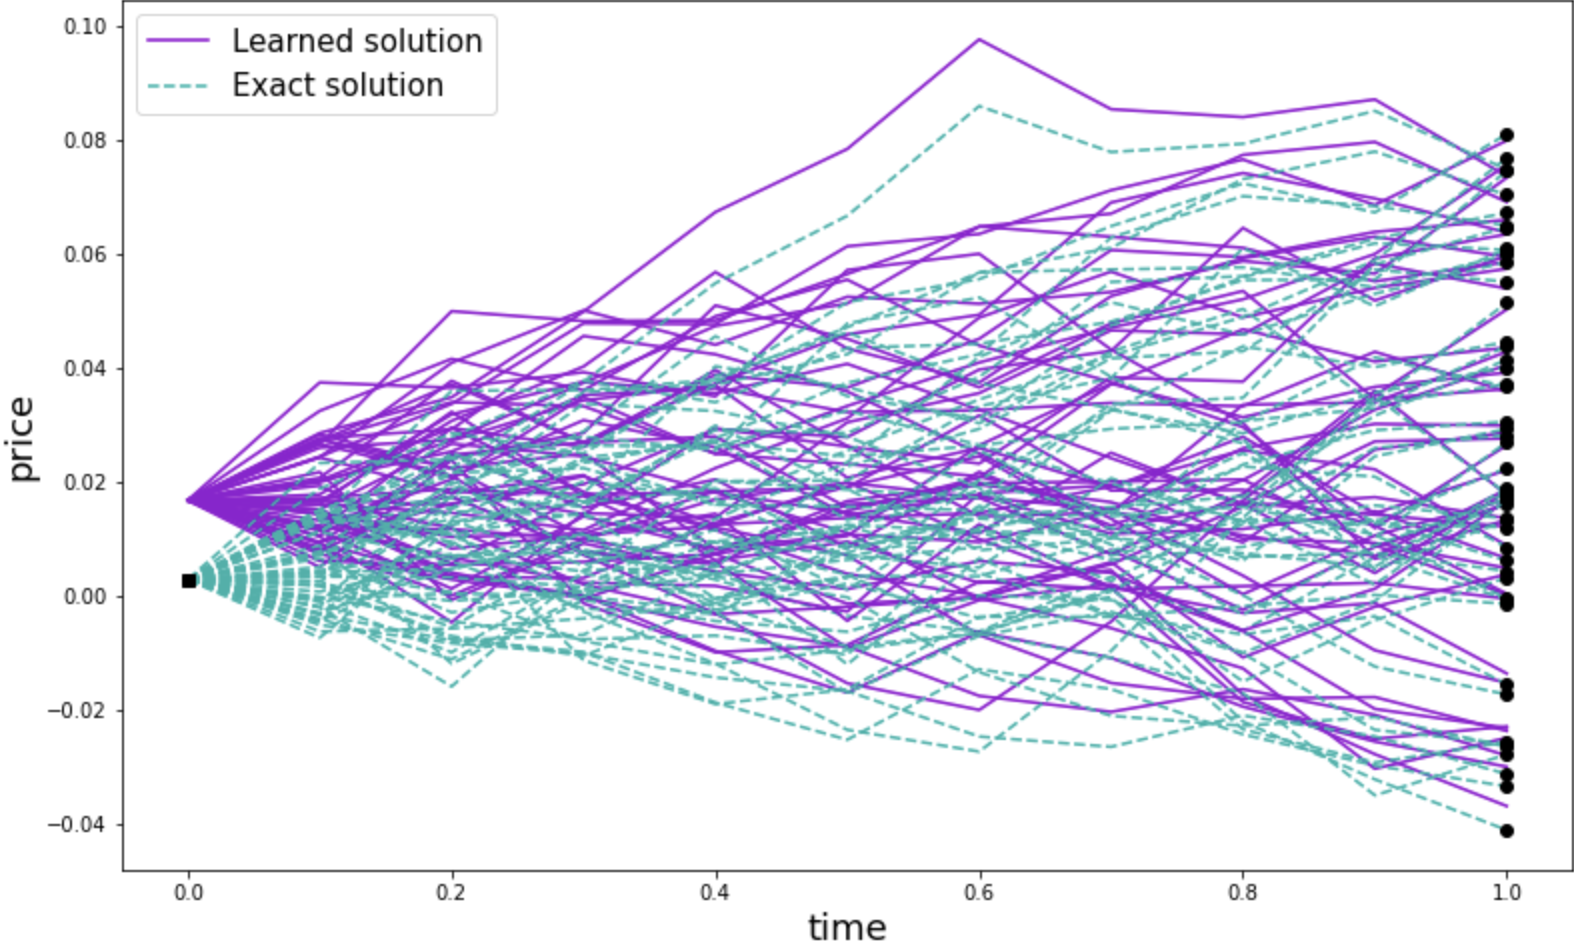
\includegraphics[scale=0.33]{irs.jpg}
		\caption{result of interest rate swap}
		\label{fig:zcp}
	\end{figure}
	Building upon the successful results obtained thus far, we proceed with the testing of the Bermudan swaption. To establish a benchmark for evaluation, we utilize the numerical solution provided by the \texttt{tf\_quant\_finance} library. We evaluate the initial price of the swaption at various states and parameters, comparing them to the benchmark to assess the level of closeness. For these experiments, we set the fixed rate at 0.02. Then we change the volatility and report the result again
	\begin{table}[htbp]
		\centering
		\begin{tabular}{cccc}
			\hline
			$\sigma$&$\theta_r = r_0$  & price from operator & benchmark \\
			\hline
			\multirow{5}{*}{0.03} &0.040 & 0.0487  & 0.0463 \\
			&0.045 & 0.0543  & 0.0529 \\
			&0.050 & 0.0561  & 0.0579 \\
			&0.055 & 0.0685  & 0.0672 \\
			&0.060 & 0.0761  & 0.0745 \\
			\hline  
			\multirow{5}{*}{0.05} & 0.040 & 0.0669  & 0.0602 \\
			&0.045 & 0.0693  & 0.0657 \\
			&0.050 & 0.0742  & 0.0714 \\
			&0.055 & 0.0819  & 0.0774 \\
			&0.060 & 0.0911  & 0.0835 \\
			\hline
			
		\end{tabular}
		\caption{Result of the Bermudan Swaption price comparison with $\kappa=0.4$ and $\sigma=[0.03, 0.05]$. The first colume give the level of the flatten forward rate curve at initial time; The second colume (price from operator) gives the price of Bermudan swaption calculated from the trained operator at initial time; The third colume is the same price given by the benchmark from \texttt{tf\_quant\_finance} library}
		\label{tab:structure1}
	\end{table}
	We observe that as the input parameter approaches the sample boundary, the magnitude of the error increases significantly. Furthermore, the operator demonstrates the capability to learn the relationship between price and volatility, exhibiting monotonic behavior. Another test to assess the Bermudanarity of the swaption involves substituting the analytical solution with the continuation value of the second sub-time interval. Since the continuation value of the final time interval corresponds to the European swaption, which possesses a closed-form solution, this approach effectively eliminates the error introduced by the terminal condition. Consequently, we can examine whether the resulting error is smaller than the benchmark or not. The price yield from the analytical continuation value is denoted as price (cont. from ana.) while the price from the last network inference is denoted as  price (cont. from net).
	\begin{table}[htbp]
		\centering
		\begin{tabular}{ccccc}
			\hline
			$\sigma$&$\theta_r = R_0$  & price (cont. from net) & price (cont. from ana.) &benchmark \\
			\hline
			\multirow{5}{*}{0.03} &0.040 & 0.0487 & 0.0477& 0.0463 \\
			&0.045 & 0.0543  & 0.0533 & 0.0529 \\
			&0.050 & 0.0561  & 0.0577 & 0.0579 \\
			&0.055 & 0.0685  & 0.0681  &0.0672 \\
			&0.060 & 0.0761  & 0.0751  &0.0745 \\
			\hline  
			\multirow{5}{*}{0.05} &0.040 & 0.0669  & 0.0613& 0.0602 \\
			&0.045 & 0.0693  & 0.0662 & 0.0657 \\
			&0.050 & 0.0742  & 0.0717 & 0.0714 \\
			&0.055 & 0.0819  & 0.0795 & 0.0774 \\
			&0.060 & 0.0911  & 0.0864 & 0.0835 \\
			\hline
			
		\end{tabular}
		\caption{The first colume give the level of the flatten forward rate curve at initial time; The second colume (price from operator) gives the price of Bermudan swaption calculated from the trained operator at initial time; The third colume gives the Bermudan swaption price when the continuation value is calculated by analytical solution rather then the neural operator trained from the last time interval; The fourth colume is the same price given by the benchmark from \texttt{tf\_quant\_finance} library}
		\label{tab:structure1}
	\end{table}
	We can find that the main issue of this algorithm is that training a single operator step by step may accumulate error. If the error of the last time step is not tiny enough, the continuation value given by the last step will not be accurate and therefore the final price would be far from the true value. However this issue happens in all numerical schemes and what we need to do is to polish our deep learning algorithm and train more steps with more suitable hyper parameters so that we can price long time period Bermudan products with more accuracy.
	\subsubsection{Bermudan Put Options}
	In this discussion, we examine the basket put option and Asian option under Heston model and evaluate them using the method proposed by Longstaff and Schwartz in \cite{longstaff2001valuing} (The algorithm is ahown in the appendix). While another benchmark in high dimensions is proposed by Lapeyre et al. in \cite{lapeyre2021neural}, we focus on lower-dimensional cases to test the convergence of our algorithm, without loss of generality. To generate sampling parameters that generate coefficients, we use the same setting as in the non-Bermudan cases, except for the strike, where we need more sampling in the OTM region. We sample the moneyness in $k \sim N(1.6, 0.3)$, given $K = S_0 \cdot k$, where $S_0 = S_0^1 = \cdots = S_0^d$. The payoff of European basket is given by:
	\begin{equation*}
		g(S_T; a) = \left\{K-\sum_{i=1}^d S_T^i, 0\right\}
	\end{equation*}
	The payoff of Asian is given by:
	\begin{equation*}
		g(S_T, A_T; a) = \left\{K-\sum_{i=1}^d A_T^i, 0\right\}
	\end{equation*}
	We calculate the absolute error (AE) of the initial prices compared to the prices given by Monte Carlo methods at different iterations. In contrast to European and path-dependent cases, we also track the value of $\frac{1}{B}\sum_{j=1}^Bvar(Y^{a_j}_0$), since this is an upper bound of the distance between the estimated control terms and their ground truth, as concluded in \cite{gao2022convergence}:
	\begin{equation*}
		\sup _{t \in[0, T]} \mathbb{E}\left|Y_t-Y_{\pi(t)}^\pi\right|^2+\int_0^T \mathbb{E}\left|Z_t-Z_{\pi(t)}^\pi\right|^2 \mathrm{~d} t \leq C\left[\Delta t+\operatorname{Var}\left(Y_0^\pi\right)\right]
	\end{equation*}
	Where $(Y_{\pi(t)}^\pi, Z_{\pi(t)}^\pi)$ is the approximated solution and $(Y_{t}, Z_{t})$ is the true solution. Then we show the result table under different dynamics:
	\begin{table}[H]
		\centering
		\begin{tabular}{cccccc}
			\hline$d$ & iteration & $\begin{array}{c}\text{MAE} \\
				\text{mean (std.)} \end{array}$   & mean of $var(Y_0)$  \\
			\hline \multirow{4}{*}{basket} & 100 & 0.9283 (0.3524) & 0.928 \\
			& 200 & 0.2572 (0.2012) & 0.067 \\
			& 500 & 0.1103 (0.0928) & 0.008 \\
			& 1000 & 0.0502 (0.0331) & 0.006 \\
			
			\hline \multirow{4}{*}{Asian} & 100 & 1.2725 (0.7673) & 1.104 \\
			& 200 & 0.3386 (0.258) & 0.082 \\
			& 500 & 0.0873 (0.0585) & 0.011 \\
			& 1000 & 0.0722 (0.0411) & 0.008 \\
			
			\hline
		\end{tabular}
		\caption{results of Bermudan products under Heston model}
		\label{tab:my_label}
	\end{table}
	\noindent We give the box plots for two experiments for comparing the initial prices from a batch input coefficients draw from the distribution:
	\begin{figure}[h!]
		\centering
		\subfigure[basket $d=3$]{\includegraphics[width = 0.4\textwidth]{box_plot2.png}}
		\quad
		\subfigure[Asian $d=3$]{\includegraphics[width = 0.4\textwidth]{box_plot1.png}}
		\caption{The left boxplot is the comparison between the predicted prices and true prices under a batch of input coefficients (functions) from time dependent GBM while the right one is from time dependent Heston model}
		\label{fig:path}
	\end{figure}
	Based on the results, it is evident that the initial variance converges. However, the comparison of prices reveals that the predicted value exhibits skewness as compared to the benchmark solution. This indicates that the method proposed by Wang in \cite{wang2018deep} has a certain degree of bias. Nonetheless, pricing Bermudan options using an operator may pose some potential issues worth discussing. Firstly, the most vital problem in Bermudan pricing is to recursively approximate the continuation value functions. However, extending it to operator learning would mean dealing with thousands times of sample paths than function approximation problems, making it challenging to efficiently approximate the operator. Secondly, the initial variance of the value iterated from the terminal value plays a crucial role in constructing the loss function in Bermudan problems and backward BSDE problems. Nevertheless, data in operator learning problems may not provide enough sample paths under each input coefficient, and increasing the batch size of coefficients and the number of paths for each coefficient may result in out-of-memory issues. Therefore, attaining a balance between the sample volume of coefficients and the volume of Monte Carlo paths is a significant challenge. Thirdly, for lower bias pricing, one possible approach is proposed by Liang in \cite{liang2021deep}, which combines least square with backward learning. However, in operator learning, extending this approach is challenging because an extra training task cannot be performed within the computational graph. Therefore, it remains a challenge to calculate the loss (construct graph) and perform least square at exercise dates simultaneously. One possible solution is to assume that continuous value operators in our problem have an analytical or quasi-linear form, similar to linear regression. This would allow us to perform least square without additional training while constructing the loss function of BSDEs. 
	\fi
	
	
	
	\section{Extensions}
	\subsection{Under Jump Processes}
	\subsubsection{Loss Function}
	We only discuss finite activity case. In this subsection we assume that the jumps are those of a compound Poisson process. Without loss of generality, we discuss the Merton diffusion model under time dependent GBM. We denote the intensity  as $\lambda$ for each asset and the levy measure for each asset is $\nu^i(\mathrm{d} z) = \lambda \varphi(z) \mathrm{d} z, i=1,\cdots,d$ with $\lambda > 0$ and $\varphi(z) = \frac{1}{\sqrt{2 \pi} \sigma_J}e^{{-\frac{1}{2}}\left( \frac{x - \mu_J}{\sigma_J}\right)^2} $ for each $z^i$ of each asset. Then the SDE of this process of the $i$-th underlying asset under risk neutral measure can be written as:
	\begin{equation*}
		\frac{\mathrm{d} S_t^i}{S_{t-}^i}=r(t) \mathrm{d} t+\sigma^i(t) \mathrm{d} W^{i}_t+\int_{\mathbb{R}}\left(e^{z^i}-1\right) \tilde{N}^i\left(\mathrm{d} z, \mathrm{d} t\right)
	\end{equation*}
	Then the related BSDE is:
	\begin{align*}
		-\mathrm{d}Y_t &= -r(t) Y_t \mathrm{d} t - (Z_t)^{\top}  \mathrm{d} W_t - \int_{\mathbb{R}}U(t,z) \tilde{N}\left(\mathrm{d} z, \mathrm{d} t\right) \\
		Y_T &= g(X_T; a)
	\end{align*}
	where $U(t, z) = u(t, S_{t-}e^z) - u(t, S_{t-})$. We now discuss the discretized scheme of both SDE and BSDE with jump diffusion. For  SDE, we have the solution, for any $i = 1, \cdots, d$:
	\begin{equation}\label{eq:jumpSDE}
		S_T^i=S_t^i \exp \left\{\left(\tilde{r}-\frac{\tilde{\sigma}^{2, i}}{2}\right)(T-t)+\tilde{\sigma}^i W_t^{i}-\int_{\mathbb{R}}\left(e^z-1-z\right) \nu^i(\mathrm{d} z)(T-t)+\int_t^T \int_{\mathbb{R}} z \tilde{N}^i(\mathrm{d} z, \mathrm{d} s)\right\}
	\end{equation}
	Then it is suffice to simulate the process of $ln(S_t)$. We have the following discretization scheme:
	\begin{align}\label{eq:discSDE}
		\ln S^m_{t_{n+1}} = \ln S^m_{t_{n}} + \left(r(t_n) \boldsymbol{1}-\frac{\sigma^2(t_n)}{2} - \lambda\left(e^{\mu_J + \frac{\sigma^2_J}{2}} - 1\right) \boldsymbol{1} \right)\Delta t +  \sigma(t_n)\circ\Delta W^m_{t_n} +\sum_{j=N_{t_n}}^{N_{t_{n+1}}}z_j
	\end{align}
	For the BSDE, we discretize it as 
	\begin{align}\label{eq:disc-jumpBSDE}
		Y_{t_N} & = g(X_{t_N}; a),  \\
		Y_{t_n} &\approx Y_{t_{n+1}} - r(t_{n+1}) Y_{t_{n+1}}\Delta t  -  Z_{t_n}^\top \Delta W_{t_n}-
		\sum_{j=N_{t_n}}^{N_{t_{n+1}}}\left(u(t_n, S_{t_n}e^{z_j}) - u(t_n, S_{t_n})\right) - \\
		&\Delta t \int_{\mathbb{R}^d}\left(u(t_n, S_{t_n}e^{z}) - u(t_n, S_{t_n})\right)\nu(\mathrm{d}z) , n=N-1,\cdots,0. 
	\end{align}
	For the discretization of BSDE,  we take care about the term: $\int_{\mathbb{R}}U(t,z) \tilde{N}\left(\mathrm{d} z, \mathrm{d} t\right) $. It can be decomposed as: $\sum_{j=N_{t_n}}^{N_{t_{n+1}}}\left(u(t_n, S_{t_n}e^{z_j}) - u(t_n, S_{t_n})\right) - \Delta t \int_{\mathbb{R}^d}\left(u(t_n, S_{t_n}e^{z}) - u(t_n, S_{t_n})\right)\nu(\mathrm{d}z)$. The question is of approximating the compensator term. The first option, which is feasible when the dimension $d$ is low, is to employ a standard quadrature rule. When the dimension increases on can resort to Monte Carlo integration. However, the training of the networks we introduced involves a further Monte Carlo simulations during the training phase, so that such approach would lead to costly nested Monte Carlo simulations. The alternative approach is proposed by \cite{gnoatto2022deep} where they approximate the compensator with another set of neural networks. Thus in this problem we approximate the term with an another unified operator network $w_{\rho}(t, x; a)$. Then we can put this constraint into the penalty function:
	\begin{equation*}
		\mathbb{E}\left[\left(\sum_{j=N_{t_n}}^{N_{t_{n+1}}}\left( u(t_n, S_{t_n}e^{z_j}) - u(t_n, S_{t_n})\ \right)-\Delta t w_{\rho}\left(t_n, S_{t_n}; a\right)\right)^2\right]
	\end{equation*}
	Then we give the loss function construction of the inner loss $\mathcal{L}(\theta,\rho; a)$ via following steps:
	\begin{itemize}
		\item  For $m=1,\cdots, M$, generate a path of the price process for each asset using Euler scheme. On each path, calculate the related states at each time point. We denote the state vector at time $t_n$ of asset $i$ on path $m$ by $X_{t_n}^{i,m}$ and $X_{t_n}^{m}$ is the collection of all $X_{t_n}^{i,m}$. We also keep the generated Brownian increment path $\{\Delta W_{t_n}^m: n=0,\cdots, N-1\}$ and jump increments.
		
		\item Step 2: For $n=0,...,N-1$ and $m=1,...,M$, calculate 
		\begin{equation}\label{eq:Z}
			Z_{t_n}^m = \sigma(t)\circ S_{t_{n}}\circ\nabla_X G_{\theta}(a, t_{n}, X_{t_n}^{m}),	
		\end{equation}
		This is the hedging ratio for the product during the time interval without early exercise.
		
		\item Step 3: Evaluate the BSDE value $Y_{t_n}^m$ with:
		\begin{align}
			Y_{t_N} & = g(X_{t_N}; a),  \\
			Y_{t_n} &\approx Y_{t_{n+1}} - r(t_{n+1}) Y_{t_{n+1}}\Delta t  -  Z_{t_n}^\top \Delta W_{t_n}-
			\sum_{j=N_{t_n}}^{N_{t_{n+1}}}\left(u(t_n, S_{t_n}e^{z_j}) - u(t_n, S_{t_n})\right) - \\
			&\Delta t w_{\rho}\left(t_n, S_{t_n}; a\right) , n=N-1,\cdots,0. 
		\end{align}
		
		\item Step 4:  The loss function of the model $\mathcal{L}_{model}(\theta, \rho; a)$ is given by the output from step 4 in the last subsubsection, i.e., 
		\begin{equation}\label{eq:loss-jump-a}
			\mathcal{L}_{m}(\theta, \rho; a)=\frac{1}{M}\sum_{m=1}^M\sum_{n=0}^N\left(G_{\theta}(\tilde{a}, t_{n}, X_{t_n}^m) - Y_{t_n}^m \right)^2.
		\end{equation}
		and the penalty function is given by:
		\begin{equation}\label{eq:penalty-jump-a}
			\mathcal{L}_{penalty}(\theta, \rho; a) =\frac{1}{N}\sum_{n=0}^{N-1} \left(\sum_{j=N_{t_n}}^{N_{t_{n+1}}}\left( u(t_n, S_{t_n}e^{z_j}) - u(t_n, S_{t_n})\ \right)-\Delta t w_{\rho}\left(t_n, S_{t_n}; a\right)\right)^2
		\end{equation}
		Then the loss function is:
		\begin{equation}
			\mathcal{L}(\theta, \rho; a)  = \mathcal{L}_{model}(\theta, \rho; a) + \mathcal{L}_{penalty}(\theta, \rho; a) 
		\end{equation}
	\end{itemize}
	To obtain $\mathcal{J}(\theta)$, we need to sample $a$ from distribution $\mu$. Suppose that we have a batch of sampled coefficients $\left\{a_1,\cdots,a_B\right\}$. We calculate $\mathcal{J}\left(\theta\right)$ by 
	\begin{equation}\label{eq:total-loss}
		\mathcal{J}\left(\theta,\rho\right) = \frac{1}{B}\sum_{j=1}^B \mathcal{L}(\theta, \rho; a_j).
	\end{equation}
	
	\noindent \textbf{Testing Design}: On method to test the loss function is to plug the analytical solution into the loss function to check whether the loss function value is close to zero. For BSDE under Merton jump diffusion model, the analytical solution can be written as a series form of BS formulas with different implied volatility values. We can expand this series to a certain order and check whether the loss function value is below a certain value. This series form solution as given as:
	\begin{align}
		V(S, K, T, r, \sigma, m, s, \lambda)=\sum_{k=0}^{\infty} \frac{e ^{-\bar{m} \lambda T}(\bar{m} \lambda T)^{k}}{k !} V_{B S}\left(S, K, T, r_{k}, \sigma_{k}\right)
	\end{align}
	where $\sigma_{k}=\sqrt{\sigma^{2}+k \frac{s^{2}}{T}}$ and $r_{k}=r-\lambda(\bar{m}-1)+\frac{k \ln (\bar{m})}{T}$ where $\bar{m} = e^{m + s^2/2}$. 

\subsubsection{Algorithm of European Style Products} \label{sec:euro_jump}
We summarize the training framework of European style problem on a certain time interval $[T_1, T_2]$. In this framework, the initial time $t_0$ is corresponded to $T_1$ and terminal time $T$ is corresponded to $T_2$. The algorithm is states as following procedure:

\begin{algorithm} [htbp!]
	%\caption{Training of the PONet}
	\begin{algorithmic}[htbp!] 
		\caption{Training of the Pricing Operator Network on $[T_1, T_2]$ under Jump Diffusions}\label{alg:euro_algo_jump}
		\STATE Specify the sampling distribution $\mu$ and initialize $\theta$.
		\FOR{$i= 1, 2,...$}{ 
			\STATE Sample a batch of coefficients  $\left\{a_j,\ j=1,\cdots, B\right\}$ from $\mu$.
			\STATE For each $j$, generate $M$ asset price paths on $[T_1, T_2]$ under $a_j$ and calculate $\mathcal{L}(\theta, \rho; a_j)$. .
			\STATE Calculate $\mathcal{J}(\theta, \rho)$. 
			\STATE Update $(\theta, \rho)$ by gradient descent. 
		}
		\ENDFOR
		\RETURN  RETURN The well trained operator network $u_{\theta}(t, x; a)$ defined on $[T_1, T_2]$.
	\end{algorithmic}
\end{algorithm}
\noindent Then for early exercise cases, things are same as previous discussion.

\subsubsection{Case 1: Callable Yield Note under Stochastic Volatility Jump Model}
\noindent \textbf{Stochastic Volatility Jump (SVJ)} There is strong evidence that stochastic volatility models cannot handle short-term smiles properly. The addition of jumps makes these models more realistic: Under the model first proposed by Bates \cite{bates1996jumps}, the jump term is the Merton jump diffusion and the distribution of jump size is under logrithm normal distribution. The dynamics can be described as:
\begin{align*}
	d S_t & =(r(t)-\lambda m) S_t d t+\sqrt{V_t} S_t d W^s_t + \left(e^J-1\right) S_t d N_t \\
	d V_t & =\kappa(\theta-V_t) d t+\varepsilon \sqrt{V_t} d W^v_t
\end{align*}
where $\kappa$ is a mean-reverting rate, $\theta$ is a long-term variance, $\epsilon$ is a volatility of volatility, $W^v_t$ and $W^s_t$) are correlated Wiener processes with constant correlation $\rho$. $\lambda$ is the intensity $J$ is the random variable representing the jump size with the law  $\nu(\cdot)$ and $m  = \mathbb{E}_{\nu}\left[\left(e^J-1\right)\right]$ which is the relative mean of jump size.

\noindent \textbf{BSDE}  By Ito lemma, the BSDE under SVJ is given as:
\begin{align*}
	-\mathrm{d}Y_t = -r(t) Y_t \mathrm{d} t - (Z_t)^{\top}  \mathrm{d}\boldsymbol{W}_t- \int_{\mathbb{R}}U(t,z) \tilde{N}\left(\mathrm{d} z, \mathrm{d} t\right) 
\end{align*}
where $\boldsymbol{W}_t = (W^s_t, W^v_t)$ and:
\begin{align*}
	\int_{\mathbb{R}}U(t,z) \tilde{N}\left(\mathrm{d} z, \mathrm{d} t\right)  =  \left(u(t_n, S_{t_n}e^J) - u(t_n, S_{t_n})\right) \mathrm{d} N_t- \Delta t \int_{\mathbb{R}^d}\left(u(t_n, S_{t_n}e^{z}) - u(t_n, S_{t_n})\right)\nu(\mathrm{d}z)
\end{align*}
Then since we have BSDE, we introduce the callable yield note.

\noindent \textbf{Callable Yield Note}: Callable Yield Notes allow investors to receive interest payments, regardless of the movements in the underlying. The CYNs will return the principal amount if the underlying does not reach or breach the Knock-In Level at the end of the trade (Some CYN is at any time during the trade). Otherwise, investors may receive less than 100\% of the principal amount relative to the percentage change of the underlying. Furthermore, the Issuer has the right to call the CYNs. If the CYNs are called, investors will receive 100\% of the principal amount plus any accrued but unpaid interest.
The upside of CYN is that it provides high yield if the notes are called prior to maturity on one of the specified call dates, or if held to maturity and the underlying has not breached the specified Knock-In Level. The downside is that If the notes are not called prior to maturity, the notes are not principal protected and if the Knock-In Level is breached, adverse performance of the underlying could result in a loss of principal. Then we try to formuarize the payment of the CYN. Denote the callable dates as $\mathcal{T}:=\left\{\tau_0=0, \tau_1, \ldots, \tau_k,\cdots,\tau_N=T\right\}$.  Denote the annualized coupon as $c$ and the barrier level of knock-in as $B$. Then from the perspective of the investor, the payoff of the trade is:
\begin{align}
	g(\tau_k, S_{\tau_k}; a) &= c \cdot (\tau_k - \tau_0), k=1,\cdots,N-1 \\
	g(\tau_N, S_{\tau_N}; a) &= c \cdot (\tau_N - \tau_0) - \max(B - p_T, 0)
\end{align}
where $p_t$ is the relative percentage of the initial value fot the basket of assets:
\begin{align*}
	p_t=\min _{j \in\{1,2, \cdots, d\}}\left[\frac{S^j_t}{S^j_0}\right]
\end{align*}
Then the dynamic programming rule is given as:
\begin{align}
	u(\tau_N, S_{\tau_N}; a) &= g(\tau_N, S_{\tau_N}; a)\\
	v(\tau_k, S_{\tau_k}; a) &= \mathbb{E}\left[e^{-\int_{\tau_k}^{\tau_{k+1}} r(s) ds}u\left(\tau_{k+1}, S_{\tau_{k+1}}; a\right) \mid S_{\tau_{k}} \right] , (k = 0,\cdots, N-1),\\
	u(\tau_k, S_{\tau_k}; a) &= \min \left\{g(\tau_k, S_{\tau_k}; a),  v(\tau_k, S_{\tau_k}; a)\right\}
\end{align}
Since the issuer is the early exercise side, the investor should use the minimum to do the dynamic programming. Finally, we can use the general algorithm to price this CYN.
Then the product can be priced and hedged with the algorithm \ref{sec:algo2}.
The clarified issue is:
\begin{enumerate}
	\item Coefficients: $a = (r(t), \kappa, \theta, \epsilon, \lambda, m, s, \rho, c, B,  K)$. (For callable Asian $a = (r(t), \kappa, \theta, \epsilon, \lambda, m, s, \rho,  K)$)
	\item The terminal payoff is 	$g(\tau_N, S_{\tau_N}; a) = h(\tau_N, S_{\tau_N}) = c \cdot (\tau_N - \tau_0) - \max(B - p_T, 0)$. (For callable Asian the payoff is $\left(\frac{1}{d}\sum_{i=1}^dA^i_T - K \right)^{+}$)
	\item The early exercise payoff is: $g(\tau_k, S_{\tau_k}; a) = h(\tau_k, S_{\tau_k}) = c \cdot (\tau_k - \tau_0), k=1,\cdots,N-1 $. (For callable Asian the payoff is $\left(\frac{1}{d}\sum_{i=1}^dA^i_t - K \right)^{+}$)
	\item no Markovian Variable. (For callable Asian, the variable is $A_t$ which is defined before)
\end{enumerate}

\noindent \textbf{Test Design}
In this product, we introduce two classes \texttt{StochaticVolJump} and \texttt{CallableYieldNote}. For \texttt{StochaticVolJump}, we intend to give following test method:
\begin{itemize}
	\item  \texttt{test\_drift}: This is to test the correctness of the drift function, we test the consistence of output shape and value of the function and the ground truth.
	\item  \texttt{test\_diffusion}: This is to test the correctness of the diffusion function, we test the consistence of output shape and value of the function and the ground truth.
	
	\item  \texttt{test\_jumpdiffusion}: This is to test the correctness of the jump diffusion function, we test the consistence of output shape and value of the function and the ground truth.
	
	\item (Reduce test) This test is just let the jump intensity $\lambda = 0$ and test whether all the test related to stochastic volatility without jump can pass.
	
	\item  \texttt{test\_martingale}: This is to test the martingale property for the SDE under risk-neutral measure via Monte Carlo simulation.
\end{itemize}

For \texttt{CallableYieldNote}, we intend to give following test method:
\begin{itemize}
	\item  \texttt{test\_payoff} This function is to test the payoff at each certain time point. We just need to test the shape and the output value
	
	\item \texttt{test\_martingale} We set the coupon become zero and the product reduced to the European put option. Then we test the MC price under this constraint and check whether this is closed to the Black-Scholes solution (In this test we just use the GBM as the SDE).
\end{itemize}


\subsubsection{Case 2: Stochastic Local Volatility Jump Model under Hull White Interest Rate}
Based on Heston Model, Merton jump diffusion model, Hull and White model and we combine all these issue togather and also introduce the local volatility surface $v(S, t)$ which fits the market prices and dividend payment $k(t)$. For simplicity, we use one factor Hull and White model to model the stochastic interest rate.  Then the final version of the most complicated model is demonstrated as follows:
\begin{align*}
	d R_t & = \kappa_r(\theta_r-R_t) d t+\varepsilon_r  d W^r_t\\
	d S_t/S_t & =(R_t - k(t) -\lambda m) d t + v(S_t, t)\sqrt{V_t}  d W^s_t + \left(e^J-1\right)  d N_t \\
	d V_t & =\kappa(\theta-V_t) d t+\varepsilon \sqrt{V_t} d W^v_t
\end{align*}
And as in previous discussion, we assume $J \sim \mathcal{N}(\mu_J, \sigma_J^2)$. And $d W^r_t dW^s_t = 0$, $d W^r_t dW^v_t = 0$, $d W^v_t dW^s_t = \rho^{s,v} dt$. Then, we can find that The BSDE can be represented as:
\begin{align*}
	-\mathrm{d}Y_t = -R_t Y_t \mathrm{d} t - (Z_t)^{\top}  \mathrm{d}\boldsymbol{W}_t- \int_{\mathbb{R}}U(t,z) \tilde{N}\left(\mathrm{d} z, \mathrm{d} t\right) 
\end{align*}
$Z_t$ is a function of $(R_t, S_t, V_t)$, $\boldsymbol{W}_t = (W^r_t, W^s_t, W^v_t)^{\top}$ . And
\begin{align*}
	\int_{\mathbb{R}}U(t,z) \tilde{N}\left(\mathrm{d} z, \mathrm{d} t\right)  &=  \left(u(t_n, R_{t_n}, S_{t_n}e^J, V_{t_n}) - u(t_n, R_{t_n}, S_{t_n}, V_{t_n})\right) \mathrm{d} N_t \\
	&- \left( \int_{\mathbb{R}^d}\left(u(t_n, R_{t_n}, S_{t_n}e^{z},  V_{t_n}) - u(t_n,R_{t_n},  S_{t_n}, V_{t_n})\right)\nu(\mathrm{d}z)\right) \mathrm{d}t
\end{align*}
In these BSDE solving problem. The coefficients are $a = (\kappa_r, \varepsilon_r, \theta_r, \lambda, m, \kappa, \theta, \varepsilon; k(t), v(s, t); \rho^{s,v})$
Then, again, we face with the callable yield note, the dynamic programming rule is given as:
\begin{align}
	u(\tau_N, R_{\tau_N}, S_{\tau_N}, V_{\tau_N}; a) &= g(\tau_N, S_{\tau_N}; a)\\
	v(\tau_k, R_{\tau_k}, S_{\tau_k}, V_{\tau_k}; a) &= \mathbb{E}\left[e^{-\int_{\tau_k}^{\tau_{k+1}} R_s ds} u\left(\tau_{k+1}, R_{\tau_{k+1}}, S_{\tau_{k+1}}, V_{\tau_{k+1}}; a\right) \mid R_{\tau_k}, S_{\tau_k}, V_{\tau_k} \right] , (k = 0,\cdots, N-1),\\
	u(\tau_k, R_{\tau_k}, S_{\tau_k}, V_{\tau_k}; a) &= \min \left\{g(\tau_k,  S_{\tau_k}; a),  v(\tau_k, R_{\tau_k}, S_{\tau_k}, V_{\tau_k})\right\}
\end{align}
The clarified issue is:
\begin{enumerate}
	\item Coefficients: $a = (\kappa_r, \varepsilon_r, \theta_r, \lambda, m, \kappa, \theta, \varepsilon; k(t), v(s, t); \rho^{s,v}, c, B,  K)$. (For callable Asian $a = (\kappa_r, \varepsilon_r, \theta_r, \lambda, m, \kappa, \theta, \varepsilon; k(t), v(s, t); \rho^{s,v},  K)$)
	\item The terminal payoff is 	$g(\tau_N, S_{\tau_N}; a) = c \cdot (\tau_N - \tau_0) - \max(B - p_T, 0)$. (For callable Asian the payoff is $\left(\frac{1}{d}\sum_{i=1}^dA^i_T - K \right)^{+}$)
	\item The early exercise payoff is: $g(\tau_k, S_{\tau_k}; a) = c \cdot (\tau_k - \tau_0), k=1,\cdots,N-1 $. (For callable Asian the payoff is $\left(\frac{1}{d}\sum_{i=1}^dA^i_t - K \right)^{+}$)
	\item no Markovian Variable. (For callable Asian, the variable is $A_t$ which is defined before)
\end{enumerate}
\noindent \textbf{Test Design}
We introduce the class \texttt{StochaticLocalVolJump}. We test this class with the same rule as testing previous classes related to SDEs. Since the drift and diffusions are almost same as previous ones. We just test the Euler step method to check whether the value at the next time step has the potential distribution.
\begin{itemize}
	\item \texttt{test\_conditional\_distribution}: Do a one step forward simulation with sufficient large number of paths. We test whether the mean and the variance is consistence with the drift and diffusions.
	\item \texttt{test\_cholesky}: Sample a vector and calculate the quadatic form corresponded to the decomposed matrix to check whether it is non negative. 
	\item  \texttt{test\_martingale}: This is to test the martingale property for the SDE under risk-neutral measure via Monte Carlo simulation.
\end{itemize}

\subsection{Experiments}
To be completed...

	
	
	
	
	\section{Conclusions}\label{sec:conclusion}
	\noindent \textbf{1. Conclusions} In the study of derivatives pricing with operator network, we have developed a neural network model to learn the mapping from the space of time, states, and coefficients to the derivative price. Our method is based on the representation of the pricing function by basis expansion, which separates the effect of coefficients on the price from that of time and states. We use separate neural networks called branch and trunk nets to capture these effects. We also introduce the embedding net to generate latent representations of the coefficient functions and the PI net to produce the theoretical property of permutation invariance that holds in many multi-asset derivatives. To train the neural network model, we construct a loss function by solving the BSDE associated with the pricing problem. The BSDE approach is flexible as it provides a unified framework to price different types of derivatives in general price models. Various numerical experiments demonstrate the ability of our model in learning this complicated mapping even in the multi-dimensional case. In future research, we plan to extend the current method to consider options with early exercise features and price models with jumps.
	
	
	\noindent \textbf{2. Problems} In Bermudan pricing, the key challenge is to approximate the continuation value functions recursively. This process involves solving a sequence of conditional expectation problems, which can be computationally expensive. However, if we can solve this problem effectively, the Bermudan problem can be reduced to a European and path-dependent problem. This is because the Bermudan option can be viewed as a series of European options with the possibility of early exercise at specific dates. Furthermore, since the option's payoff depends on the underlying asset's price path, it is also a path-dependent option. Therefore, if we can accurately approximate the continuation value operators, we can effectively reduce the Bermudan problem to a combination of European and path-dependent options. This can significantly simplify the pricing process and make it more computationally efficient. However, as mentioned earlier, the challenge lies in efficiently approximating the continuation value operators, which is a non-trivial task.
	
	\noindent \textbf{3. Extensions}
	To prepare for future extensions, one interesting topic is operator training under jump models. The Merton diffusion model and SVJ (stochastic volatolity jump) model are the counterparts of GBM and Heston models, respectively. Fortunately, \cite{gnoatto2023deep} has proposed a framework for Deep BSDE under jump models. The innovation lies in their use of an extra neural network to approximate the expectation of the jump term in high-dimensional cases, which allows for the extension of all deep BSDE without jump using this technique. When it comes to Bermudan pricing, we realize that the approximation of continuation value functions (operators) is independent of the formulation of the underlying asset dynamics or stochastic volatility. Thus, all we need to do is perform least squares with paths generated by Monte Carlo simulation. Once we have the value network, we can use dynamic programming to obtain the intrinsic value on each exercise date under each scenario. We can then use the framework of \cite{gnoatto2023deep} once again to train the pricing operator with PricingONet proposed by our paper. In other words, whether under a jump model or not, the core problem is to design a framework to efficiently train the operator mapping from coefficients to continuation value functions\ref{appendix}. Finally, experiments with jump need to be tested in future research given all kinds of products without jump pass test.
	
	
	
	
	
	\appendix \label{appendix}
	\section{Some Analytical Solutions}
	Here we list benchmark solutions under time dependent GBM.
	\iffalse
	\section{Least-Squares Monte Carlo}
	he least-squares Monte Carlo (LSMC) method, proposed by \cite{longstaff2001valuing}, is a method of early-exercisable option pricing in which regression calculation uses simulation sample paths. In the LSMC method, a polynomial function of the Markov process state variables is applied to identify the continuation values. The following is an algorithm for Bermudan option pricing using the LSMC method.
	\begin{itemize}
		\item Step 0: Generate Monte Carlo sample paths of the underlying asset prices and state vari-
		ables. We denote the underlying asset prices at time $t$ in the $j$-th sample path as $S^{(j)}_t$ and the Markov process state variables as $x^{(j)}_t$. Subsequently, we obtain the series of paths as:
		\begin{equation*}
			\begin{array}{cccccccc}
				S_{T_1}^{(1)}, & S_{T_2}^{(1)}, & \ldots, & S_{T_N}^{(1)} & x_{T_1}^{(1)}, & x_{T_2}^{(1)}, & \ldots, & x_{T_N}^{(1)} \\
				S_{T_1}^{(2)}, & S_{T_2}^{(2)}, & \ldots, & S_{T_N}^{(2)} & x_{T_1}^{(2)}, & x_{T_2}^{(2)}, & \ldots, & x_{T_N}^{(2)} \\
				\vdots & \vdots & \vdots & \vdots & \vdots & \vdots & \vdots & \vdots \\
				S_{T_1}^{(M)}, & S_{T_2}^{(M)}, & \ldots, & S_{T_N}^{(M)} & x_{T_1}^{(M)}, & x_{T_2}^{(M)}, & \ldots, & x_{T_N}^{(M)}
			\end{array}
		\end{equation*}
		
		\item Step 1: Calculate the series of Bermudan option values at maturity $T_N = T$ as:
		\begin{equation*}
			V_{T_N}:=\left[g\left(S_{T_N}^{(1)}, x_{T_N}^{(1)}\right), g\left(S_{T_N}^{(2)},  x_{T_N}^{(2)}\right), \ldots, g\left(S_{T_N}^{(M)},  x_{T_N}^{(M)}\right)\right]^{\top}
		\end{equation*}
		where $g$ denotes a payoff function of $S_t$
		
		\item Step 2: Find a polynomial function that approximates the continuation values. Herein, we denote a polynomial function as $\hat{h}_{T_{N−1}}$ and a measurable function representing conditional expectation as $h_{T_{N-1}}$.  Then,
		\begin{equation*}
			h_{T_{N-1}}\left(S_{T_{N-1}}, x_{T_{N-1}}\right) \approx \hat{h}_{T_{N-1}}\left(S_{T_{N-1}}, x_{T_{N-1}}\right)
		\end{equation*}
		Additionally, $\hat{h}_{T_{N−1}}$ is sought to minimize the following least square objective:
		\begin{equation*}
			\frac{1}{M} \sum_{i=1}^M\left(\hat{h}_{T_{N-1}}\left(S_{T_{N-1}}, x_{T_{N-1}}\right)-e^{-r \delta_{T_N}} V_{T_N}\right)^2
		\end{equation*}
		
		\item Step 3: Calculate the approximated continuation values. Set set the
		series of approximated continuation values at $T_{N−1}$ as:
		\begin{equation*}
			\left[\hat{h}_{T_{N-1}}\left(S_{T_{N-1}}^{(1)}, x_{T_{N-1}}^{(1)}\right), \hat{h}_{T_{N-1}}\left(S_{T_{N-1}}^{(2)}, x_{T_{N-1}}^{(2)}\right), \ldots, \ldots, \hat{h}_{T_{N-1}}\left(S_{T_{N-1}}^{(M)}, x_{T_{N-1}}^{(M)}\right)\right]
		\end{equation*}
		
		\item Step 4: Calculate the exercised values and Bermudan option values.
		\begin{equation*}
			V_{T_{N-1}}\left(S_{T_{N-1}}^{(j)}, x_{T_{N-1}}^{(j)}\right):=\max \left(g\left(S_{T_{N-1}}^{(j)}, x_{T_{N-1}}^{(j)}\right), h_{T_{N-1}}\left(S_{T_{N-1}}^{(j)}, x_{T_{N-1}}^{(j)}\right)\right), j=1, \ldots, M
		\end{equation*}
		This makes target labels for next iteration.
		
		\item Step 5:Repeat Step 2 to Step 4 for possible exercise times until time $T_0$ A series of Bermudan option values for $V_{T_0}$ at time $T_0$ are obtained by repeating Step 2 to Step 4 backward to time $T_0$.
		
		\item Calculate the Bermudan option price $V_{T_0}$:
		\begin{equation*}
			\overline{V_{T_0}}=\frac{1}{M} \sum_{j=1}^M V_{T_0}^{(j)}
		\end{equation*}
	\end{itemize}
	Using this approach, we calculated the Bermudan option price using the continuation values from the polynomial function at each exercisable time. The main point of the pricing procedure in the LSMC method is that the polynomial function is defined to approximate the continuation values at each exercisable time point
	
	
	\begin{align} 
		& d_{+}=\frac{\ln \frac{F}{K}+\frac{1}{2} \tilde{\sigma}^2 \tau}{\tilde{\sigma} \sqrt{\tau}} \\ 
		& d_{-}=d_{+}-\tilde{\sigma} \sqrt{\tau}. \\
		&\sigma^2 =\frac{1}{n} \sum_{i=1}^n \sigma_i^2 \\ 
		&\tilde{\sigma}^2 =\frac{1}{n^2} \sum_{i, j=0}^n \rho_{i j} \sigma_i \sigma_j \\ 
		&F =\left(\prod_{i=1}^n S^i_0\right)^{\frac{1}{n}} \cdot \exp \left(-\frac{1}{2}\left(\sigma^2-\tilde{\sigma}^2\right) \tau\right)            
	\end{align}	
	
	\begin{align}
		&\sigma^2 =\frac{1}{n} \sum_{i=1}^n \frac{1}{T-t}\int_t^T\sigma_i^2(s) ds , \\ 
		&\tilde{\sigma}^2 =\frac{1}{n^2} \sum_{i, j=0}^n \rho_{i j} \frac{1}{T-t}\int_t^T\sigma_i(s)\sigma_j(s) ds  , \\
	\end{align}
	
	
	\fi
	
	
	\section{Analytical Solutions under Time-dependent GBM Cases} \label{appendix}
	We first show the analytical solution of vanilla European call option under time-dependent GBM, where we denote $N(\cdot)$ as the cumulative distribution function of standard normal distribution.
	\noindent \textbf{1-dimensional Black Scholes formula}: The closed form solution of European call option is:
	\begin{equation*}
		u\left(t, S_t; (r, \sigma, \kappa)\right)=S_t N\left( d_1\right) -  \kappa S_0 e^{-\tilde{r}(T - t)}N\left( d_2\right),
	\end{equation*}
	where 
	\begin{equation*}
		d_1 = \frac{\log\left(\frac{S_t}{ \kappa S_0}\right)+\left(\tilde{r} + \frac{\tilde{\sigma}^2}{2}\right)(T-t)}{\tilde{\sigma}\sqrt{T-t}}, \quad d_2 = d_1 - \sigma\sqrt{T-t}.
	\end{equation*}
	The spot rate and volatility terms under time dependent GBM is given as:
	\begin{align}
		& \tilde{r} = \frac{1}{T-t}\int_t^T r(s) ds   , \quad \tilde{\sigma}^2 = \frac{1}{T-t}\int_t^T\sigma^2(s) ds.
	\end{align}
	\noindent \textbf{1-dimensional float lookback option}: Follow the expression of the $\tilde{r}$ and $\tilde{\sigma}^2$, we give the formula of float strike minimum look back option and geometric Asian call option.
	\begin{equation*}
		u(t, S_t, m_t; (r, \sigma))=S_t N\left(a_1\right)-m_t e^{-\tilde{r}(T-t)} N\left(a_2\right)-S_t \frac{\tilde{\sigma}^2}{2 \tilde{r}}\left(N\left(-a_1\right)-e^{-\tilde{r}(T-t)}\left(\frac{m_t}{S_t}\right)^{2 \tilde{r} / \tilde{\sigma}^2} N\left(-a_3\right)\right).
	\end{equation*}
	where
	\begin{equation*}
		a_1=\frac{\log \left(S_t / m_t\right)+\left(\tilde{r}+\tilde{\sigma}^2 / 2\right)(T-t)}{\tilde{\sigma} \sqrt{T-t}}, \quad a_2=a_1-\tilde{\sigma} \sqrt{T-t}, \quad a_3=a_1-\frac{2 \tilde{r}}{\tilde{\sigma}} \sqrt{T-t}.
	\end{equation*}
	\noindent \textbf{1-dimensional geometric Asian call option formula}: The corresponded time dependent Asian formula under time dependent GBM is give as:
	\begin{equation*}
		u\left(t, S_t, A_t; (r, \sigma, \kappa)\right)=e^{-\tilde{r}(T-t)}\left(A_t^{t / T} S_t^{1-t / T} e^{\hat{\mu}+\hat{\sigma}^2 / 2} N\left(d_1\right)-\kappa S_0 N\left(d_2\right)\right),
	\end{equation*}
	where
	\begin{align}
		A_t & =\exp \left\{\frac{1}{t} \int_0^t \log S_s d s\right\}  , \quad \hat{\mu}  =\left(\tilde{r}-\frac{\tilde{\sigma}^2}{2}\right) \frac{1}{2 T}(T-t)^2  , \quad \hat{\sigma}=\frac{\tilde{\sigma}}{T} \sqrt{\frac{1}{3}(T-t)^3}, \\
		d_2 & =\frac{(t / T) \log A_t+(1-t / T) \log S_t+\hat{\mu}-\log K}{\tilde{\sigma}}  , \quad d_1 =d_2+\hat{\sigma} .
	\end{align}
	
	
	
	\noindent \textbf{Multi-dimensional geometric basket call option formula}: Then we show the analytical solution of geometric basket call:
	\begin{equation*}
		u\left(t, S_t ; (r, \sigma, \rho_S, \kappa)\right)=F N\left(d_1\right) - \kappa \bar{S_0} e^{-\tilde{r} (T-t)}N\left(d_2\right).
	\end{equation*}
	where $\bar{S_0} = \left( \prod_{i=1}^d S^i_0\right)^{\frac{1}{d}}$ denotes the geometric average of the initial price. 
	\begin{align} 
		d_{+} &=\frac{\ln \frac{F}{\kappa \bar{S_0}}+\frac{1}{2} \tilde{\sigma}^2 (T-t)}{\tilde{\sigma} \sqrt{(T-t)}} , \quad d_{-}=d_{+}-\tilde{\sigma} \sqrt{(T-t)}, F =\bar{S_0} \left(\left(\tilde{r}-\frac{\left(\sigma^2-\tilde{\sigma}^2\right)}{2}\right) (T-t)\right)  \\
		\sigma^2 &=\frac{1}{n} \sum_{i=1}^n \frac{1}{T-t}\int_t^T\sigma_i^2(s) ds , \quad \tilde{\sigma}^2 =\frac{1}{n^2} \sum_{i, j=0}^n \rho_{i j} \frac{1}{T-t}\int_t^T\sigma_i(s)\sigma_j(s) ds       
	\end{align}	
	under time dependent GBM, the spot rate $\tilde{r}$ is same as what in one dimensional cases
	
	
	
	
	\bibliographystyle{chicagoa}
	\bibliography{reference}
	
	
	
\end{document}














